%---------------------导言区---------------------------%
\documentclass[10pt,a4paper,twoside,UTF8]{ctexart}
\usepackage{geometry}%用于设置上下左右页边距
	\geometry{left=2cm,right=2cm,top=2.5cm,bottom=3cm}
\usepackage{xeCJK,amsmath,paralist,enumerate,booktabs,multirow,graphicx,subfig,setspace,listings}
	\setlength{\parindent}{2em}%正文首行缩进两个汉字
	\lstset{language=tex}
\usepackage{titlesec}
	\newfontfamily\sectionef{Times New Roman}
	\setCJKfamilyfont{FZHeiTi}{黑体}
	\newcommand{\sectioncf}{\CJKfamily{FZHeiTi}}
	\titleformat*{\section}{\large\bfseries\sectioncf\sectionef}
	\titleformat*{\subsection}{\normalsize\bfseries\sectioncf\sectionef}
\usepackage{fancyhdr}
\usepackage{float}
\usepackage{layout}
\setlength{\skip\footins}{0.5cm}%脚注与正文的距离
\renewcommand{\footnotesize}{}%设置脚注字体大小
\setlength\columnsep{0.8cm}%设置双栏的间距
\usepackage{ifthen}%这个宏包提供逻辑判断命令
\newboolean{first}%引入布尔变量
\setboolean{first}{true}%将布尔变量设置为true
\pagestyle{fancy}
	\fancypagestyle{maincontent}{
		\fancyhf{}  %清空页眉页脚设置
		\fancyhead[EL, OR]{\thepage}
		\fancyhead[EC]{实验C7 基于空间光调制器的光学实验}
		\fancyhead[OC]{基\quad 础\quad 物\quad 理\quad 实\quad 验}
		\renewcommand\headrulewidth{0pt}
	}

	\usepackage{datetime}
	\fancypagestyle{firstpage}{
		\setboolean{first}{false}%firstpage出现,则将first重置为false
		\fancyhf{}  %清空页眉页脚设置
		\fancyhead[L]{\the\year 年\the\month 月}
		\fancyhead[R]{\shortmonthname[\the\month], \the\year}
		\fancyhead[C]{
		\large{基\quad 础\quad 物\quad 理\quad 实\quad 验}\\
		\normalsize{GENERAL PHYSICS LABORATORY}
		}
	}

	%%% Step3 页眉线的设置:用布尔变量区分首页和正文
	\newcommand{\makefirstpageheadrule}{%定义首页页眉线-双线绘制命令
	\makebox[0pt][s]{\rule[0.6\baselineskip]{\headwidth}{0.3pt}}
	\makebox[0pt][s]{\protect\hspace{-0.34em}\rule[0.75\baselineskip]{\headwidth}{0.3pt}}
	\protect\vspace{-20pt}
	}

	\newcommand{\makeheadrule}{%定义正文页页眉线绘制命令,单线
	\makebox[0pt][l]{\rule[1\baselineskip]{\headwidth}{0.3pt}}
	\protect\vspace{-20pt}%页眉和正文的距离
	}

	%根据布尔变量first为true或false分别执行不同的页眉线绘制命令
	\renewcommand{\headrule}{%重定义headrule命令
	\ifthenelse{\boolean{first}}{\makeheadrule}
	{\makefirstpageheadrule}
	}
%%end--------------设置首页和正文不同的页眉页脚-----------%%



%%begin-----------------参考文献-----------------------%%
% \usepackage{cite}
% \newcommand{\upcite}[1]{\textsuperscript{\textsuperscript{\cite{#1}}}} %参考文献上标
%\usepackage[backref]{hyperref}

\usepackage{url}
\usepackage[colorlinks,linkcolor=blue,urlcolor=blue]{hyperref}%超链接
\usepackage[hyperref=true,backend=biber,bibstyle=gb7714-2015,citestyle=numeric-comp,sorting=none,backref=true]{biblatex}
	%hyperref=true和backref=true表示为各个参考文献的引用处、及定理、定义、例子等的引用处都添加上超链接;
	%backend=biber:后端处理的程序为biber.exe
	%bibstyle:参考文献风格;每个期刊、组织要求不同
		%gb7714-2015是目前国内期刊通用的风格,称为gb标准风格
	%citestyle:引用风格;每个期刊、组织要求不同
	%sorting=none:按照参考文献在论文中出现的先后顺序排序。
	%**编译:biblatex与biber命令配合使用。xelatex-biber-xelatex-xelatex
\addbibresource{ref.bib}
	%这里写上.bib文件的相对地址
	%每次实验引用的页数不同,需要手动改变

%%end-------------------参考文献-----------------------%%

%%——————————————————————代码框设置——————————————————————%%
\usepackage{listings}
\usepackage{color}

\definecolor{dkgreen}{rgb}{0,0.6,0}
\definecolor{gray}{rgb}{0.5,0.5,0.5}
\definecolor{mauve}{rgb}{0.58,0,0.82}

\lstset{ %
  language=Python,                % the language of the code
  basicstyle=\footnotesize,       % the size of the fonts that are used for the code
  numbers=left,                   % where to put the line-numbers
  numberstyle=\tiny\color{gray},  % the style that is used for the line-numbers
  stepnumber=1,                   % the step between two line-numbers. If it's 1, each line 
                                  % will be numbered
  numbersep=5pt,                  % how far the line-numbers are from the code
  backgroundcolor=\color{white},      % choose the background color. You must add \usepackage{color}
  showspaces=false,               % show spaces adding particular underscores
  showstringspaces=false,         % underline spaces within strings
  showtabs=false,                 % show tabs within strings adding particular underscores
  frame=single,                   % adds a frame around the code
  rulecolor=\color{black},        % if not set, the frame-color may be changed on line-breaks within not-black text (e.g. commens (green here))
  tabsize=2,                      % sets default tabsize to 2 spaces
  captionpos=b,                   % sets the caption-position to bottom
  breaklines=true,                % sets automatic line breaking
  breakatwhitespace=false,        % sets if automatic breaks should only happen at whitespace
  title=\lstname,                    % show the filename of files included with \lstinputlisting;
                                  % also try caption instead of title
  keywordstyle=\color{blue},          % keyword style
  commentstyle=\color{dkgreen},       % comment style
  stringstyle=\color{mauve},         % string literal style
  escapeinside={\%*}{*)},            % if you want to add LaTeX within your code
  morekeywords={*,...}               % if you want to add more keywords to the set
}
%%——————————————————————代码框设置——————————————————————%%
%%%%%%%%%%%%%%%%%%%%%%%%%%%%%%%%%%%%%%%%%%%%%%%%%%%%%%%%%%
%%%%%%%%%%%%%%%%%%%%%%%%%正文开始%%%%%%%%%%%%%%%%%%%%%%%%%%
%%%%%%%%%%%%%%%%%%%%%%%%%%%%%%%%%%%%%%%%%%%%%%%%%%%%%%%%%%

\begin{document}


%%begin-------------------中文摘要-----------------------%%
\title{\LARGE\textbf{实验C7 基于空间光调制器的光学实验}\footnotemark[1]}
\author{\large\textit{XXX\footnotemark[2]}
\\ \normalsize{(1. \textit{中山大学 物理学院,广东 广州 }510275)}}
\date{}%不显示日期


	%twocolumn: 双栏article下的单栏摘要
	\maketitle  %标题和作者
  	\renewcommand{\abstractname} {} %不显示摘要名字
	\begin{abstract}
	\vspace{-3em}
	% vspace:调整垂直空白,可以自己调整;缩小abstract和center(以及maketitle)的间距
	%\noindent %备用:摘要无缩进
	{\bf 摘{} 要:}
	{\small 
	本次实验通过使用空间光调制器(SLM),测量其振幅调制特性,测量基于SLM产生的光学畸变。
	利用多种光学仪器完成空间滤波、高通滤波、低通滤波、方向滤波以及完成数字全息与计算全息的实验。
	基于此了解傅立叶光学的基本内容。
	首先测量空间光调制器的振幅调制曲线,发现曲线整体呈 S 型,证明在偏振片正交的情况下,SLM 的透射率随写入信号的变化存
	在阈值电压和饱和电压。其次使用CCD 拍摄不同焦距的透镜,不同缩小倍数棋盘格畸变的情况,棋盘格成像均发生枕形畸变。发现成像中距离中心位置越
	近的点畸变越小,距离中心位置越远的点畸变越大。
	在空间频谱和滤波实验中,首先用两种不同的光路验证阿贝原理,然后分别用低通滤波、高通滤波、方向滤波过滤光波。
	通过低通滤波的像最终图像是消去了网纹的光字,而通过高通滤波器的像与原像相比,区别在于前者更容易观察细节,锐化度更高。
	这是因为高频代表的细节被保留,低频对应的像被削弱,相同的低频成分被滤去,所以提高了对比度。
    方向滤波狭缝的放置方式不同,导致部分信息丢失,只保留特定方向上的频率信息,所以最终成像也只有该方向上的振幅得以还原。
	最后在全息实验中全息图原图的图像中央的亮斑为衍射产生亮斑。仔细观察图像,发现所呈图像产生了一定的畸变,且图像精细度较低。
	全息再现像存在明显的 SYS 字母,其周边存在较淡的SYS,为此像的衍射像。
	}
	\par%空的新行的高度。
	\textbf{关键词}:空间光调制器、畸变、滤波、全息成像
	\vspace{2em}
	\end{abstract}

%%end--------------------英文摘要------------------------%%
\renewcommand{\thefootnote}{\fnsymbol{footnote}}
\footnotetext[1]{由中山大学物理学院陆佑堂提供器材和指导。}
\footnotetext[2]{作者简介:XXX,xxxxxxxx;E-mail: \url{xxxxx@mail2.sysu.edu.cn}}

%%end-------------------中文摘要-----------------------%%


\thispagestyle{firstpage}%首页页面风格:firstpage
\pagestyle{maincontent}%第二页之后的页面风格:maincontent



%begin------------------英文摘要------------------------%%

	\renewcommand{\abstractname} {} %不显示摘要名字
	\begin{center}%
		\begin{spacing}{2.0}
			{\LARGE\bfseries Experiment C7: Optical Experiment Based on Space Light Modulator$^{*}$  }%
		\end{spacing}
	    \vskip 0.5em%
	    {\large
	    \lineskip .75em%
	    \begin{tabular}[t]{c}%
	    \large XXX$^{1}$
	    \end{tabular} 
	    }%
	    \vskip 0.4em%
	    {\normalsize 1. School of Physics, Sun Yat-sen University, Guangzhou  { \rm 510275}, China}
	\end{center}
	\begin{abstract}
		\vspace{-2em} 
	    	{\bf Abstract:}
	    {\small 
		In this experiment, a spatial light modulator (SLM) was used to measure its amplitude modulation characteristics and the optical distortion generated based on SLM.
		The experiments of spatial filtering, high-pass filtering, low-pass filtering, directional filtering and digital holography and computational holography 
		were completed by using a variety of optical instruments to understand the basic content of Fourier optics.
		Firstly, the amplitude modulation curve of the spatial light modulator was measured, and we found that the curve is s-shaped as a whole. 
		It was proved that the transmittance of SLM varies with the written signal at the threshold voltage and saturation voltage when the polarizer is orthogonal.  
		Secondly, when CCD is used to photograph lens with different focal length, pillow shape distortion occurred in checkerboard image with different reduction times.  
		As a result, the closer the point is to the center, the smaller the distortion is, and the farther the point is to the center, the larger the distortion is.  
		In the experiment of spatial spectrum and filtering, two different light paths were used to verify the Abbe principle, and then the light waves were filtered by low-pass filtering, high-pass filtering and directional filtering respectively.  
		The final image of the low-pass filter was the optical word with the reticulated pattern removed, while the image of the high-pass filter was different from the original image in that the former was easier to observe details and had higher sharpening.  
		This is because the detail represented by the high frequency was preserved, and the image corresponding to the low frequency was weakened. While the same low frequency components were filtered out, with increasing contrast.  
		The different placement of directional filter slits resulted in partial information loss and only frequency information in a specific direction was retained, so only amplitude in that direction can be restored in the final imaging.  
		Finally, in the hologram experiment, the bright spot in the center of the original hologram was produced by diffraction.  
		After careful observation of the image, we found that the image had a certain distortion, and the image precision was low.  
		The holographic reconstructed image had obvious SYS letters, and there were lighter SYS letters around it, so the diffraction image of the image. 
		}
		\par		
		\textbf{Key words}:space light modulator, distortion, filtering, holographic imaging
	\end{abstract}
	~\\



%%begin----------------层级结构------------------------%%

%重点1:知道每一个层级的样式和怎么和后面的正文接上
%重点2:掌握各种换段的方法
%重点3:自定义的项目符号(宏包enumerate的用法)

\section{引 \quad 言}
空间光调制器(Spacial Light Modulation,简称 SLM),是指能够按照输入控制信号的要求对光
场的振幅、相位、偏振状态、波长等物理量中的部分或全部实现调制的器件。利用 SLM 可模拟衍射
光学元件,实现微光学元件的特殊功能,甚至可以实现非相干光到相干光的转换,因而被广泛地应
用于光学/数字混合相关、光学 3D 打印、自动模式识别和机器视觉系统等领域,实现光逻辑运算、
阈值开关、高速互连、数据格式化、输入存储、输出显示等功能。本系列实验以 SLM 为核心元件,
通过 SLM 调制特性、光学系统畸变、空间频谱和滤波、数字全息等若干实验,学习 SLM 的特性和
使用方法,以及信息光学的基础知识。

\section{实验目的}
SLM 调制特性和光学系统畸变实验通过测量空间光调制器的振幅调制特性了解空间光调制器的工作原理,并学习基于空间光调制
器测量光学成像系统畸变的方法。
空间频谱和滤波实验通过在光学平台上自行搭建光路,并采用空间光调制器作为输入物体,完成空间滤波、方向滤
波等实验,了解傅里叶光学基本原理的物理意义,学习光学信息处理的基本概念和知识。
基于空间光调制器的全息实验通过在光学平台上自行搭建光路,完成计算全息的光学再现,及数字全息的光学记
录过程。掌握全息术的基本原理,了解各种类型全息技术的优缺点,学习全息术相关物理概念和基本知识。

\section{介 \quad 绍\autocite{1}}
\subsection{空间光调制器}
按照读出光方式的不同,空间光调制器可分为透射式和反
射式两类;若按照输入控制信号的不同则可分为光寻址和电寻址
两类,还有极少数的热寻址器件。在结构上,空间光调制器由许多基本的独立单元组成一维或二维
阵列,这些独立单元可以是物理上分割的小单元,也可以是无物理边界的连续整体,但由于器件材
料、输入控制信号的空间分辨率有限而形成的小单元。这些小单元可以独立地接受光或电的输入信
号,并利用各种物理效应改变自身的光学特性(相位、振幅、强度、频率或偏振态等),从而实现对
输入光波的空间调制或转换。习惯地将这些独立的小单元称为空间光调制器的“像素”。把控制像素
光学特性的光电信号称为“写入光”或“写入(电)信号”,即调制信号。把照射器件并被调制的输
入光波称为“读出光”。把经过空间光调制器后出射的光波称为“输出光”。

\subsection{光学系统的畸变}
在讨论理想光学系统的成像时,认为在一对共轭的物像平面上,其放大率是一个常数。但在实
际的光学系统中,只有当视场较小时才具有这一性质,当视场较大时,像的放大率不再是常数,这
将使所成的像相对于物失去了相似性。这种现象称为畸变。
畸变表现为像平面内图形的各部分与原物不成比例。例如一个垂直于光轴的平面物体,其图案
由理想光学系统所成的像应该是一个和原物完全相似的方格.若远光轴区域的放大率比光轴附近小,在像平面内实际成像就称为桶形畸变;
反之,若远光轴区域的放大率较大,则所成的像就称为枕形畸变。

\subsection{傅立叶变换在光学成像系统中的应用}
在光学信息处理中,常用傅立叶变换来表达和处理光的成像过程。设一个 XY 平面上的光场的
振幅分布为$g(x, y)$,可将这样一个空间分布展开为一系列基函数$\exp \left[i 2 \pi\left(x f_{x}+y f_{y}\right)\right]$ 的线性叠加,即
\begin{equation}
	g(x, y)=\iint_{-\infty}^{+\infty} G\left(f_{x}, f_{y}\right) \exp \left[i 2 \pi\left(x f_{x}+y f_{y}\right)\right] d f_{x} d f_{y}
\end{equation}
其中$f_x$和$f_y$分别为 x 和 y 方向的空间频率,量纲为 $L^{-1}$。$G(f_x, f_y)$和$g(x, y)$互为傅立叶变换,有
\begin{equation}
	G\left(f_{x}, f_{y}\right)=\iint_{-\infty}^{+\infty} g(x, y) \exp \left[-i 2 \pi\left(x f_{x}+y f_{y}\right)\right] d f_{x} d f_{y}
\end{equation}
$G(f_x, f_y)$和$g(x, y)$实际上是对同一光场的两种等效描述。当$g(x, y)$是一个空间的周期性函数时,其空
间频率是不连续的,上两式需写成级数展开的形式。例如空间频率为$f_0$的一维光栅,其
光振幅分布展开式为:
\begin{equation}
	g(x)=\sum_{n=-\infty}^{\infty} G_{n} \exp \left[i 2 \pi n x f_{0}\right]
\end{equation}
相应的空间频率为f = 0, $\pm f_0$。

\subsection{阿贝成像理论}
阿贝尔研究显微镜成像问题时,提出了一种不同于几何光学的新观点,他将被观测物看成是不
同空间频率信息的集合,相干成像过程分两步完成,如图\ref{fig:abei}所示,第一步是入射光场经物平面
P1 发生夫琅禾费衍射,在透镜 L 的后焦面 P1(即频谱面)上形成空间频谱,这是衍射所引起的“分
频”作用。第二步是代表不同空间频率的各光束作为新的次波源发生次波,在像面 P3 上互相叠加,
形成物体的像,这是干涉所引起的“合成”作用。
成像的这两个步骤本质上就是两次傅里叶变换。第一步是把物面光场的空间分布$g(x, y)$变为频
谱面(P2)上的空间频率分布$G(x, y)$。第二步再做一次逆变换,将$G(x, y)$还原到空间分布$g(x, y)$。

\begin{figure}[H]
	\centering
		\includegraphics[width=0.6\textwidth]{fig/abei.png}
	\caption{阿贝成像原理}
	\label{fig:abei}
\end{figure}

阿贝尔成像理论不仅用于傅里叶变换阐述了显微镜成像的机理,更重要的是首次引入了频谱的
概念,启发人们用改造频谱的手段来改造信息。如果在频谱面上设置各种空间滤波器,滤去频谱中
的某些空间频率成分,将会使像发生变化。空间滤波就是在光学系统的频谱面上放置各种空间滤波
器,去掉(或通过)某些空间频率或改变他们的振幅和相位,使二维物体的像按照要求得到改善。
\subsection{计算全息}
计算全息(Computer-generated Holography, CGH)采用数值计算的方法来获得波前
记录过程中的全息图,并将全息图加载到空间光调制器上,再通过参考光照明获得再现
物光波,即数值记录光学再现。早期计算全息图的研究是受到光学数据处理中空间滤波
器的应用需求而发展起来的,如范德-勒格特滤波器\autocite{2} 等。进一步可以利用计算全息的
技术手段来设计全息光学元件(Holographic Optical Elements, HOE),能够替代传统的
光学元件,如透镜、分光棱镜等,并具有便携紧凑等优点。另一方面,由于计算全息的
全息图是通过数值计算获得的,相比于传统光学全息,它具有能够记录并再现现实中
并不存在的物体的特性,因此,计算全息常常应用于三维显示、增强现实(Augmented
Reality, AR)、虚拟现实(Virtual Reality, VR)等领域。
\subsection{数字全息}
数字全息(Digital Holography, DH)与传统光学全息术一样采用光学方法获取全息
图样,但使用 CCD 或 CMOS 相机来替代传统的全息干版来记录全息图。然后利用数值
计算方法在计算机中再现物体,即光学记录数值再现。1967 年,顾德门(J. W. Goodman)
等最先提出采用电子设备来记录全息图,实现光学记录数值再现,从而开启数字全息的
研究\autocite{3}。随着 CCD 相机等图像采集设备的分辨率、灵敏度不断地提高,而且计算机
的数据处理与计算能力不断地加速,数字全息技术受到越来越多的关注。与传统光学全
息相比,数字全息具有突出的优点:首先,在数字全息的光学记录过程中,采用 CCD 相
机等光敏电子元器件代替普通全息干版来记录干涉条纹,大大缩短所需的曝光时间,降
低了对光学平台稳定性的要求。其次,数字全息无需复杂的湿处理过程,适合于实时记
再次,数字全息的再现过程无需复杂的光学器件,能够通过各种
方法消除像差、抑制散斑噪声,大大提高成像质量,如相移数字全息术(Phase-shifting
digital holography)。最重要的是数字全息技术能够定量地获得再现像的包好振幅和相位
的复振幅信息,而在光学再现中仅能获得强度信息。正因为数字全息技术具有以上的优
点,因此,其常常被用于全息显微、相位提取、轮廓表征等领域。

\section{实验仪器}
1. 光学平台及附件:凸透镜(焦距分别 50mm、70mm、150mm),宽度可调狭缝,白屏。

2. 液晶空间光调制器:分辨率 1024$\times$768,像素大小 $26\mu m\times26\mu m$。

3. 光纤耦合激光器:650nm,P > 2mW,单模光纤,芯径 $4\mu m$。

4. CCD 相机参数: 分辨率 1280$\times$1024,像素大小 $5.2\mu m\times5.2\mu m$。

5. 实验测控用计算机。


\section{实验结果}
\subsection{SLM 调制特性和光学系统畸变}
\subsubsection{测量空间光调制器的振幅调制曲线}
打开桌面上的文件夹“256 幅灰度图”,将灰度图片从 0 到 255(从黑到白)依次设置为桌面居中背景,
记录透射光功率的大小。可每隔 10 灰度值记录一次,作灰度-光功率曲线如图\ref{fig:plot}:

\begin{figure}[H]
	\centering
	\includegraphics[width=0.3\textwidth]{fig/plot.png}
	\caption{灰度-光功率曲线}
	\label{fig:plot}
\end{figure}

灰度--光功率整体呈S型,曲线变化趋势是先缓慢变化(对应灰度为0--100),
然后变化率不断增大(灰度值100--175)到极值(灰度值约175处),
光功率迅速增大,然后变化率减小(灰度值175--225),最终变化率趋于零,
曲线变化趋于缓慢(灰度值225--255)。
说明在偏振片正交的情况下,SLM的透射率随写入信号的变化存在阈值电压和饱和电压。
当写入信号电压低于阈值电压,空间光调制器处于关态(暗态);当写入信号电压高于饱和电压,
透射光达到最大透过率,空间光调制器处于开态(亮态)。

\subsubsection{测量透镜放大(缩小)像的畸变}
根据所需放大倍数及透镜焦距计算物距和像距,计算结果见表\ref{tab:par}.
\begin{table}[H]
	\centering
	  \begin{tabular}{ccccc}
	  \toprule
	  棋盘格 & 透镜焦距f/mm & 放大倍数 & 物距/mm & 像距/mm \\
	  \midrule
	    $6\times 8 $    & 150   & 0.25  & 750   & 187.5 \\
	       & 70    & 0.25  & 350   & 87.5 \\
	       & 50    & 0.25  & 250   & 62.5 \\
	       & 70    & 0.5   & 210   & 105 \\
	       & 70    & 0.166 & 490   & 81.64 \\
		\midrule
		$48\times 64 $    & 70    & 2     & 210   & 105 \\
	       & 70    & 4     & 350   & 87.5 \\
	  \bottomrule
	  \end{tabular}
	\caption{实验仪器摆放参数}
	\label{tab:par}
  \end{table}


  按照预设的物距,在距离SLM为s处放置透镜,距离透镜s'处放置CCD。
  沿垂直光线方向调整透镜,使光轴与光线平行;平行光线方向前后移动 CCD,
  当画面最清晰细锐时即是像面。再在垂直光线的平面上缓慢移动 CCD,使画面位于中心。

(1)拍摄不同焦距的透镜,相同缩小倍数棋盘格畸变的情况。凸透镜焦距分别为(50,70,150)mm,用 $6\times 8$ 棋盘格,缩小4倍
\begin{figure}[H]
	\centering
	\subfloat[$f=50mm$]{
		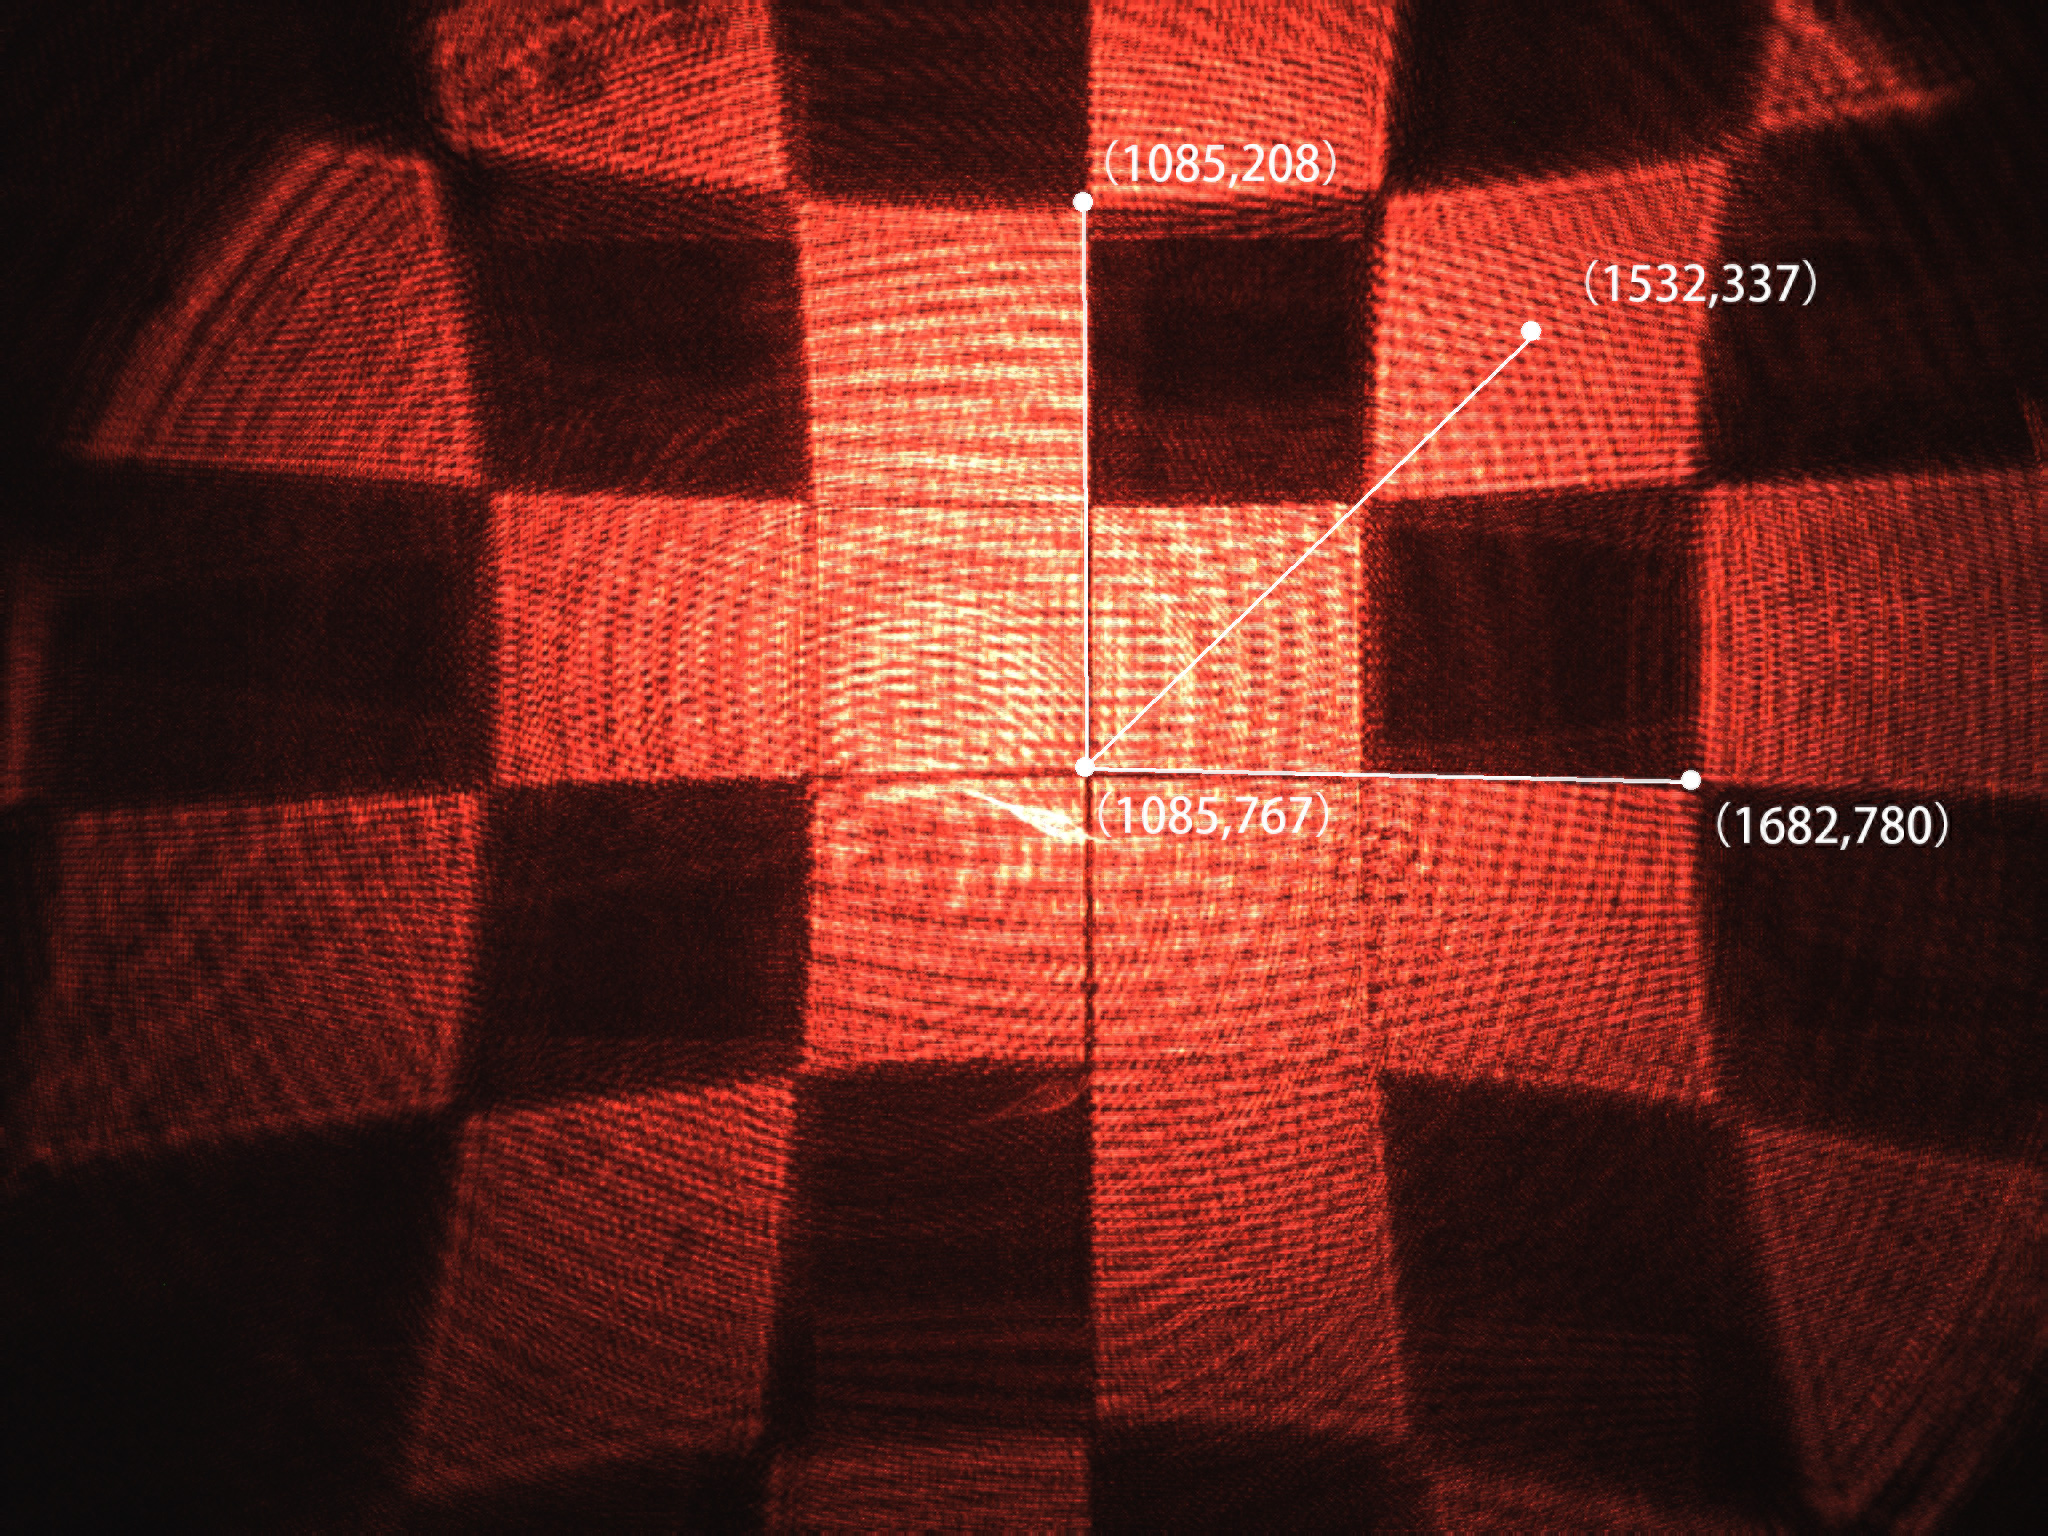
\includegraphics[width=0.3\textwidth]{C7_labeled/50_4_re.png}
		}
	\subfloat[$f=70mm$]{
		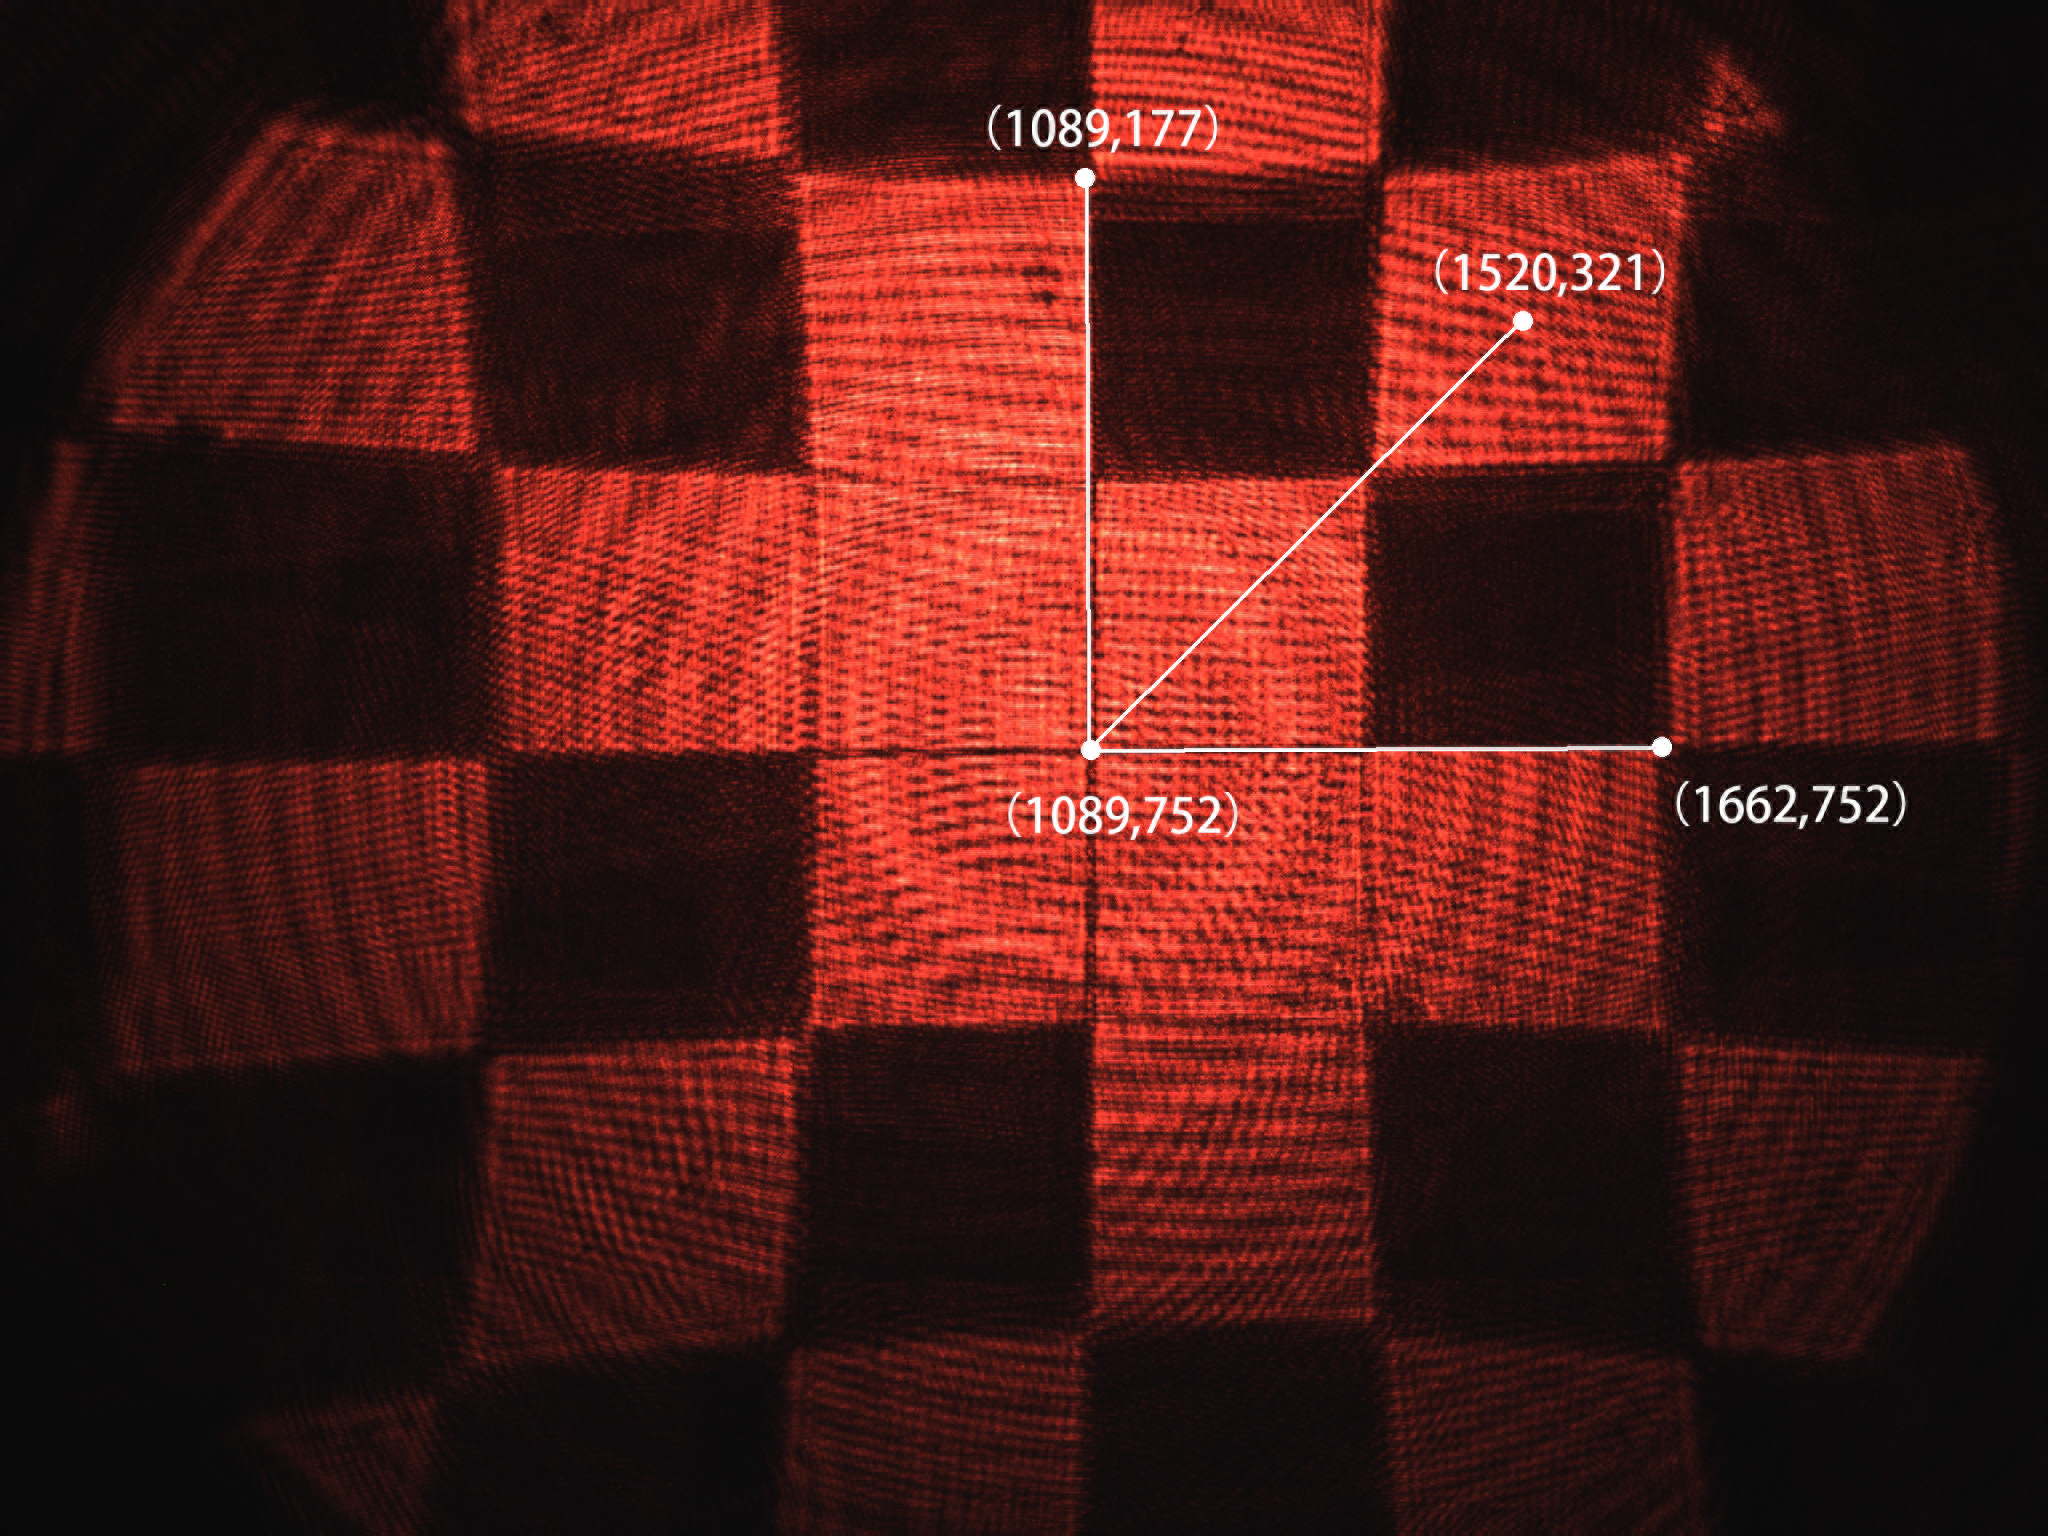
\includegraphics[width=0.3\textwidth]{C7_labeled/70_4.png}
		}
	\subfloat[$f=150mm$]{
		\includegraphics[width=0.3\textwidth]{C7_labeled/150_4.png}
		}
	\caption{不同焦距的透镜缩小4倍棋盘格畸变}
	\label{fig:dif_f}
\end{figure}

(2)拍摄同一透镜,不同缩小倍数棋盘格畸变的情况。
凸透镜焦距为 70mm,用 $6\times 8$ 或 $3\times 4$ 棋盘格,分别缩小 2、4、6 倍。

\begin{figure}[H]
	\centering
	\subfloat[2倍]{
	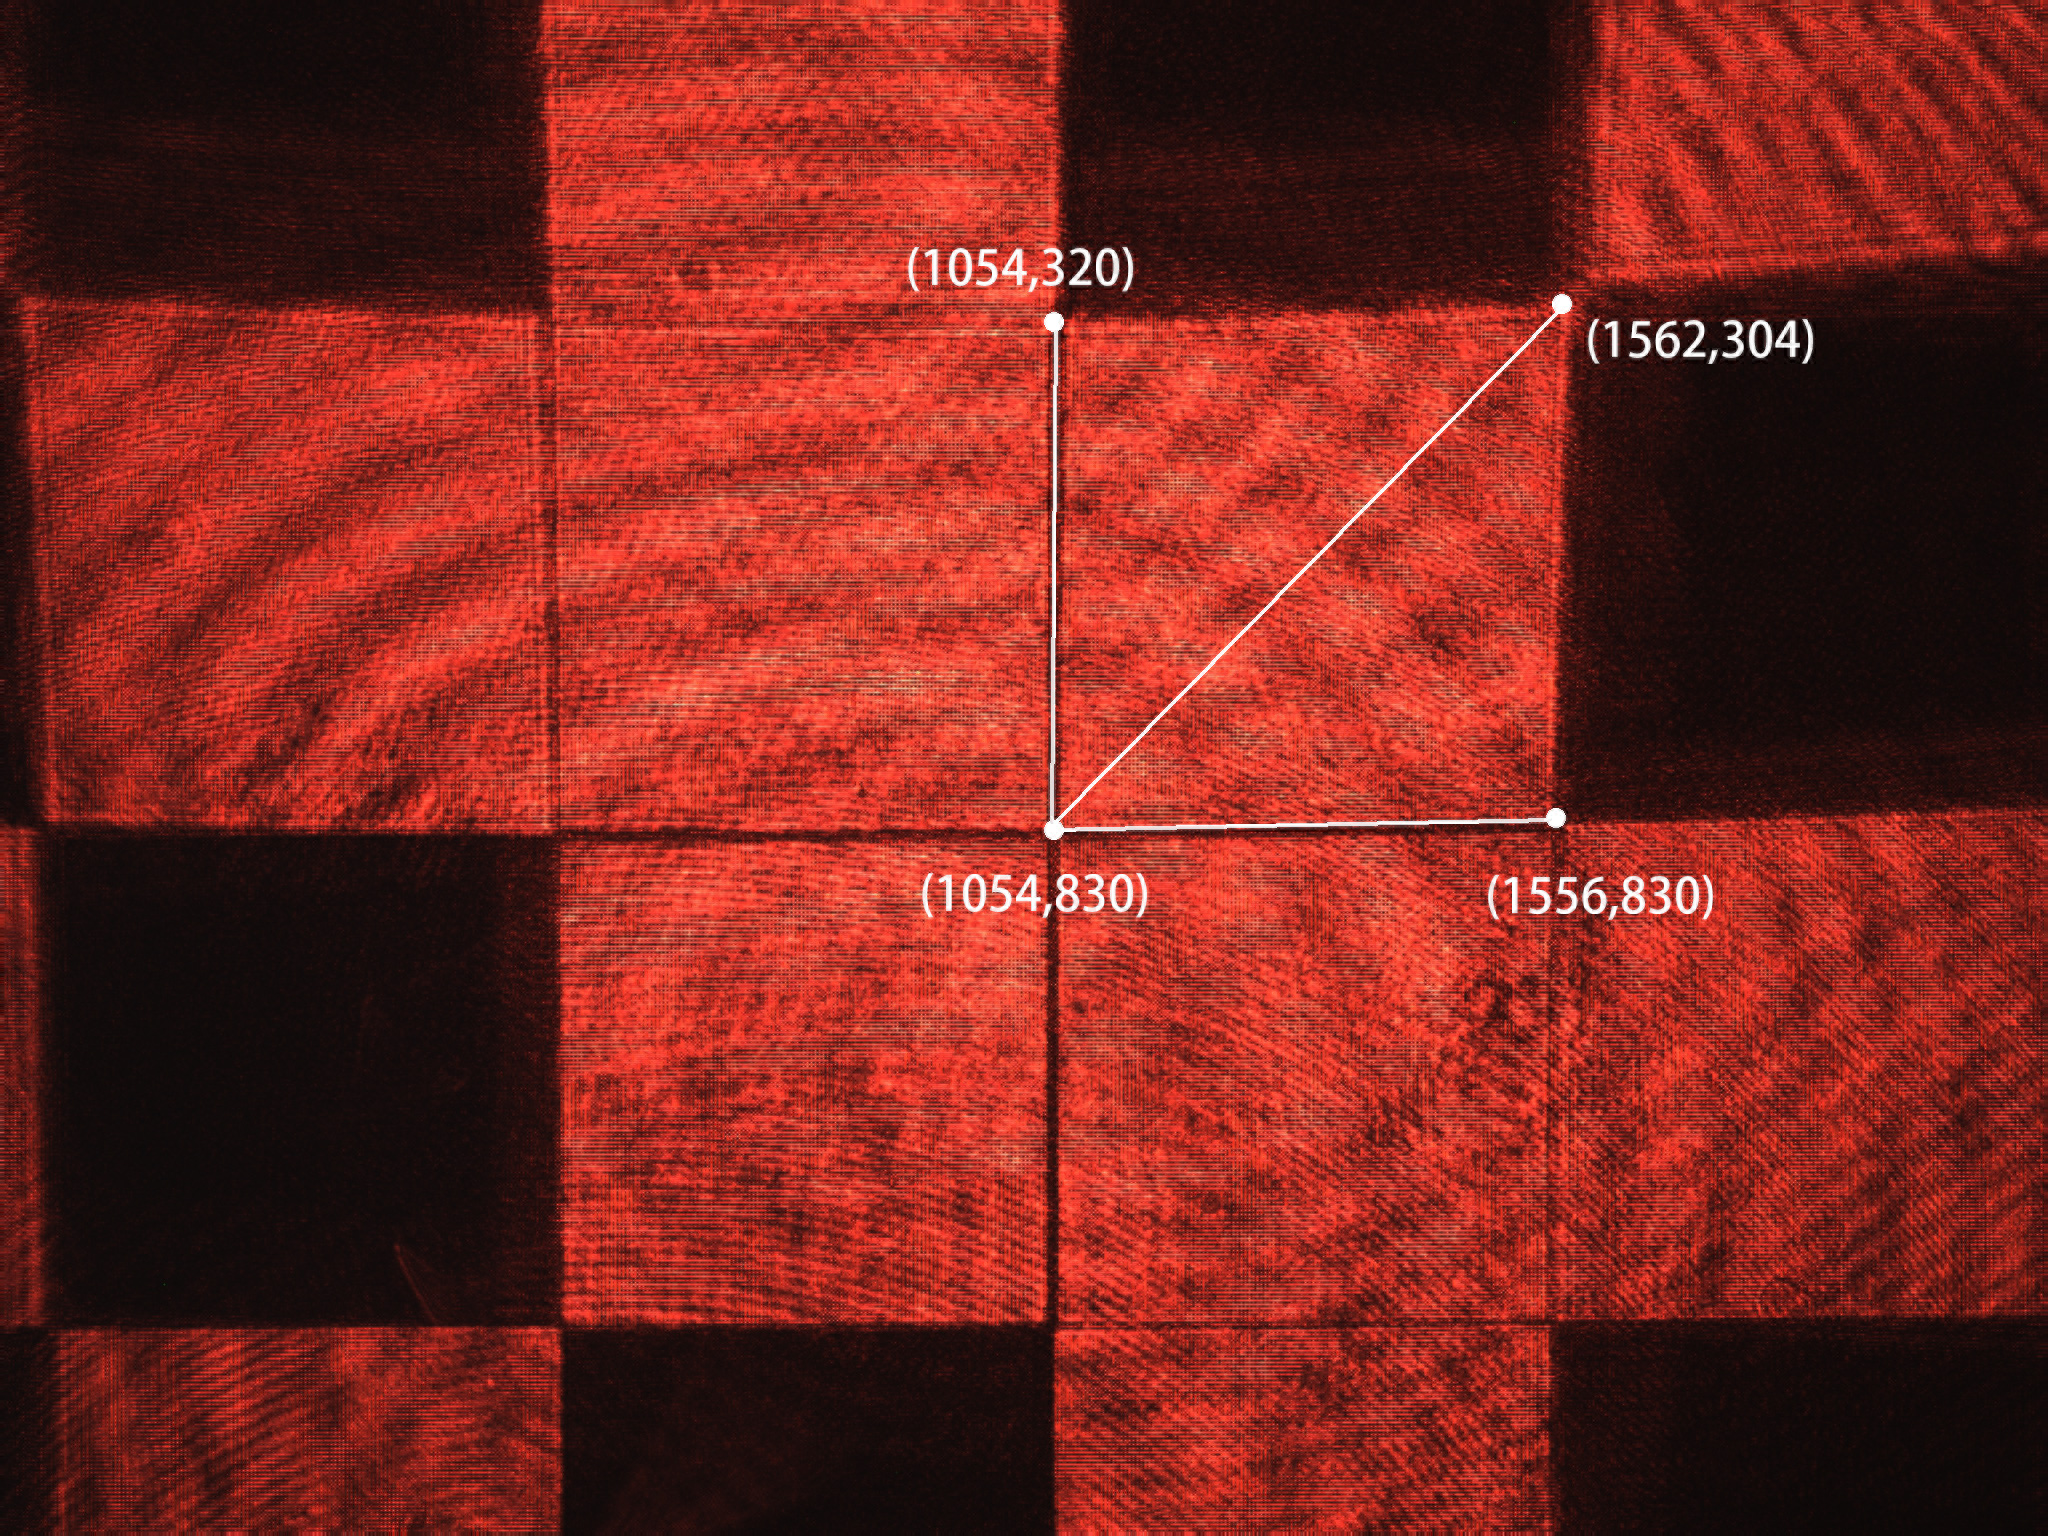
\includegraphics[width=0.3\textwidth]{C7_labeled/70_2.png}
	}%
	\subfloat[4倍]{
	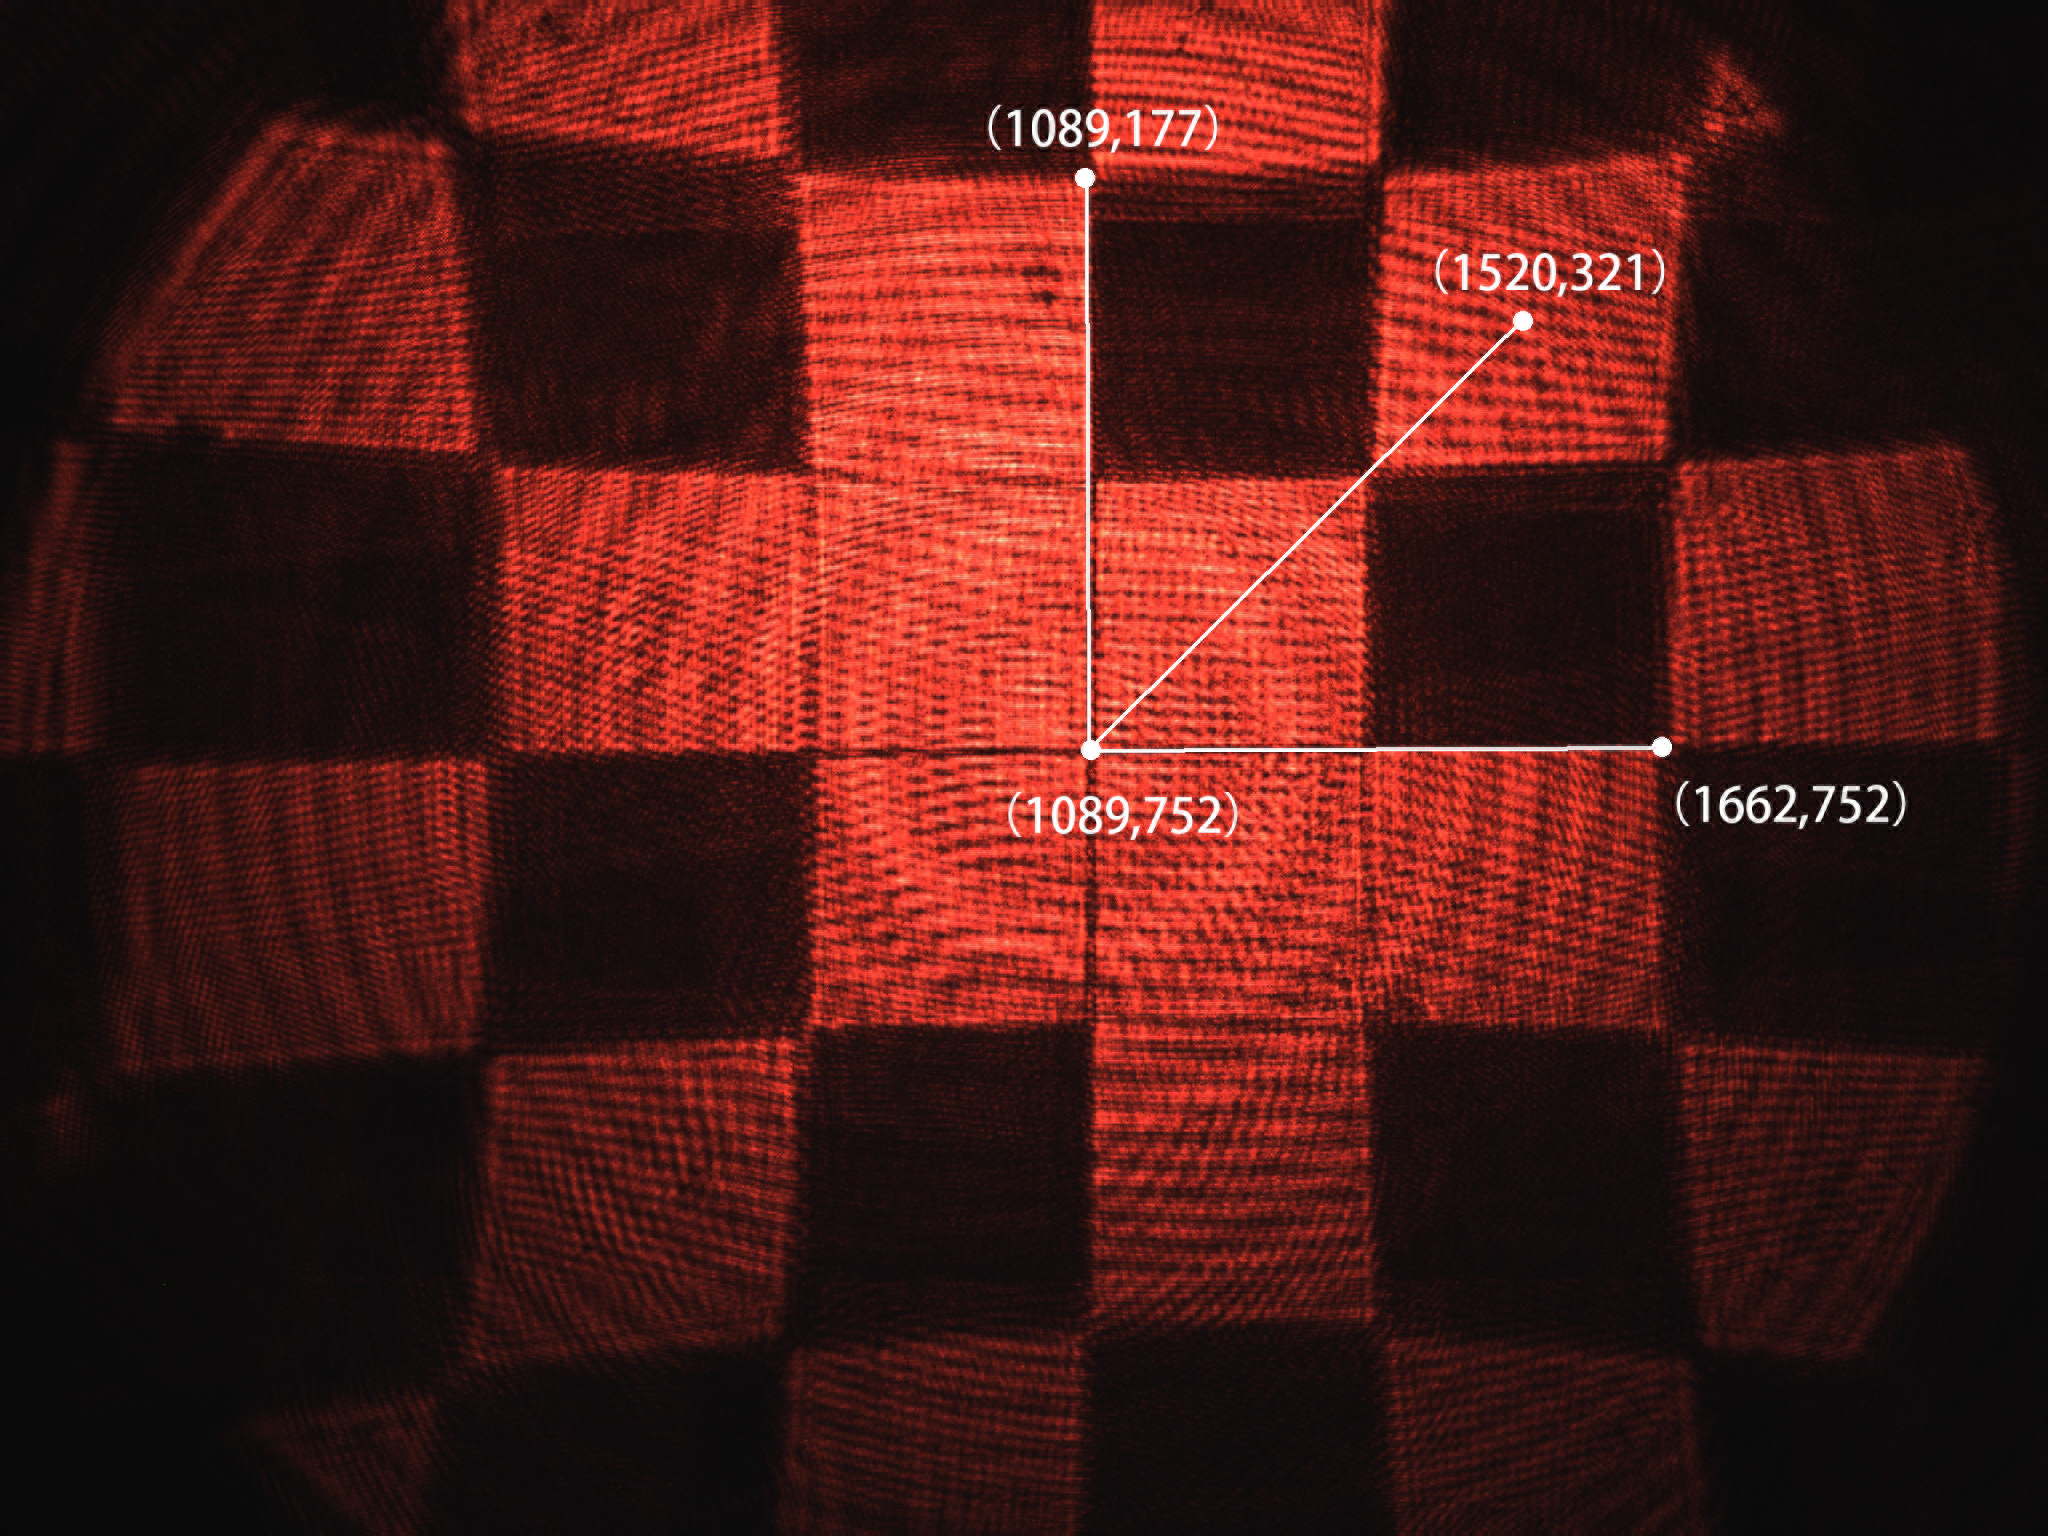
\includegraphics[width=0.3\textwidth]{C7_labeled/70_4.png}
	}%
	\subfloat[6倍]{
	\includegraphics[width=0.3\textwidth]{C7_labeled/70_6.png}
	}%
	\caption{相同焦距的透镜缩小不同倍数棋盘格畸变}
	\label{fig:dif_t}
\end{figure}

(3)拍摄同一透镜,不同放大倍数棋盘格畸变的情况。
选焦距70mm透镜,用 $48\times 64$ 棋盘格,分别放大 2 倍和 4 倍。
\begin{figure}[H]
	\centering
	\subfloat[2倍]{
	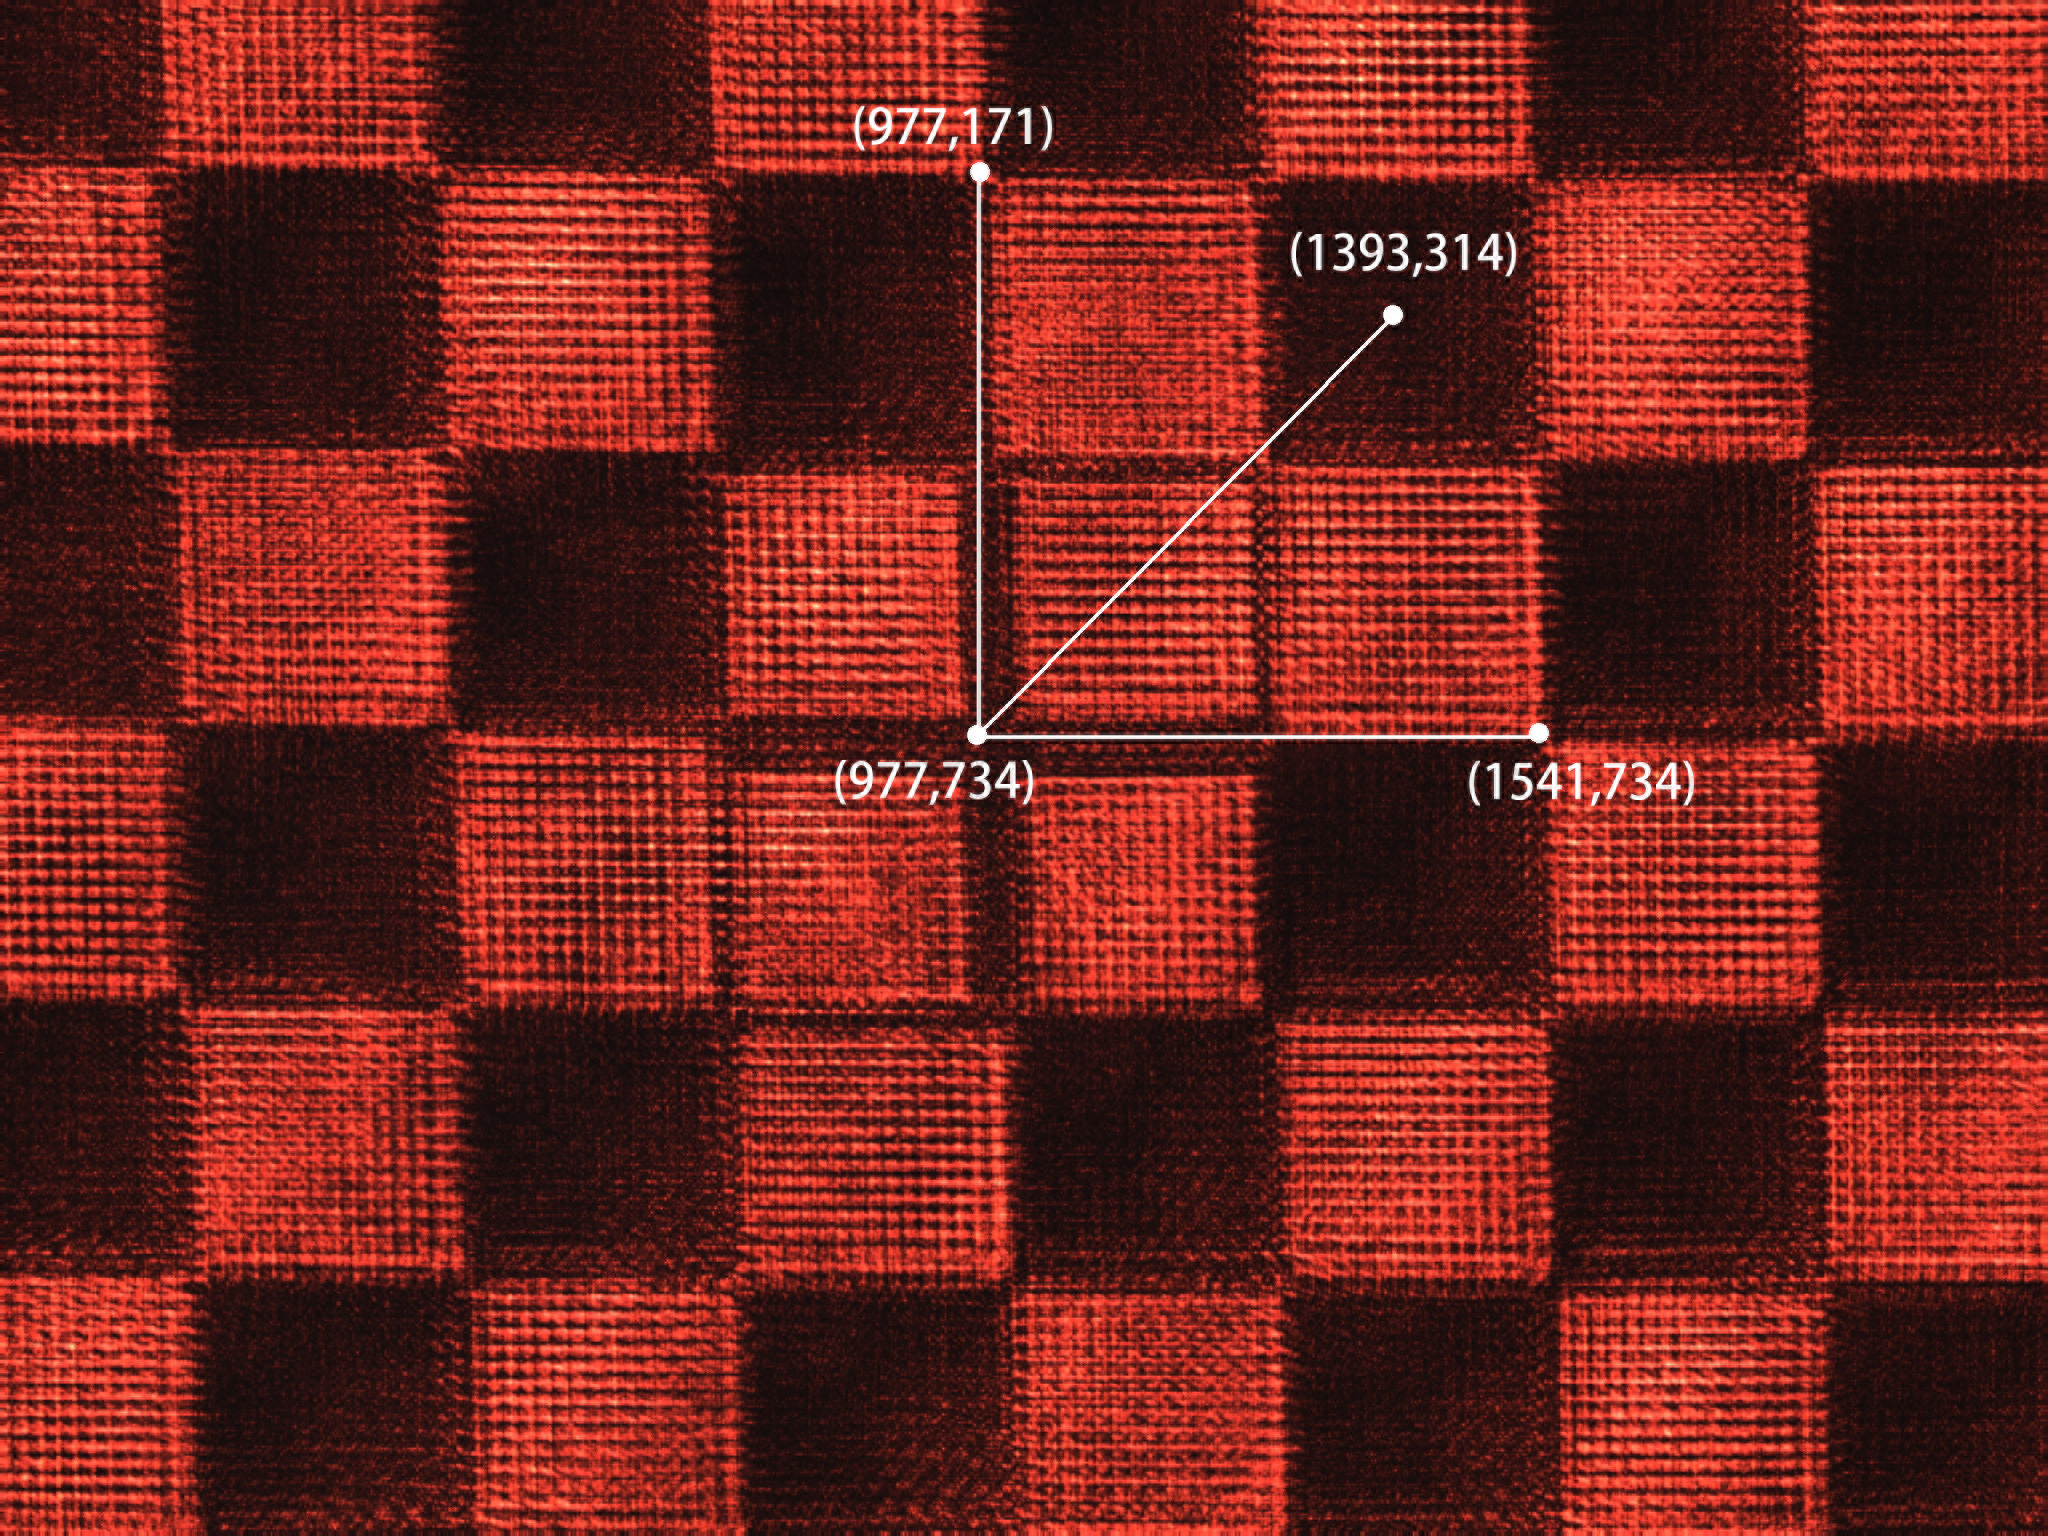
\includegraphics[width=0.3\textwidth]{C7_labeled/48x64_2X.png}
	}%
	\subfloat[4倍]{
	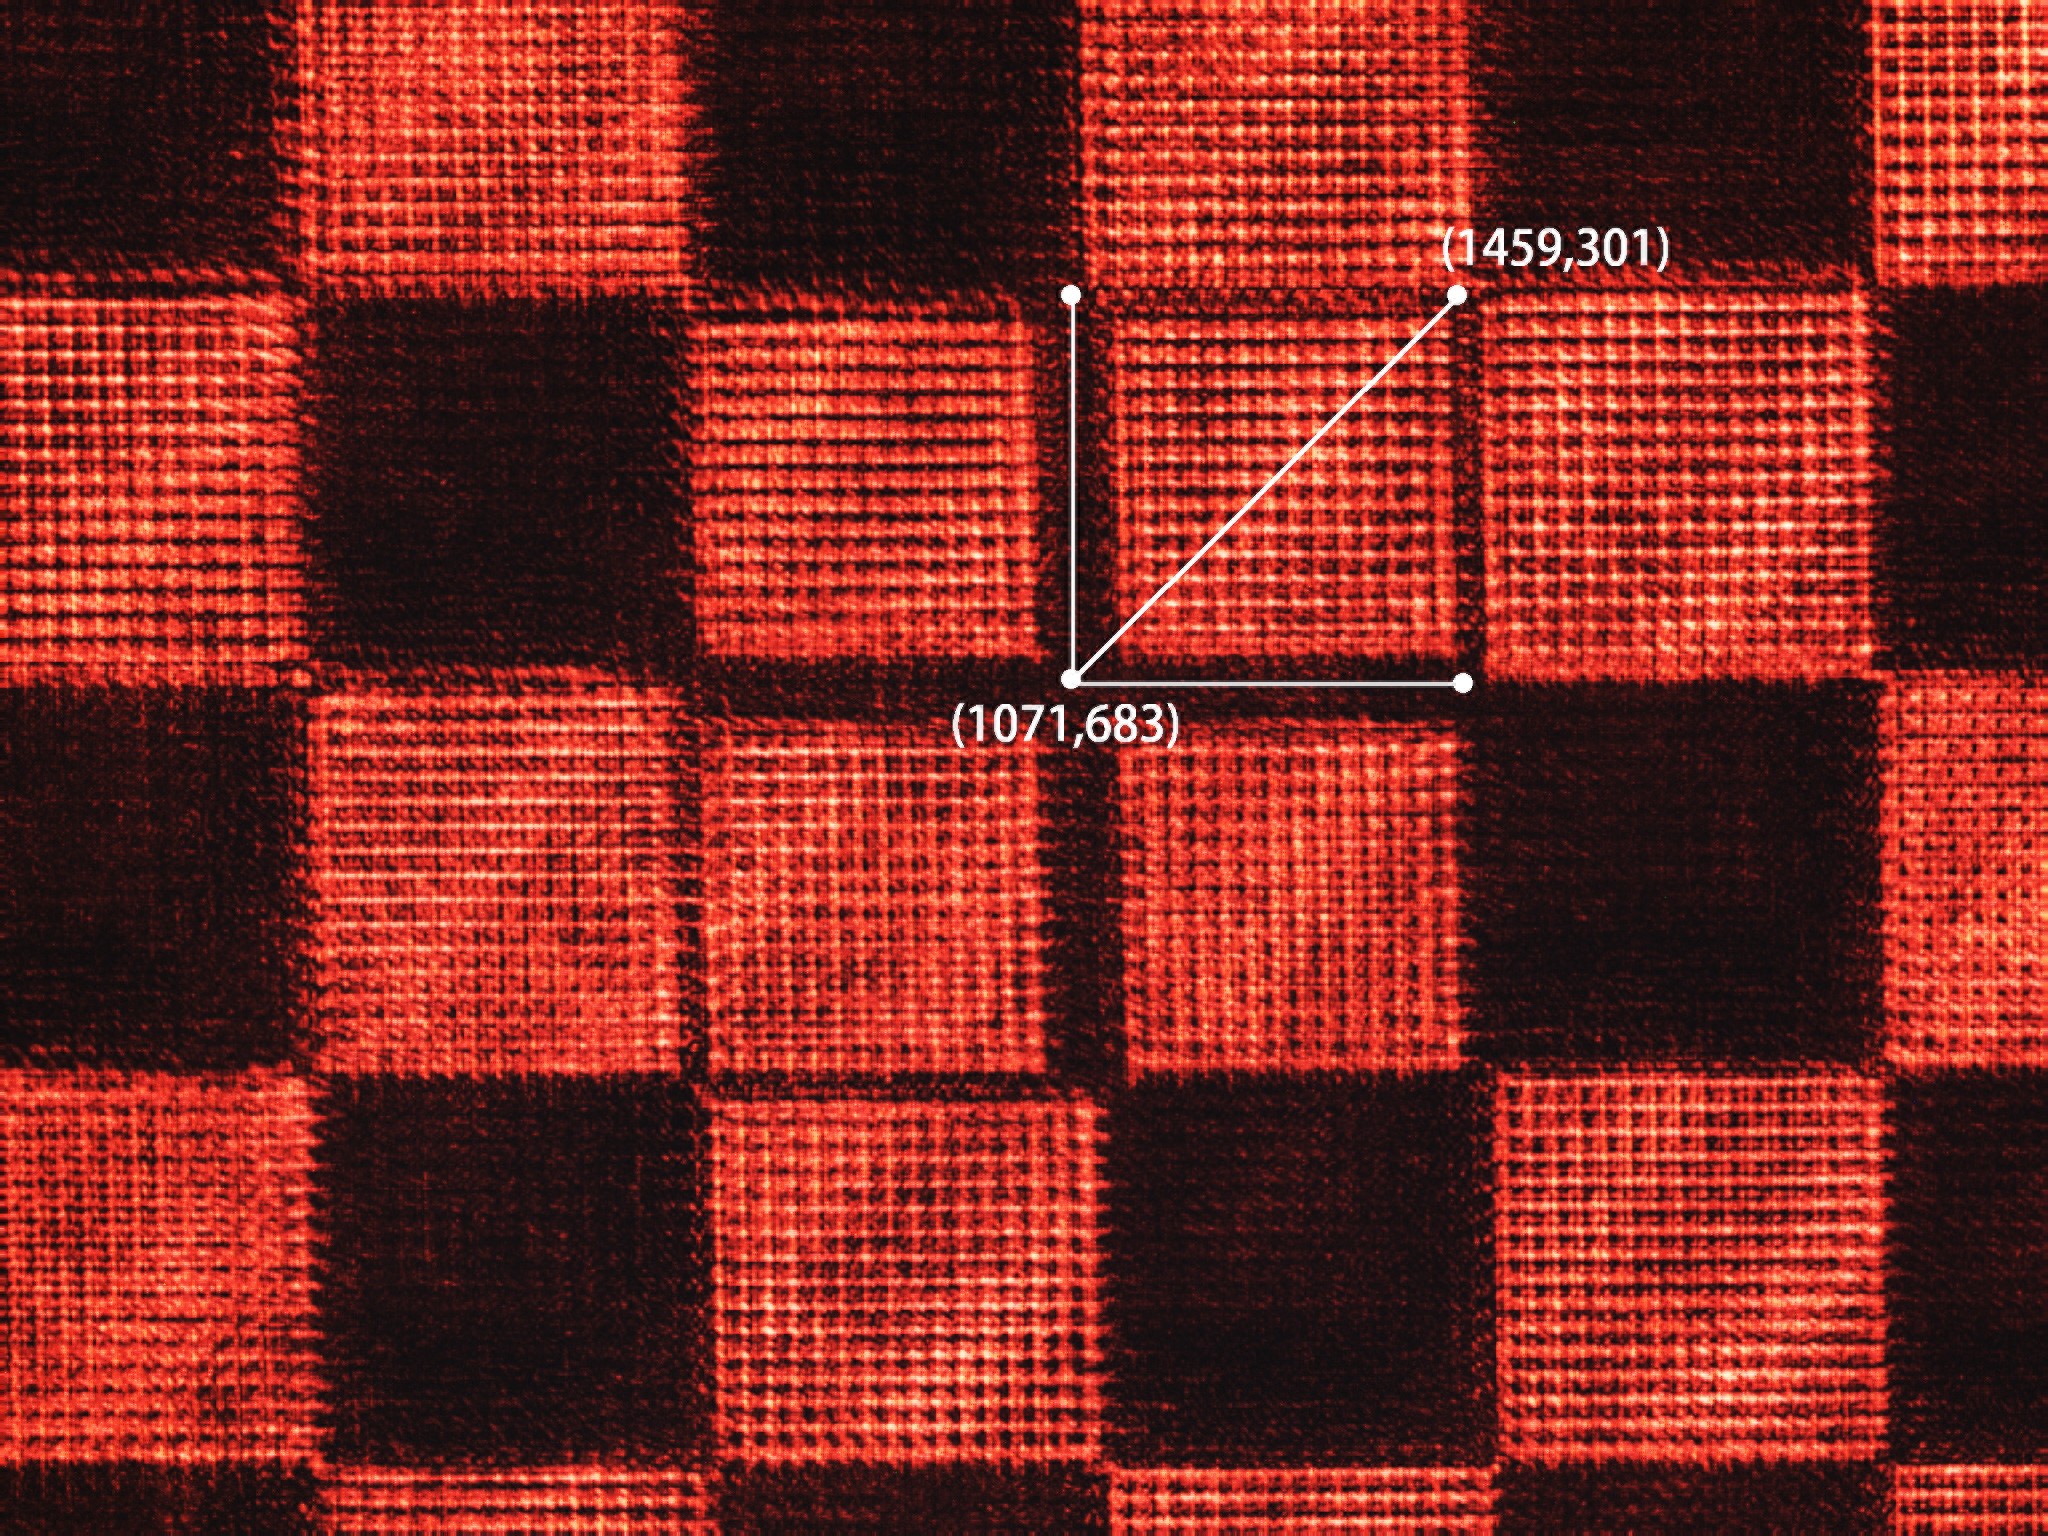
\includegraphics[width=0.3\textwidth]{C7_labeled/48x64_4X.png}
	}%
	\caption{焦距70mm透镜下缩小不同倍数$48\times64$棋盘格畸变}
	\label{fig:dif_t}
\end{figure}

处理实验数据,给出上述各种测量条件下的现对畸变值。结果见表\ref{tab:distortion}
\begin{table}[H]
	\centering
	  \begin{tabular}{ccccccc}
	  \toprule
	  棋盘格&透镜焦距f/mm & 放大倍数 &x方向畸变 & y方向畸变 & xy方向水平畸变 & xy方向垂直畸变  \\
	  \midrule
	  $6\times 8 $ & 150   & 0.25 &0.19\% & 1.35\% & 0.00\% & -2.05\% \\
	  & 70    & 0.25&10.19\% & 10.58\% & 10.51\% & 10.51\% \\
	  & 50    & 0.25 &14.81\% & 7.50\% & 14.62\% & 10.26\% \\
	  & 70    & 0.5  &-3.46\% & -1.92\% & -2.31\% & 1.15\% \\
	  & 70    & 0.166&17.30\% & 8.61\% & 18.16\% & 15.46\% \\
	  \midrule
	  $48\times 64 $ & 70    & 2 &8.46\% & 8.27\% & 6.67\% & 7.69\% \\
	  & 70    & 4  &-25.38\% & -26.54\% & -25.38\% & -26.54\% \\
	  \bottomrule
	  \end{tabular}
	\caption{畸变}
	\label{tab:distortion}
  \end{table}
  
由CCD拍摄的图像可以看出,上述三个焦距均发生枕形畸变。
分析上述数据,发现成像中距离中心位置越近的点畸变越小,距离中心位置越远的点畸变越大,这与傍轴近似的分析是一致的。
同一焦距同一放大倍数所对应的相同距离不同方向的四个点的畸变值有差异,水平方向与竖直方向的畸变值不同,这说明对于每个透镜组成的光学系统而言,并不是完全球对称,实验光路存在一定偏差。
在相同的放大倍数时,透镜焦距越大,畸变率越小;在相同的焦距情况下,放大倍数越小,畸变越明显。畸变与镜头的广角有关,视场角越大,畸变越明显,这与理论分析是一致的。
对比不同放大倍数的同一点的畸变值可以发现,放大倍数较大的透镜所得的畸变值相对来说较大,与事实规律相符。
放大两倍的畸变值远远大于缩小相同倍数的畸变值,放大时物距小,实验时因物距偏差造成的实验误差可能比较大。

\subsection{空间频谱和滤波实验}
\subsubsection{验证阿贝成像原理(一)}
用CCD放置于傅氏面,观察傅氏面P2的频谱样式,并手描记录衍射光点的分布,如图\ref{fig:ab1_raw}.
\begin{figure}[H]
	\centering
	\includegraphics[width=0.4\textwidth]{C7.2/1/raw.png}
	\caption{傅氏面$P_2$的频谱样式}
	\label{fig:ab1_raw}
\end{figure}

观察到横向排列的亮度不同的点阵,
即为光栅的夫琅禾费衍射图。光轴上的一点
是 0 级衍射,其他依次为$\pm 1$、$\pm 2$级衍射。从傅里叶光学来看,这些光点正好
对应于各傅里叶分量。0 级为直流分量,$\pm 1$
级为基频分量,$\pm 2$ 级为倍频分量。

调节底座位置和狭缝宽度的大小使 0 级光点刚好通过狭缝,档去 0 级以外的各光点,观察 P 平面上的图形,检
查是否有干涉条纹。增大狭缝宽度,使 0 级和$\pm 1$ 级光点通过,观察 P 平面上所成的像。再逐渐增大狭缝宽度
直至完全拿开狭缝,逐次让更高级次的光点通过,分别观察并记录成像的特点及条纹间距。
\begin{figure}[H]
	\centering
	\subfloat[0级]{
	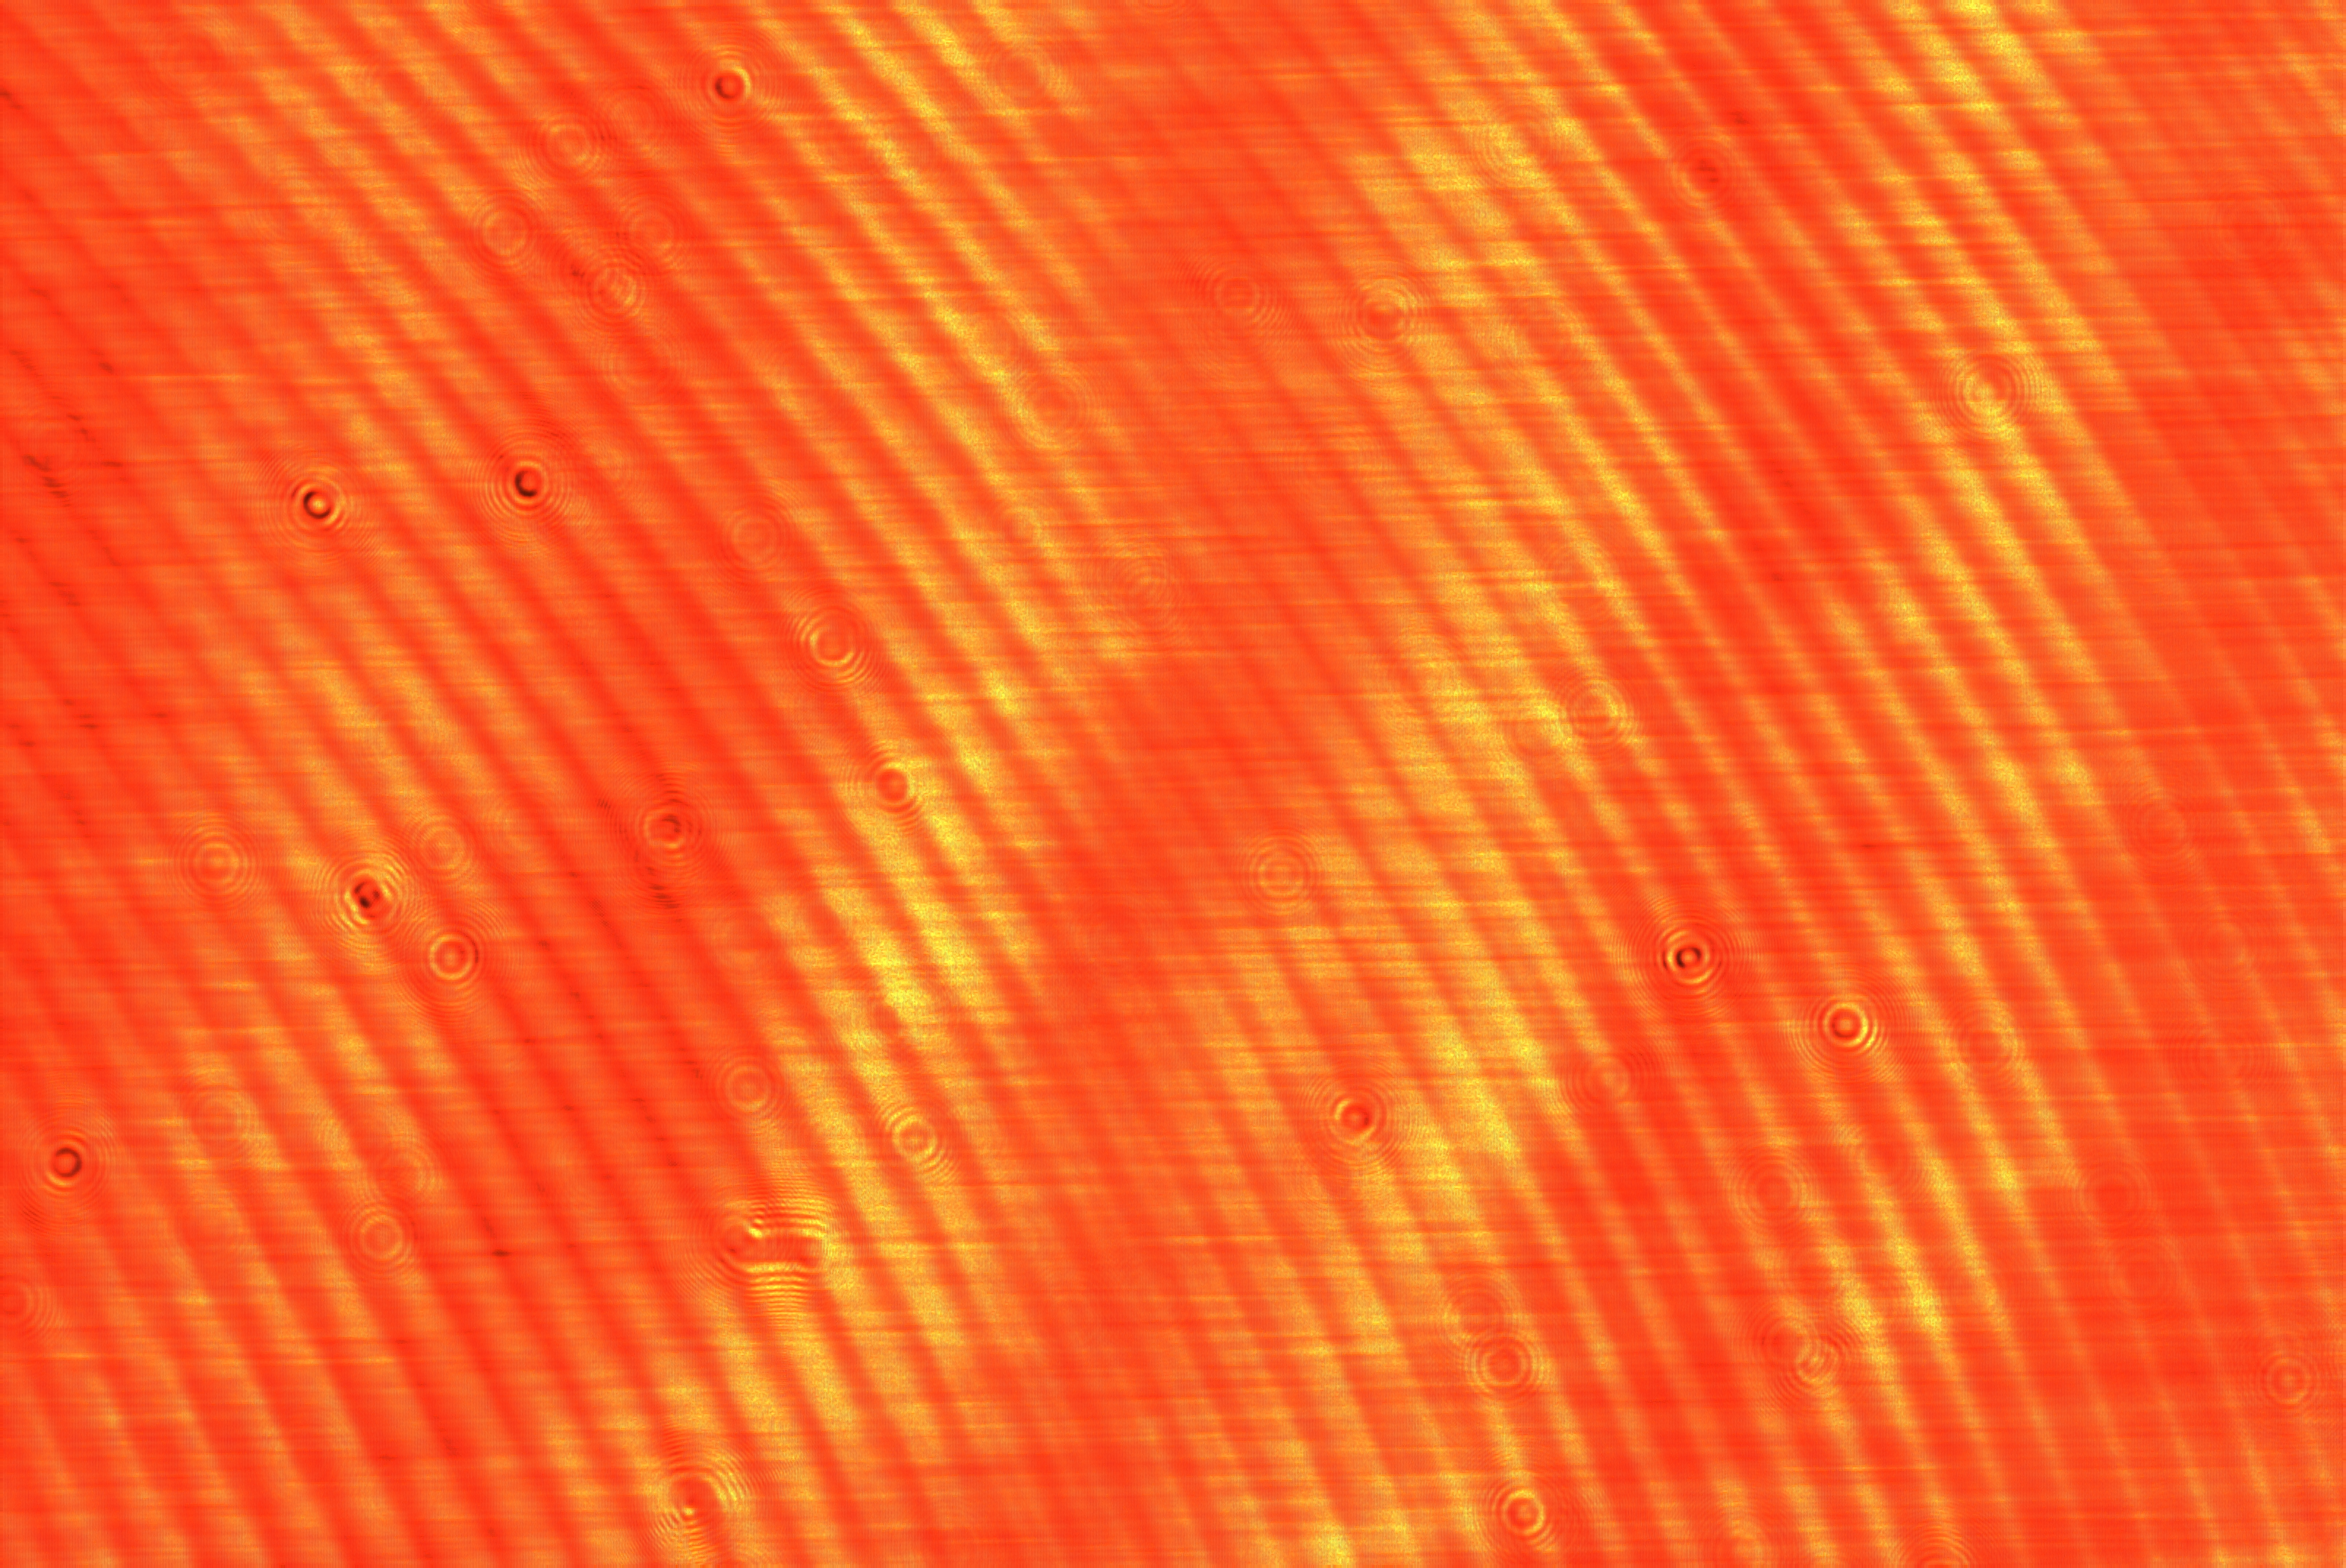
\includegraphics[width=0.3\textwidth]{C7.2/1/0.png}
	}%
	\subfloat[1级]{
	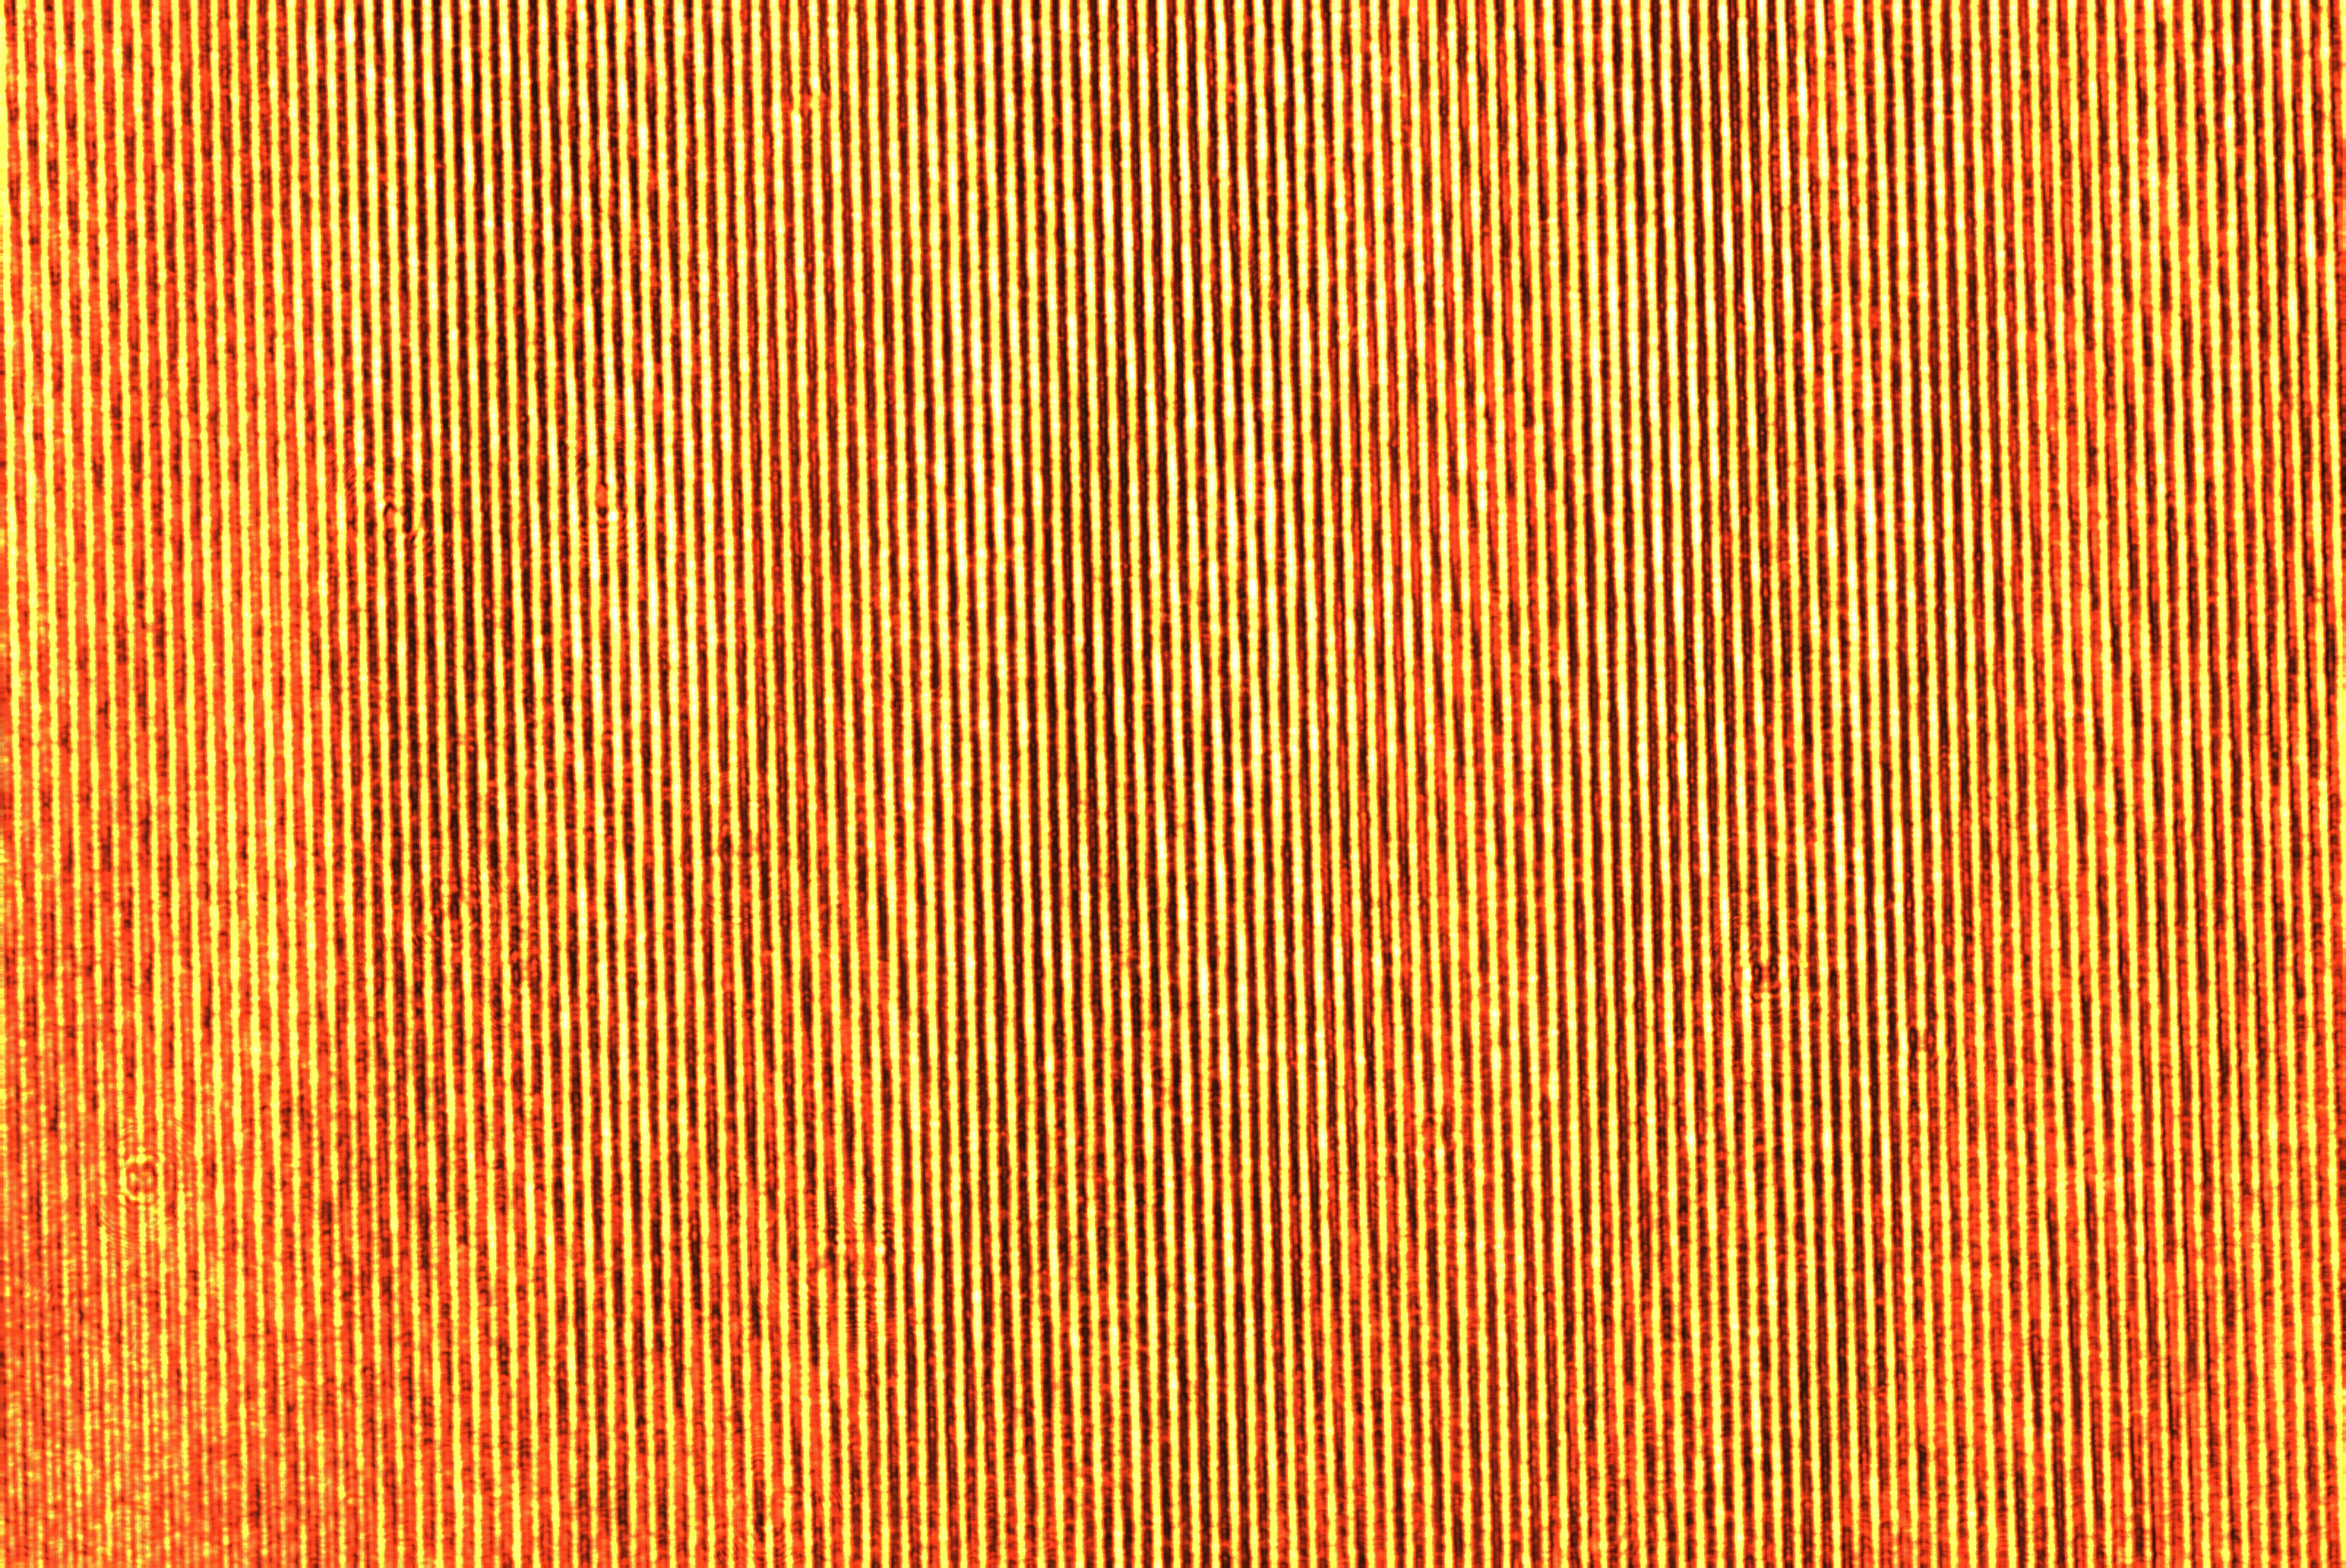
\includegraphics[width=0.3\textwidth]{C7.2/1/01.png}
	}%

	\subfloat[2级]{
		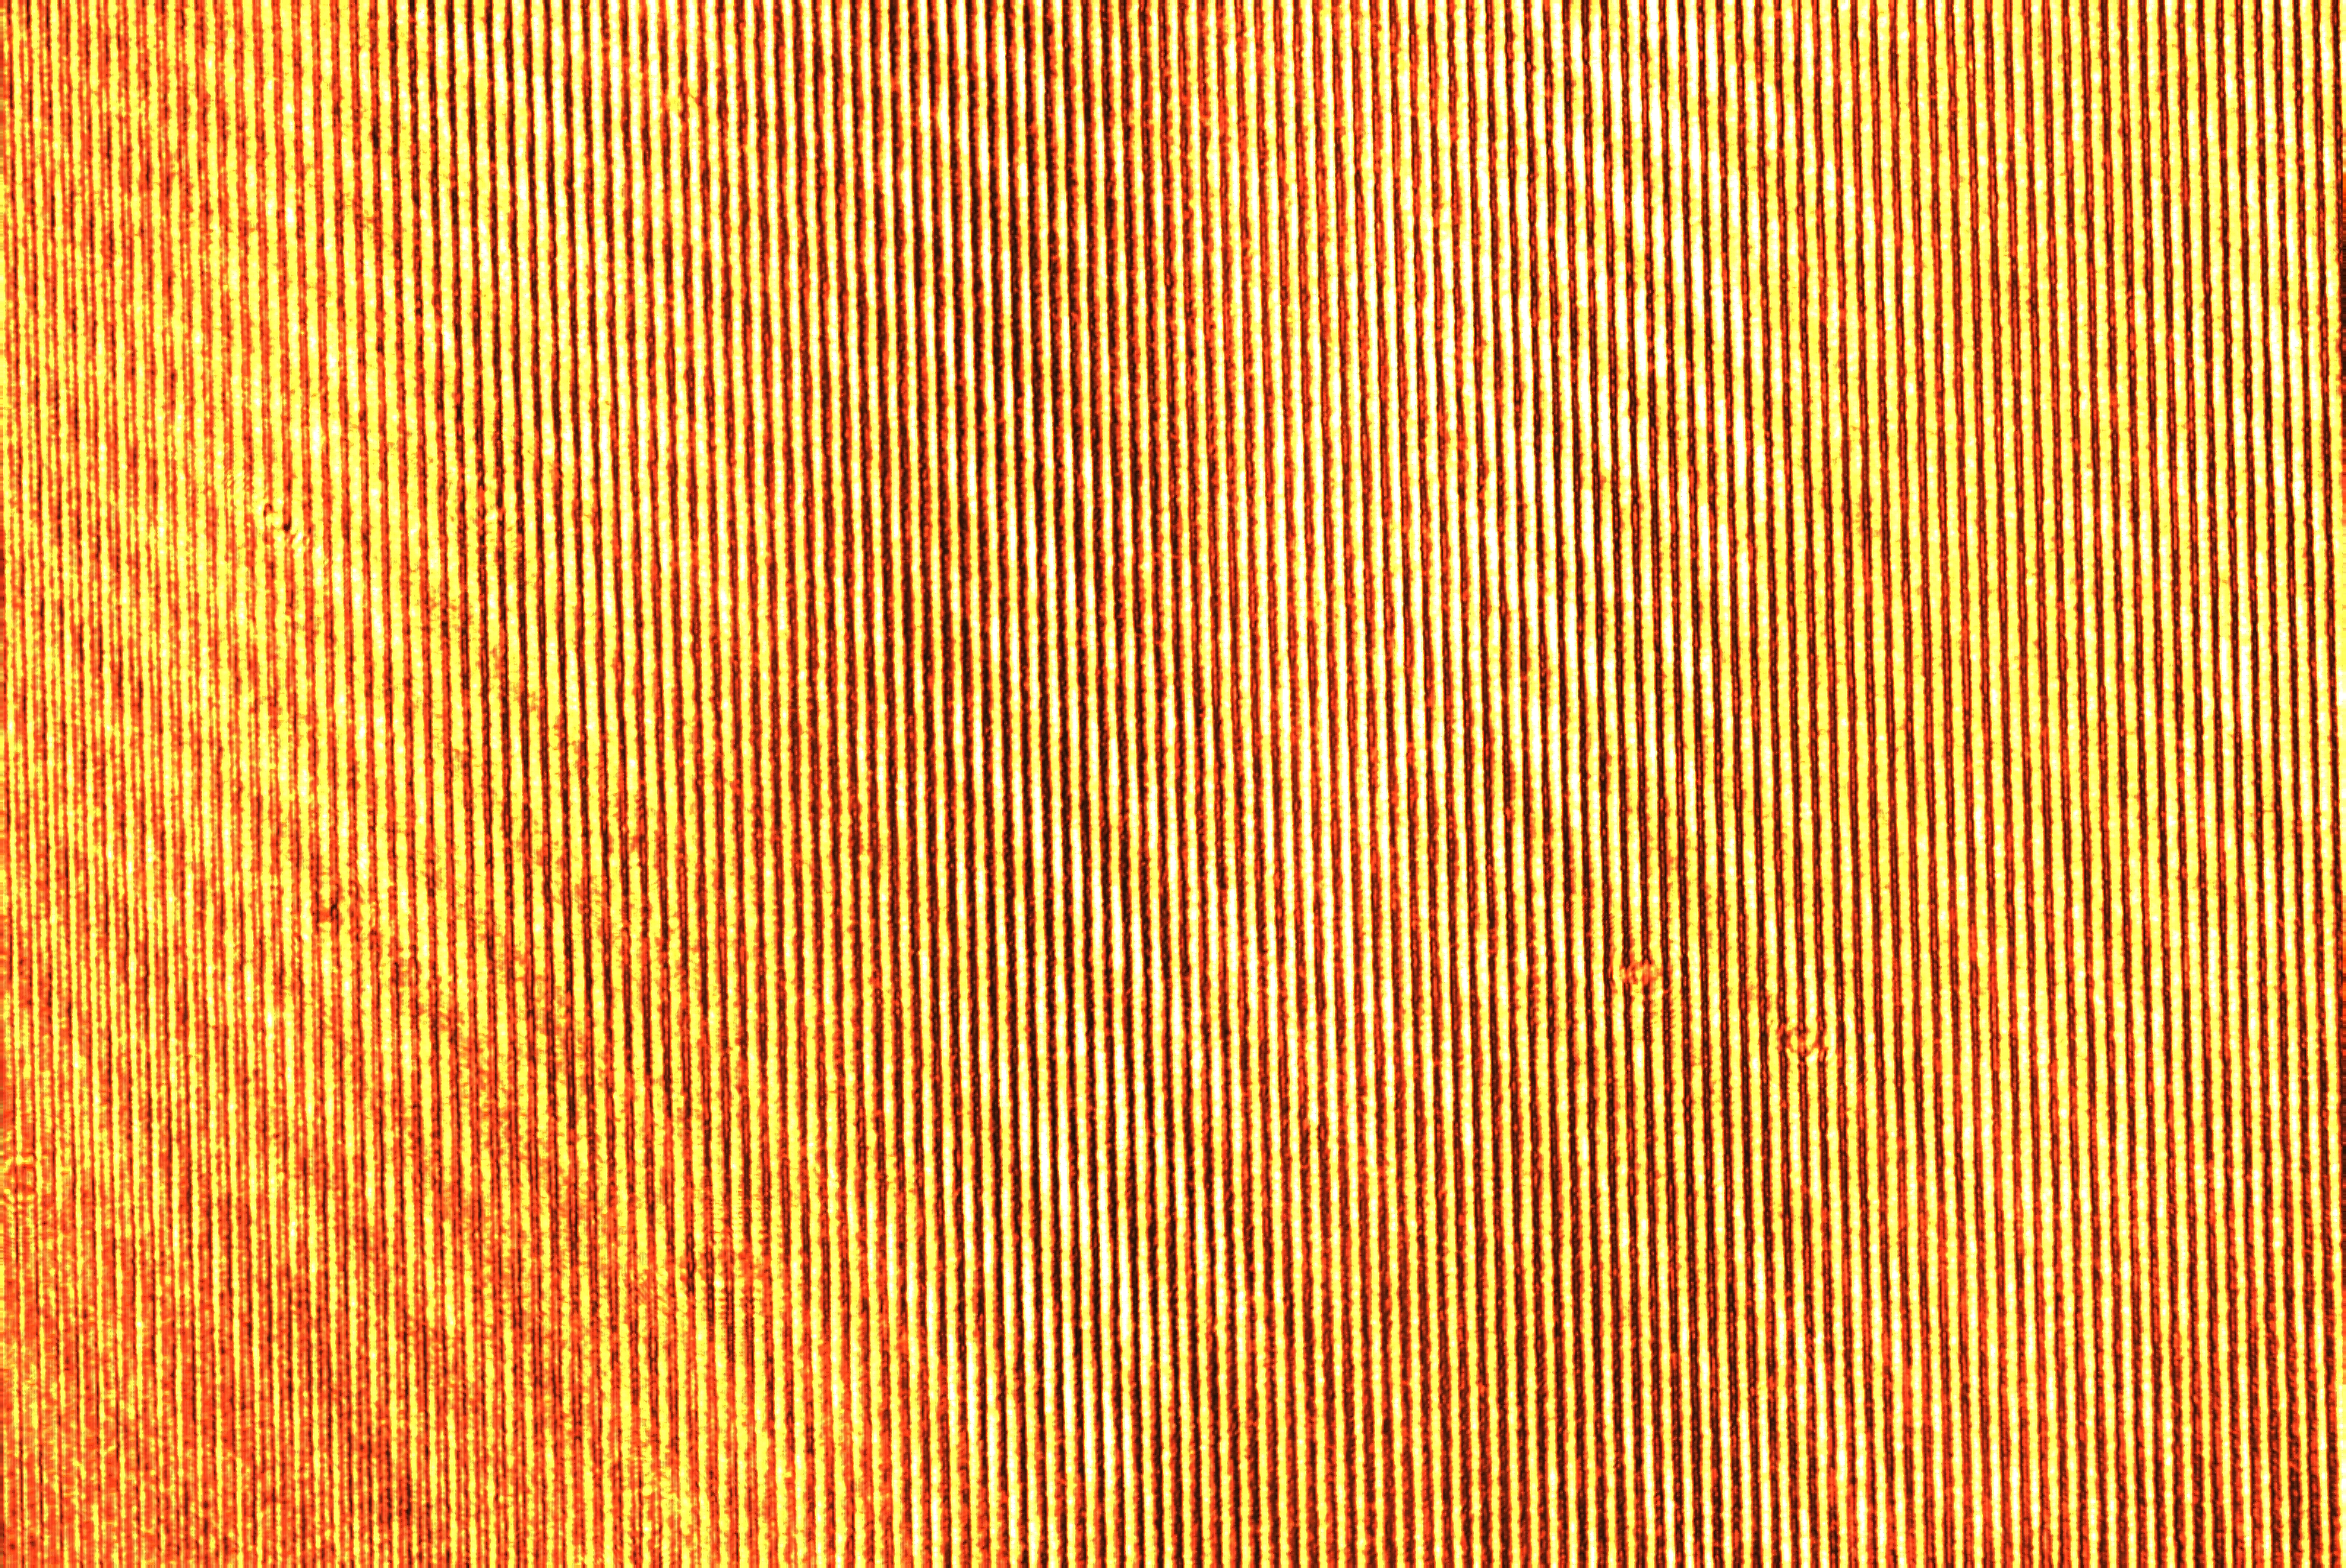
\includegraphics[width=0.3\textwidth]{C7.2/1/02.png}
	}%
	\subfloat[无狭缝]{
	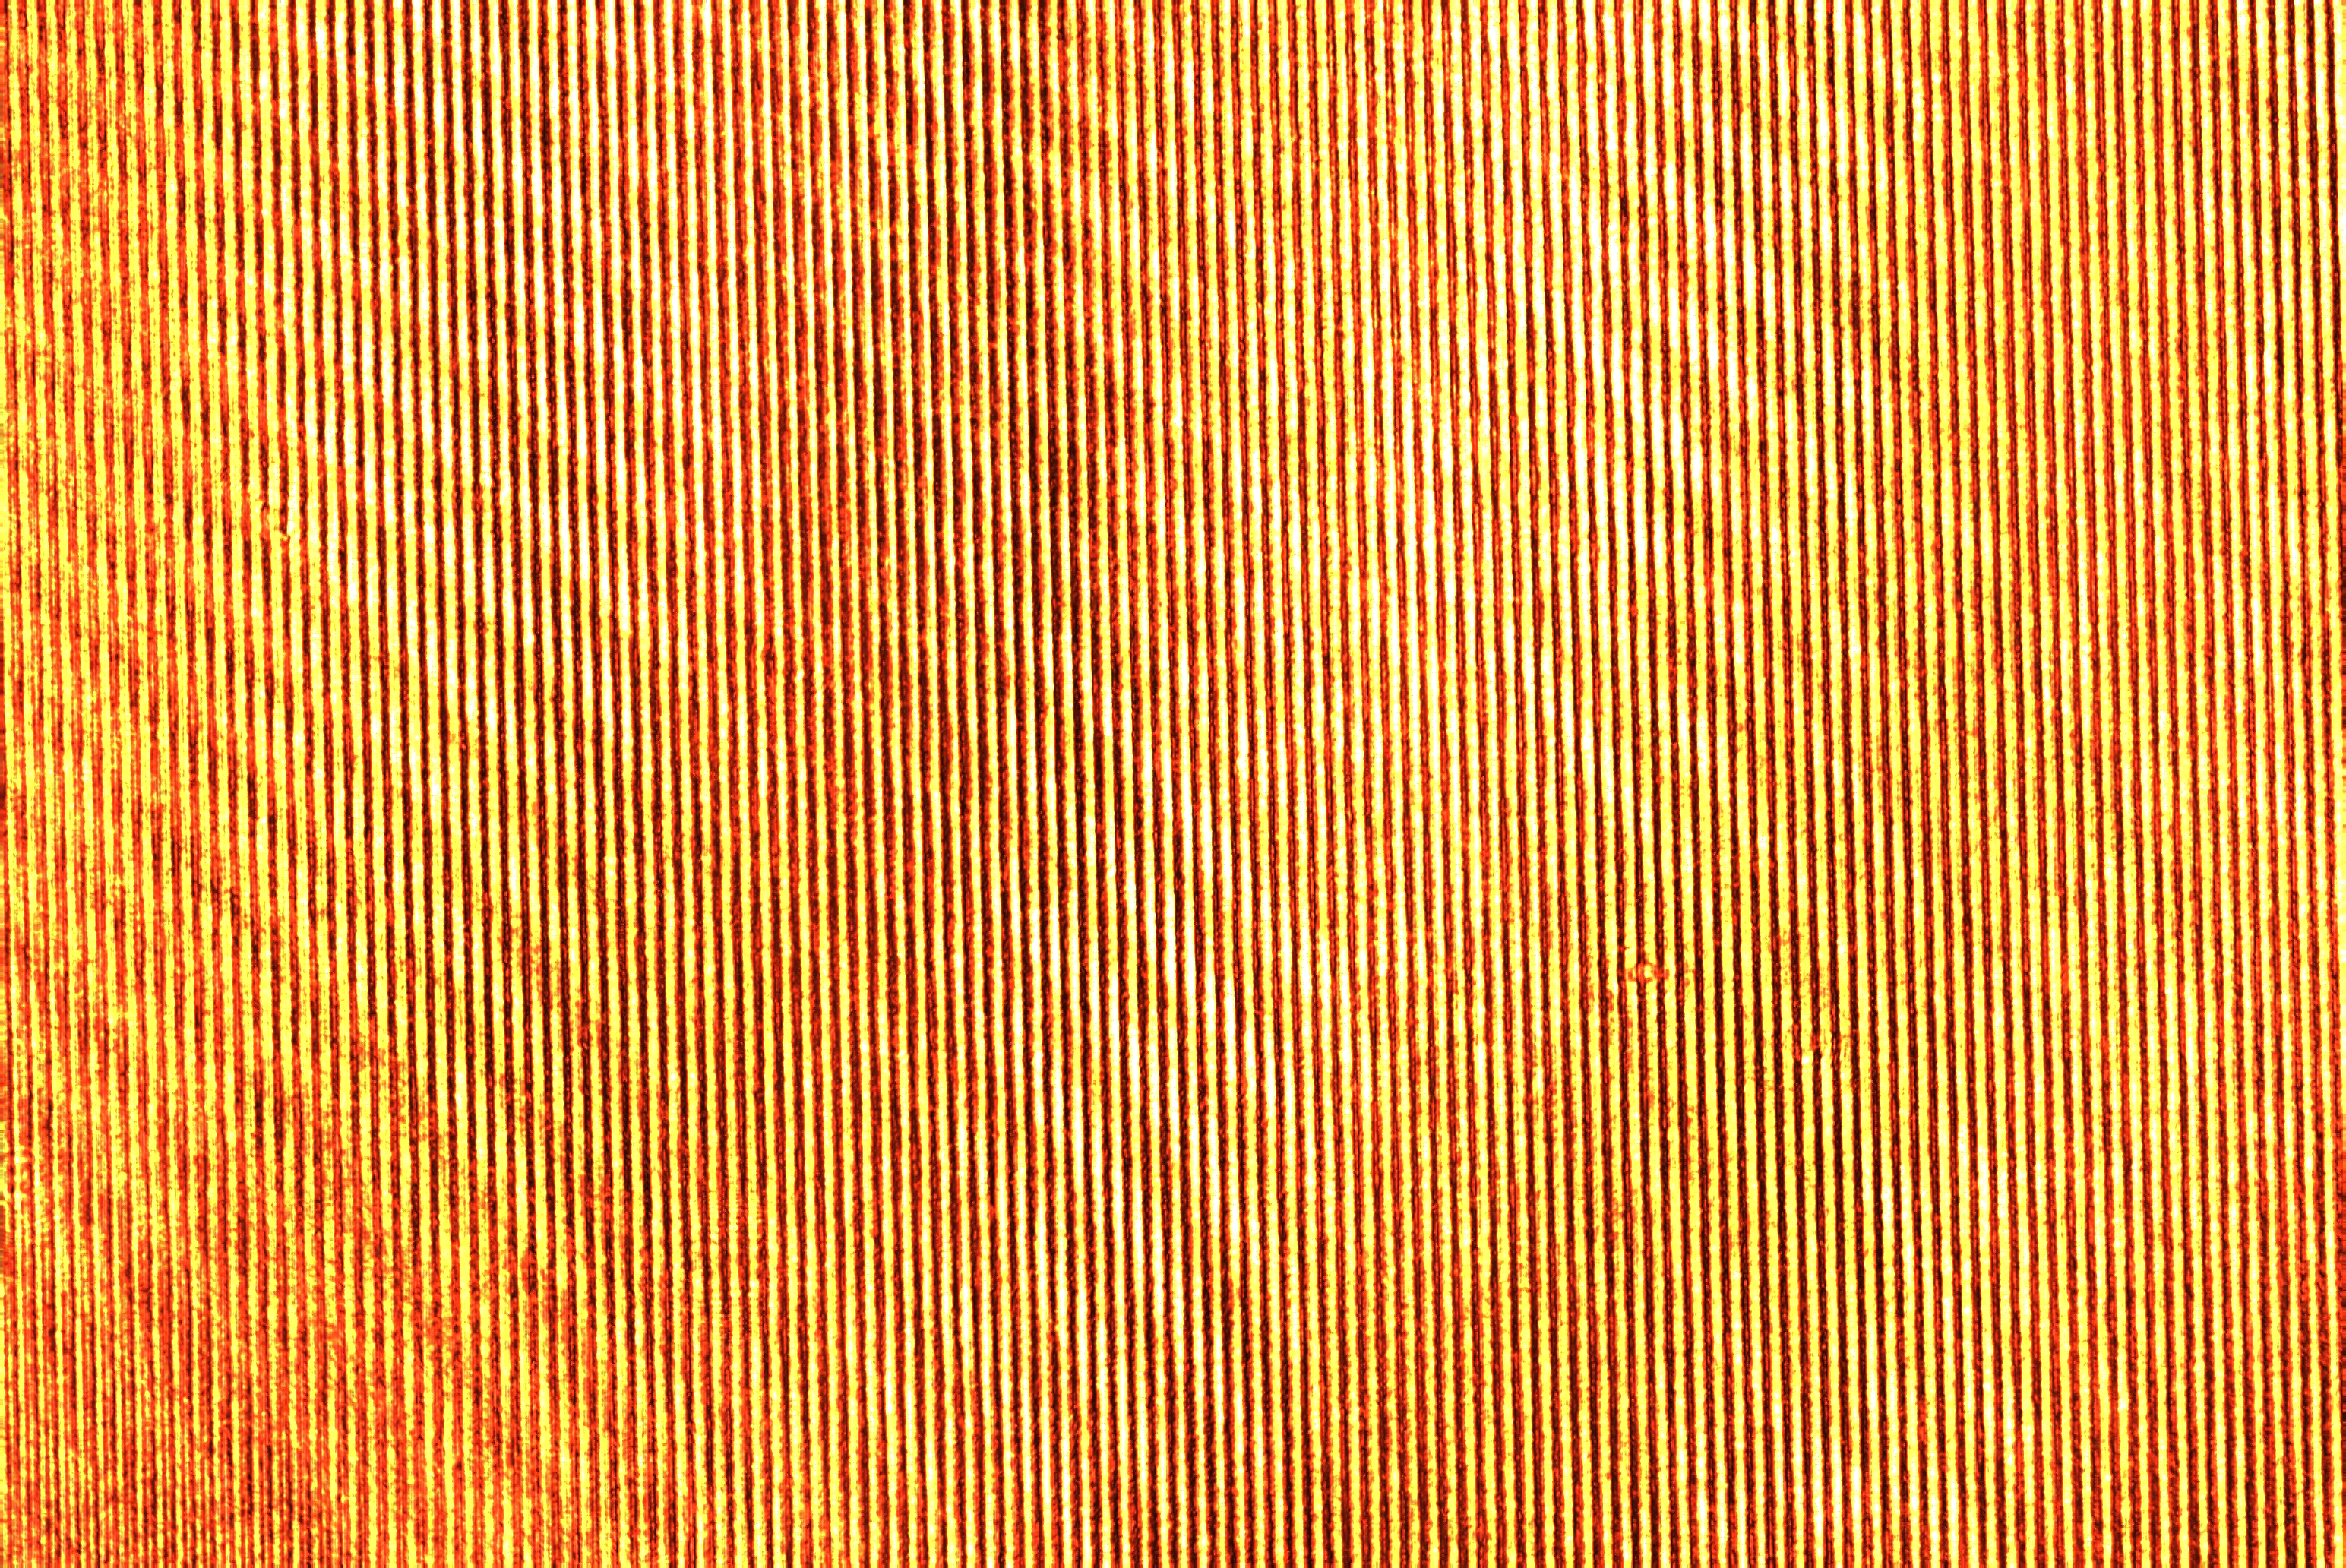
\includegraphics[width=0.3\textwidth]{C7.2/1/none.png}
	}%
	\caption{实物光栅衍射成像}
	\label{fig:ab1}
\end{figure}

刚好使 0 级光点通过时,用 CCD
在像平面上拍摄并观察,可知像面上是一个
照度基本均匀,没有条纹图案,这是因为 0
级光点处聚集的是类似“直流量”的分量,
在像平面上反映为一个均匀的光照,故用
CCD 观察没有光栅的图案。增大狭缝宽度,
使 0 级和$\pm 1$ 级光点通过,开始观察到有条
纹出现。随着增大狭缝宽度,高频信息得以通
过,最终在像平面上观察到像和光栅基本相
同,在这一过程,像平面观察的图案表现为可分辨的条纹
数增加,条纹间距减小,分辨率增高,图案
细节趋于完整。

\subsubsection{验证阿贝成像原理(二)}
加载像原理和空间滤波实验”中的“128T 一维光栅”图\ref{fig:ab2_raw1}至空间光
调制器,仔细观察傅氏面$P_2$的频谱样式,如图\ref{fig:ab2_raw2}.
\begin{figure}[H]
	\centering
	\subfloat[128T 一维光栅]{\label{fig:ab2_raw1}
	\includegraphics[width=0.3\textwidth]{C7.2/2/128T一维光栅.png}
	}%
	\subfloat[傅氏面 $P_2$的频谱样式]{\label{fig:ab2_raw2}
	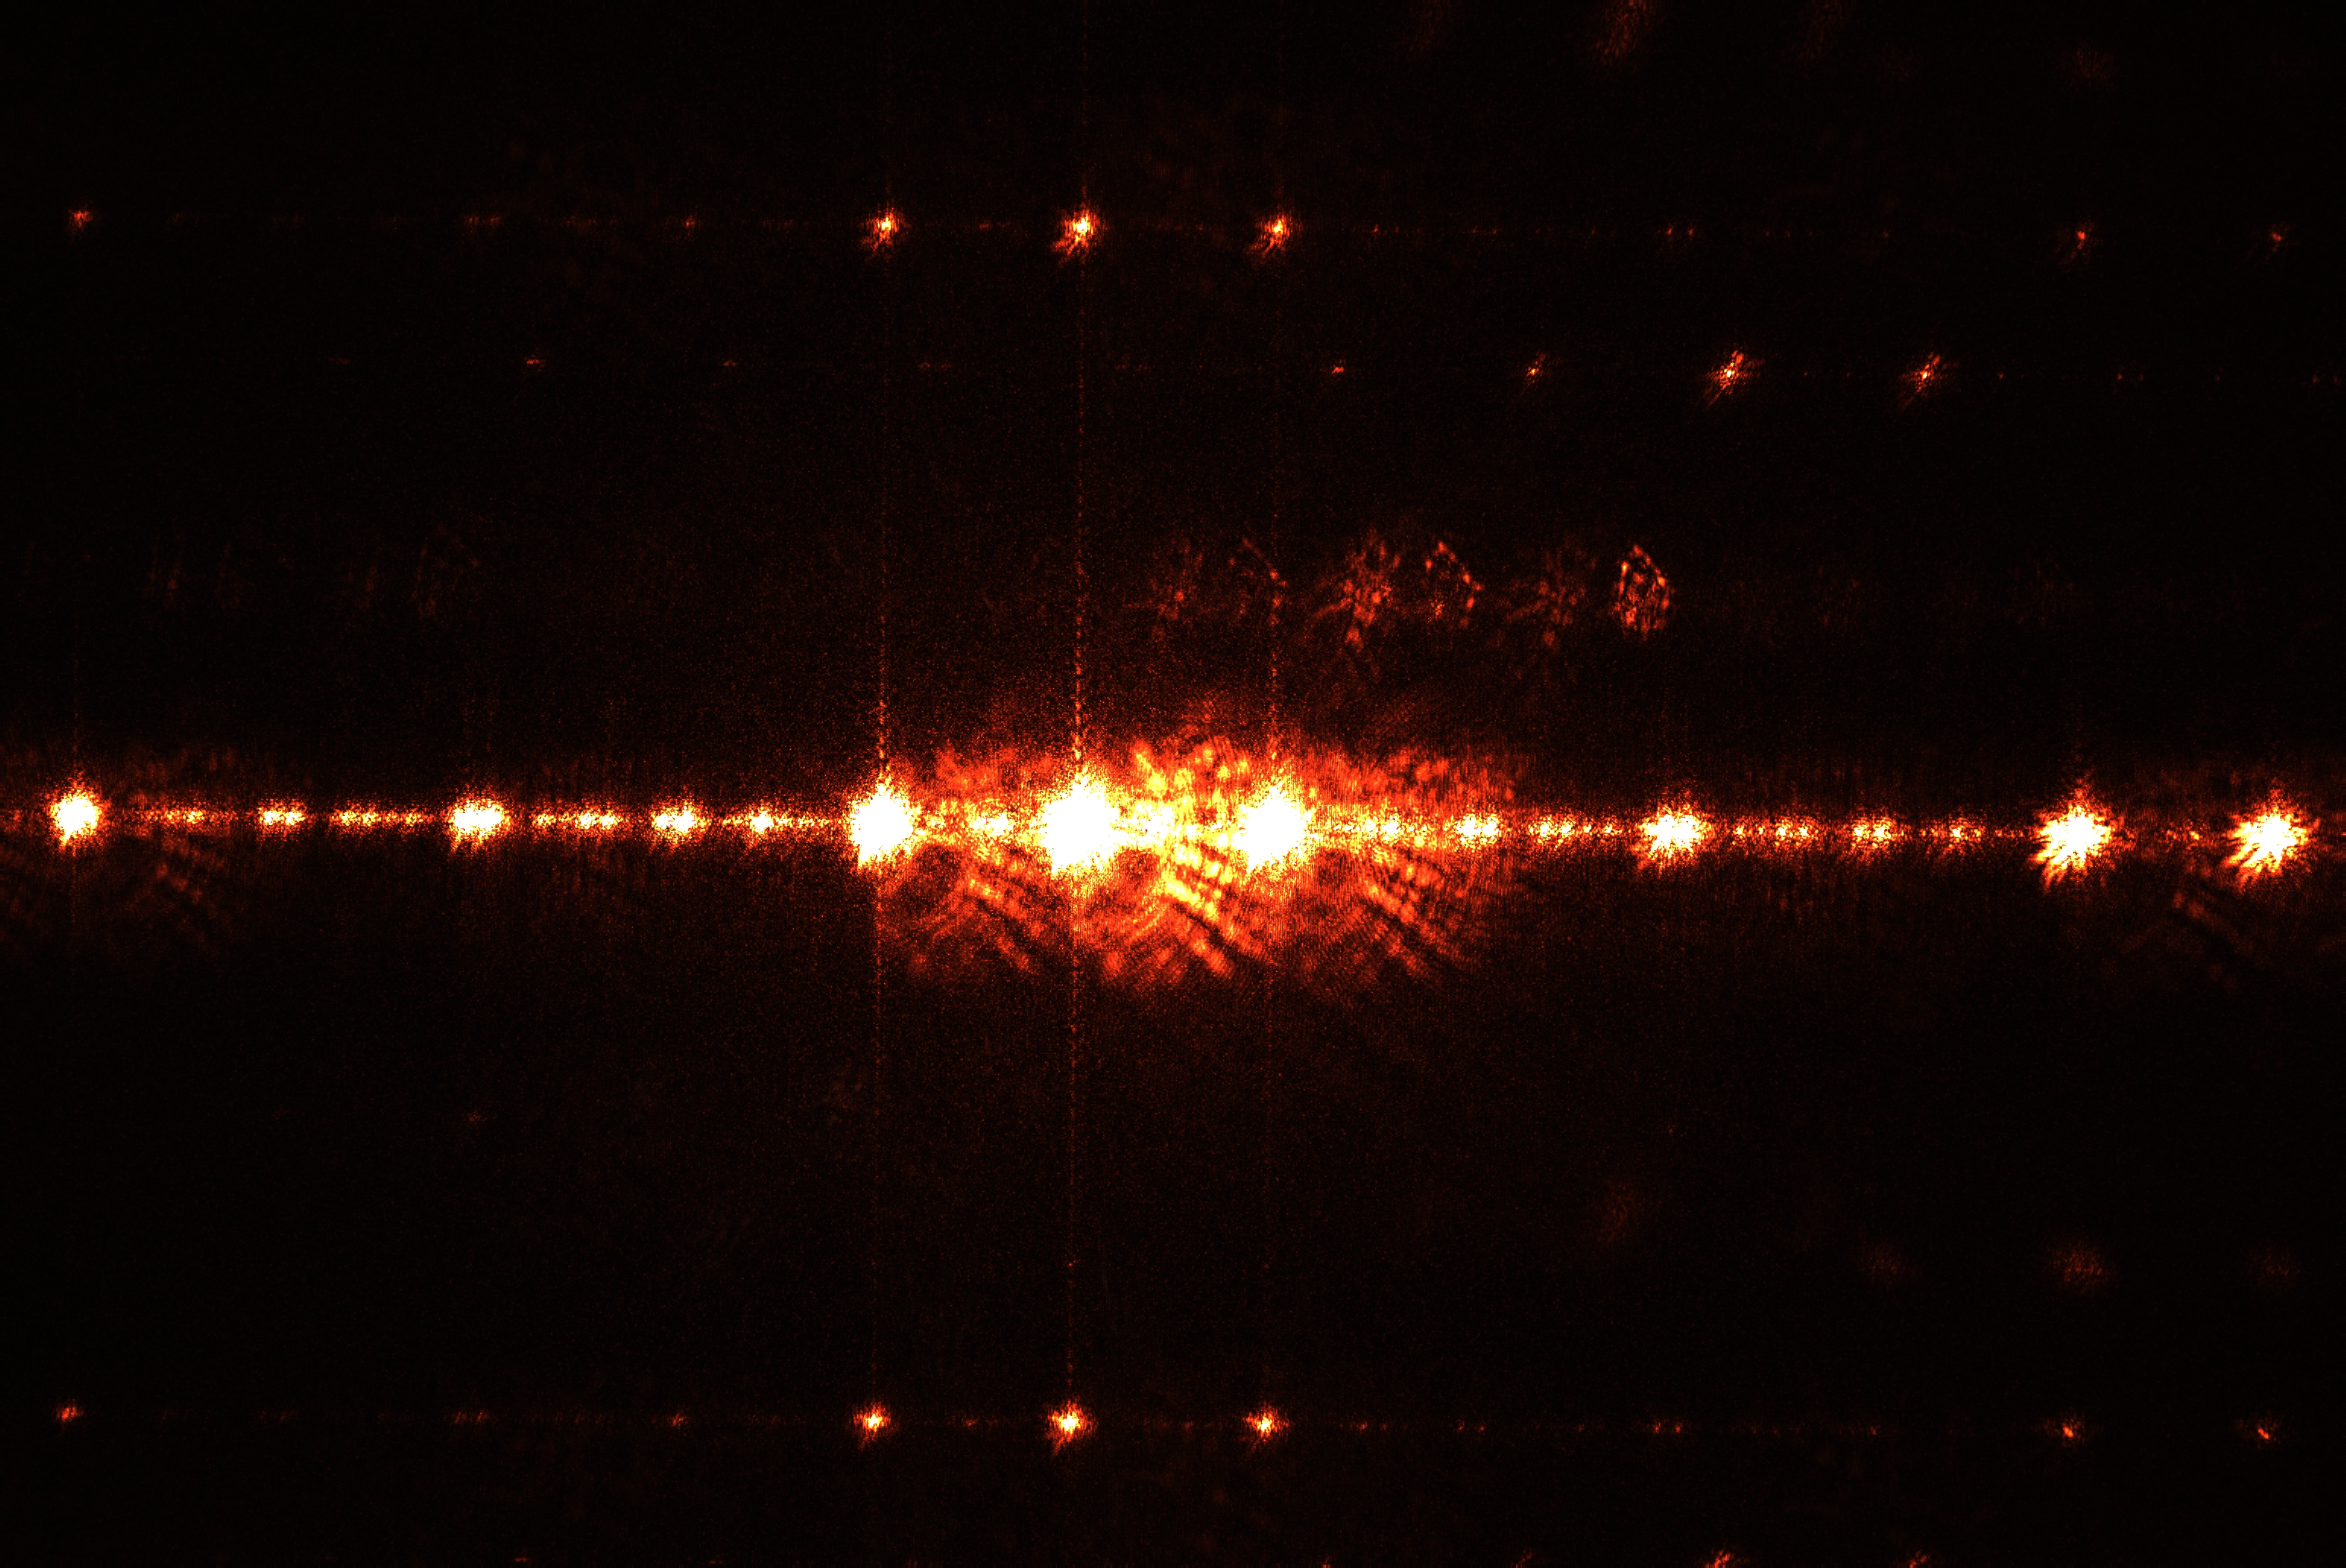
\includegraphics[width=0.3\textwidth]{C7.2/2/128T_p2.png}
	}%
	\caption{}
\end{figure}

频谱上的图案是一系列球对称于光轴的衍
射图案的组合,而处于光路中心的衍射图案
最亮,其余的衍射图案随远离光轴中心距离
增加而变暗。

同样在傅氏面$P_2$上放置可调狭缝,狭缝的刀口方向要与竖直方向的频谱平行。调节狭缝
的宽度,最后换成可变圆孔光阑,将x方向和y方向的频谱滤掉,观察并记录变化的情况,如图\ref{fig:ab2}.

\begin{figure}[H]
	\centering
	\subfloat[0级]{
	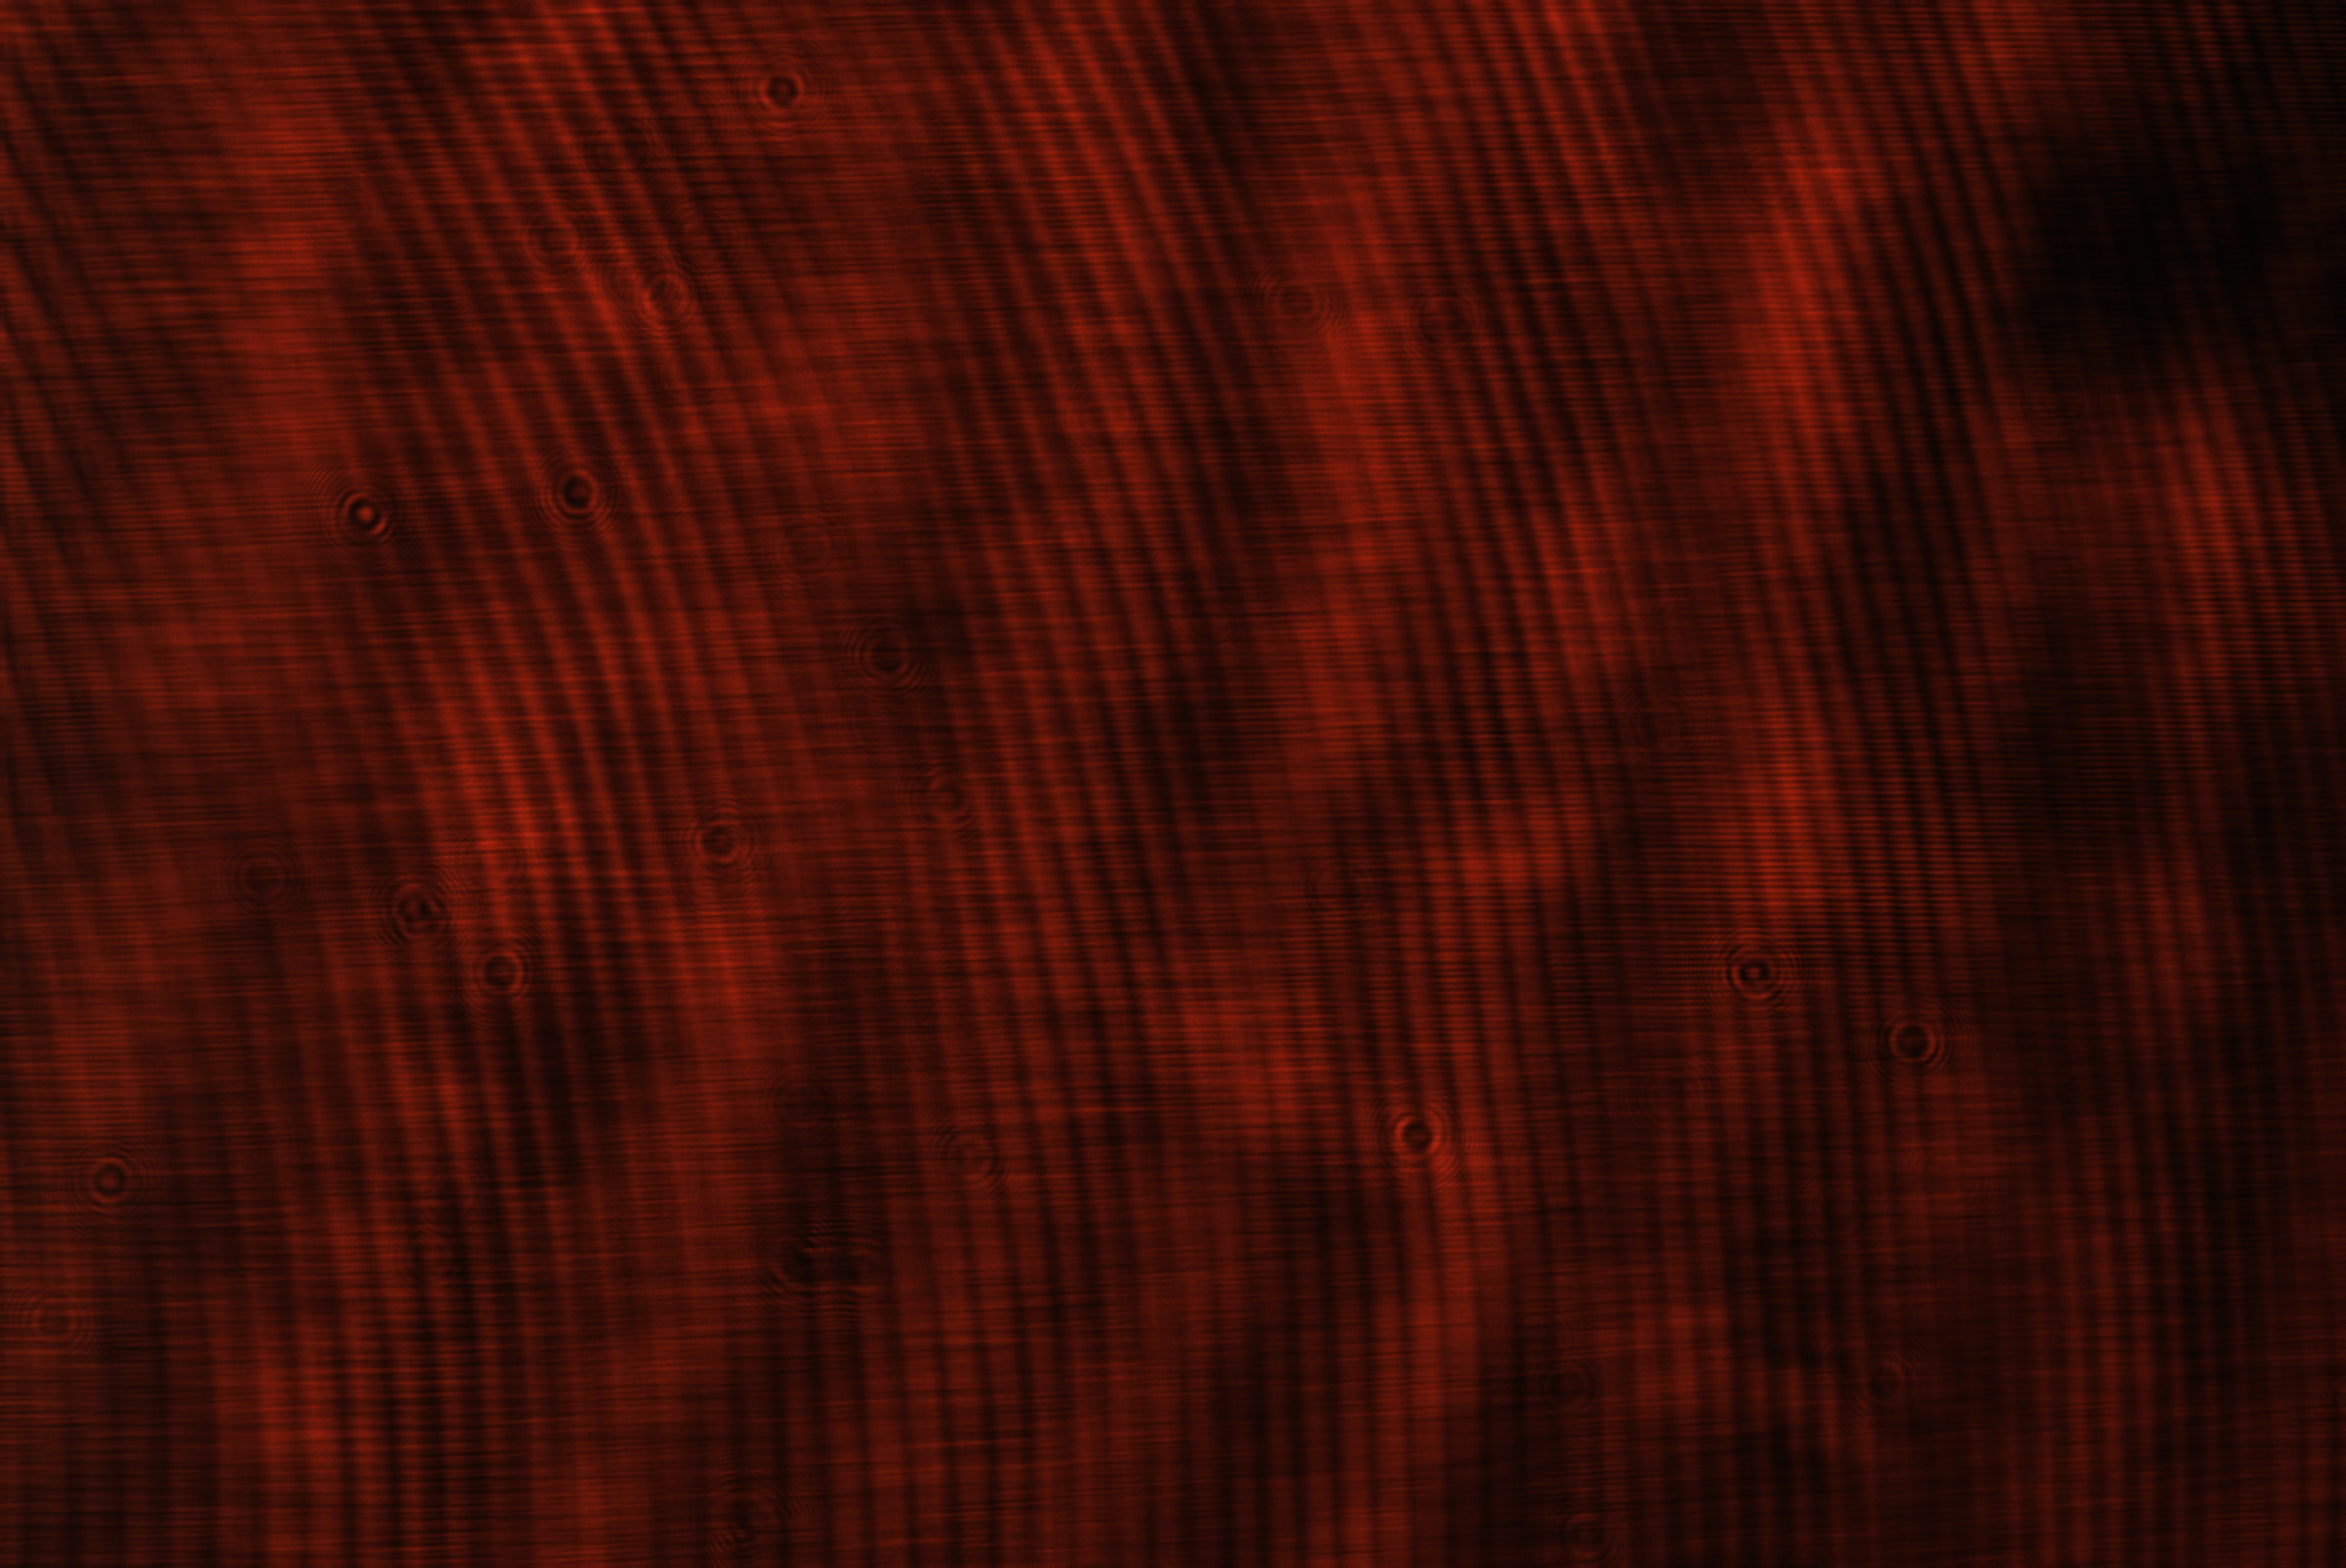
\includegraphics[width=0.3\textwidth]{C7.2/2/0.png}
	}%
	\subfloat[1级]{
	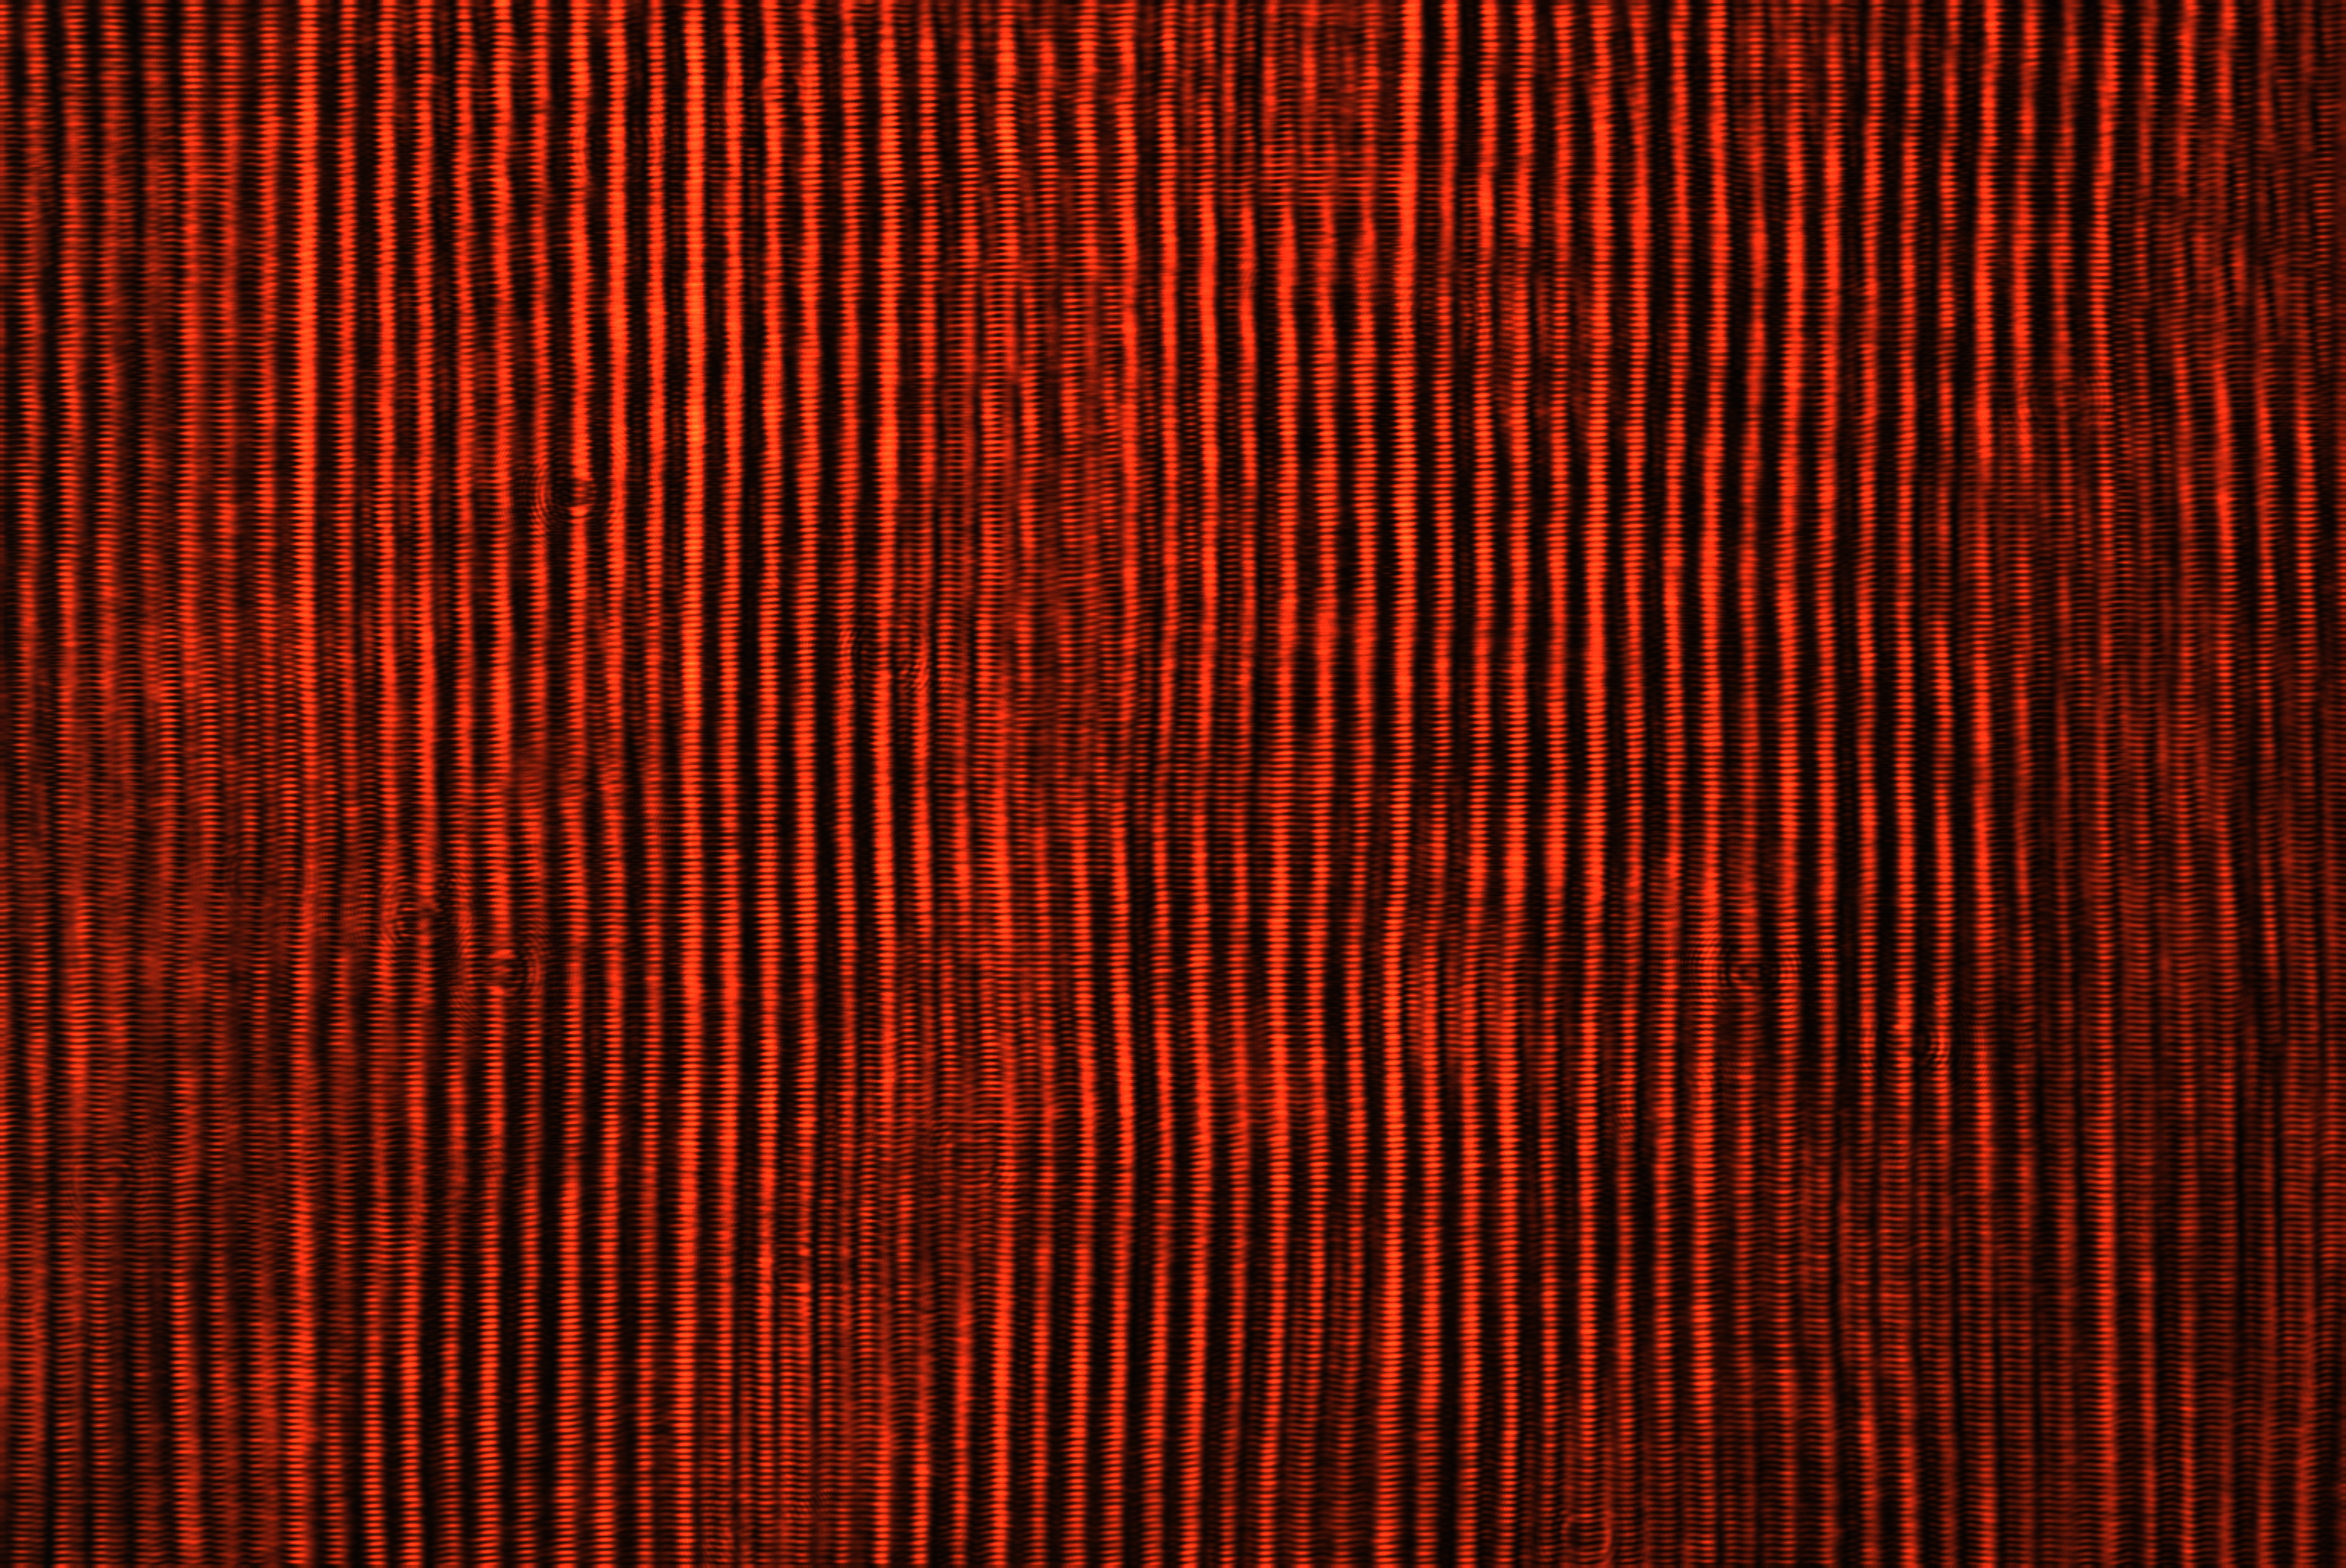
\includegraphics[width=0.3\textwidth]{C7.2/2/1.png}
	}%

	\subfloat[无狭缝]{
		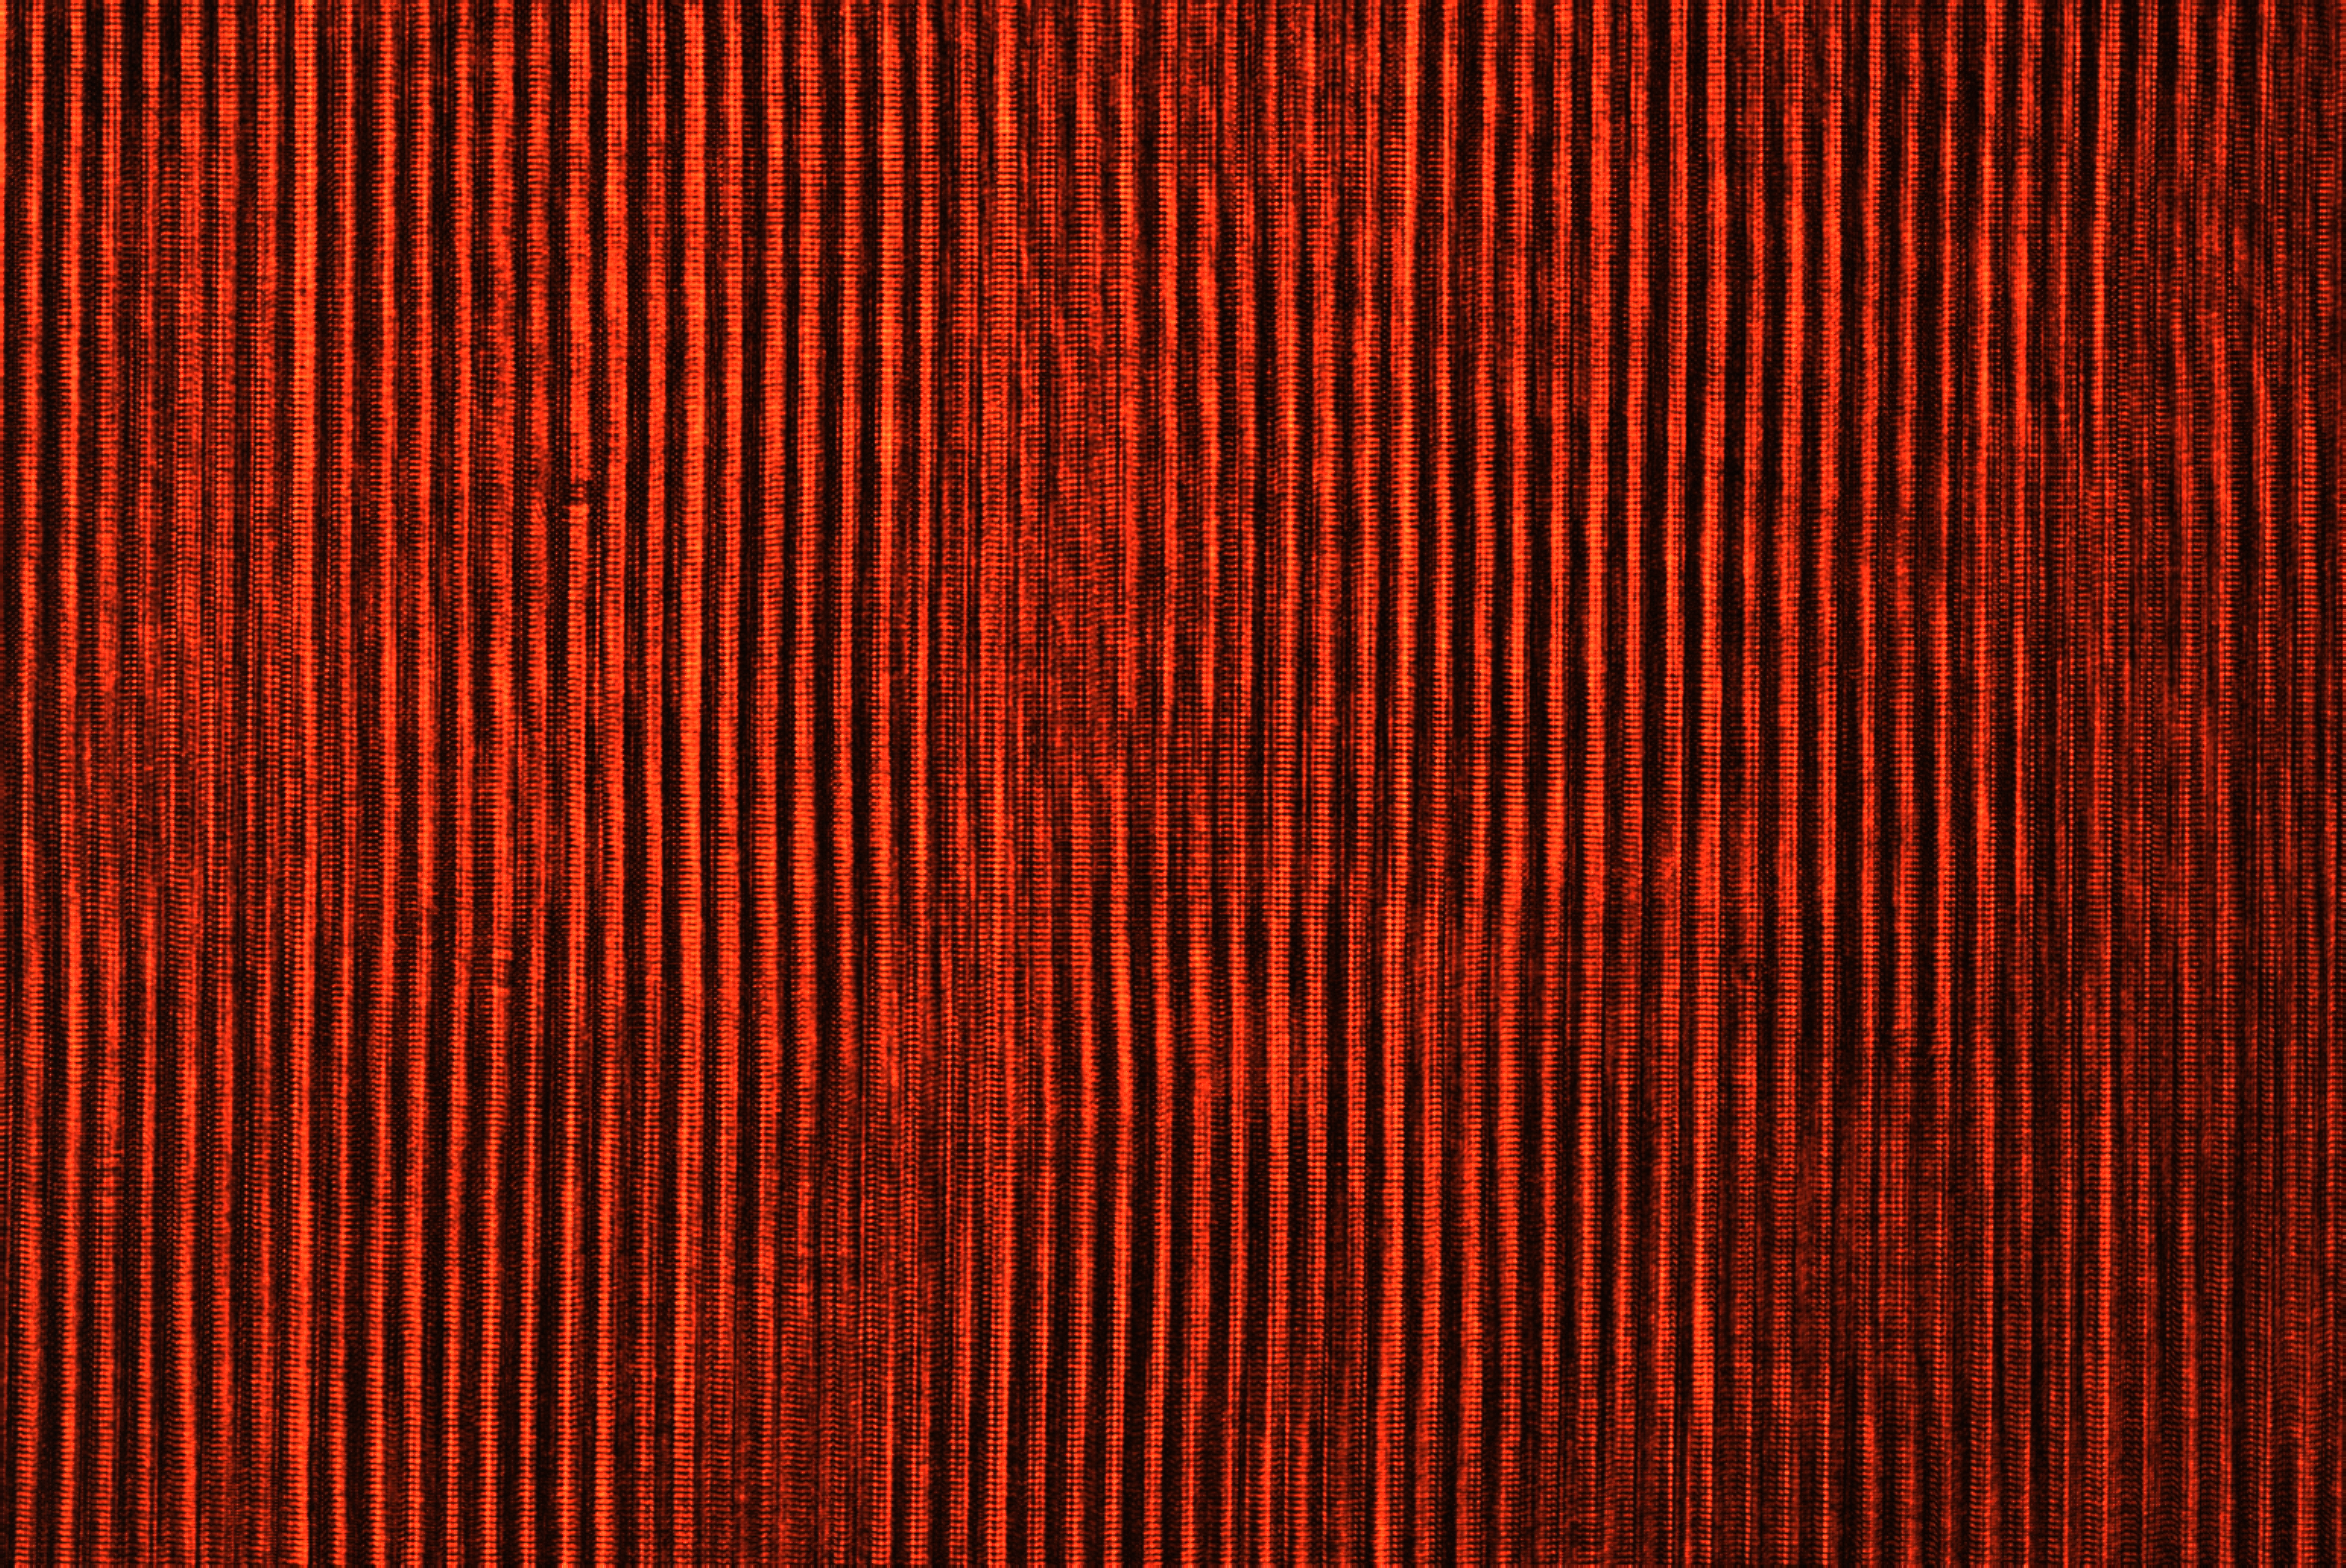
\includegraphics[width=0.3\textwidth]{C7.2/2/none.png}
	}%
	\subfloat[圆孔光阑]{
	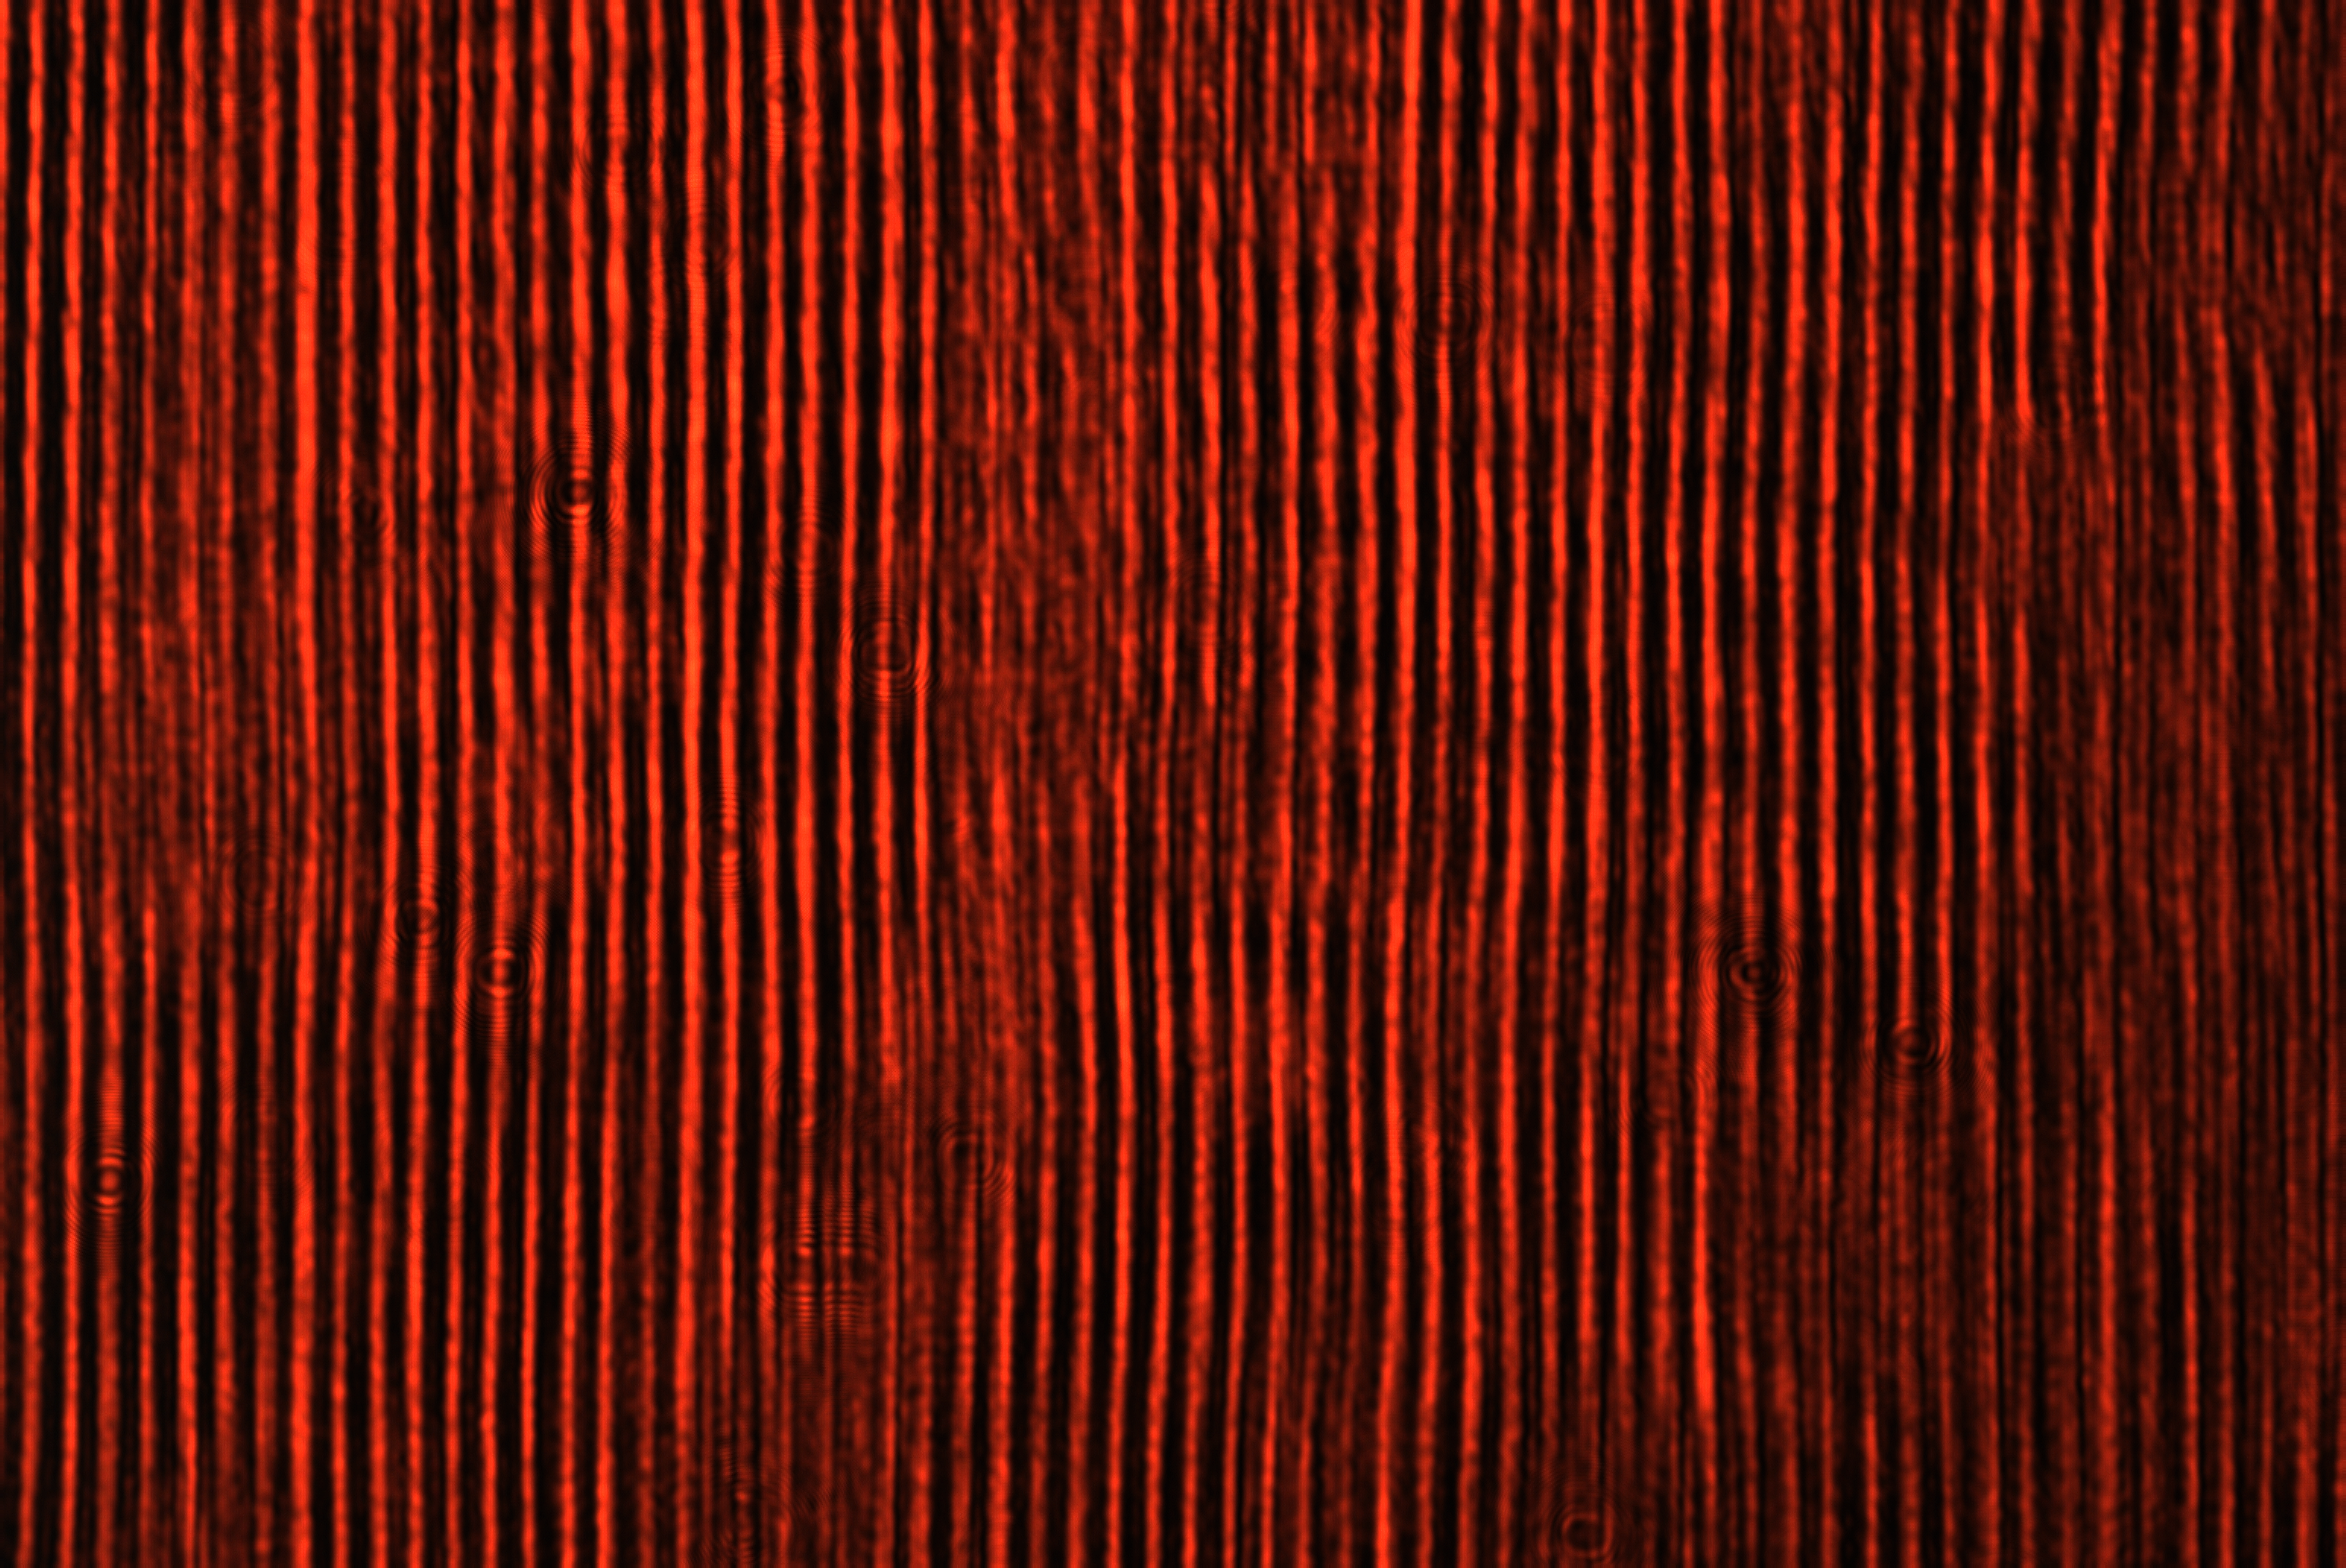
\includegraphics[width=0.3\textwidth]{C7.2/2/circ.png}
	}%
	\caption{空间光调制器光栅衍射成像}
	\label{fig:ab2}
\end{figure}

得到的结果与前述用实物光栅结果相
同结果从狭
缝很小到逐渐增大的过程中,像中条纹越来
越清晰,分辨率增加,细节得以慢慢呈现,
在狭缝很小但不为 0 时,像平面观察到竖直
的光栅变为水平。根据阿
贝成像原理,在频谱面上,光点的方向代表
该频率成分的方向,在狭缝很小时,只有竖
直方向上的频谱成分的以通过。由于空间光
调制器的表面实际是网格化的,所以加载的
光栅中透过光的部分实际是点阵,也可以理
解为一个二维正交光栅。狭缝很小使得只有
二维光栅的纵向结构的信息通过,而这些纵
向的频谱在像平面上合成了横向的光栅图
像,所以在像的图案出现相当密集的水平的
条纹。

将可调狭缝换为圆孔光阑,挡住除中
心外的 x、y 方向上的其余多组衍射图,可知
图像的细节会减小,这是
因为高频信息被逐渐过滤掉,具体原理如前
所述。

\subsubsection{低通滤波和高通滤波}
低通滤波器可让接近零级的低频成分通过而除去高频成分,可用于滤除高频噪声(例如消除照
片中的网纹或减轻颗粒影响)。高通滤波器能限制连续色调而强化锐边,有助于细节观察。

将空间光调制器的图案换成网格光图案在像平面P上观察像的构成。图的像素可用周期性空间函数表示,其频
谱是有规律排列的分立点阵;而图的外形是非周期性的低频信号,其频谱是连续的。
分别将低通滤波器和高通滤波器,放在傅氏面上,让低级光点通过,观察
像的构成,如图\ref{fig:hl}.
\begin{figure}[H]
	\centering
	\subfloat[网格光图案]{
	\includegraphics[width=0.3\textwidth]{C7.2/3/网格“光” - 副本.png}
	}%
	\subfloat[像平面P上像]{
	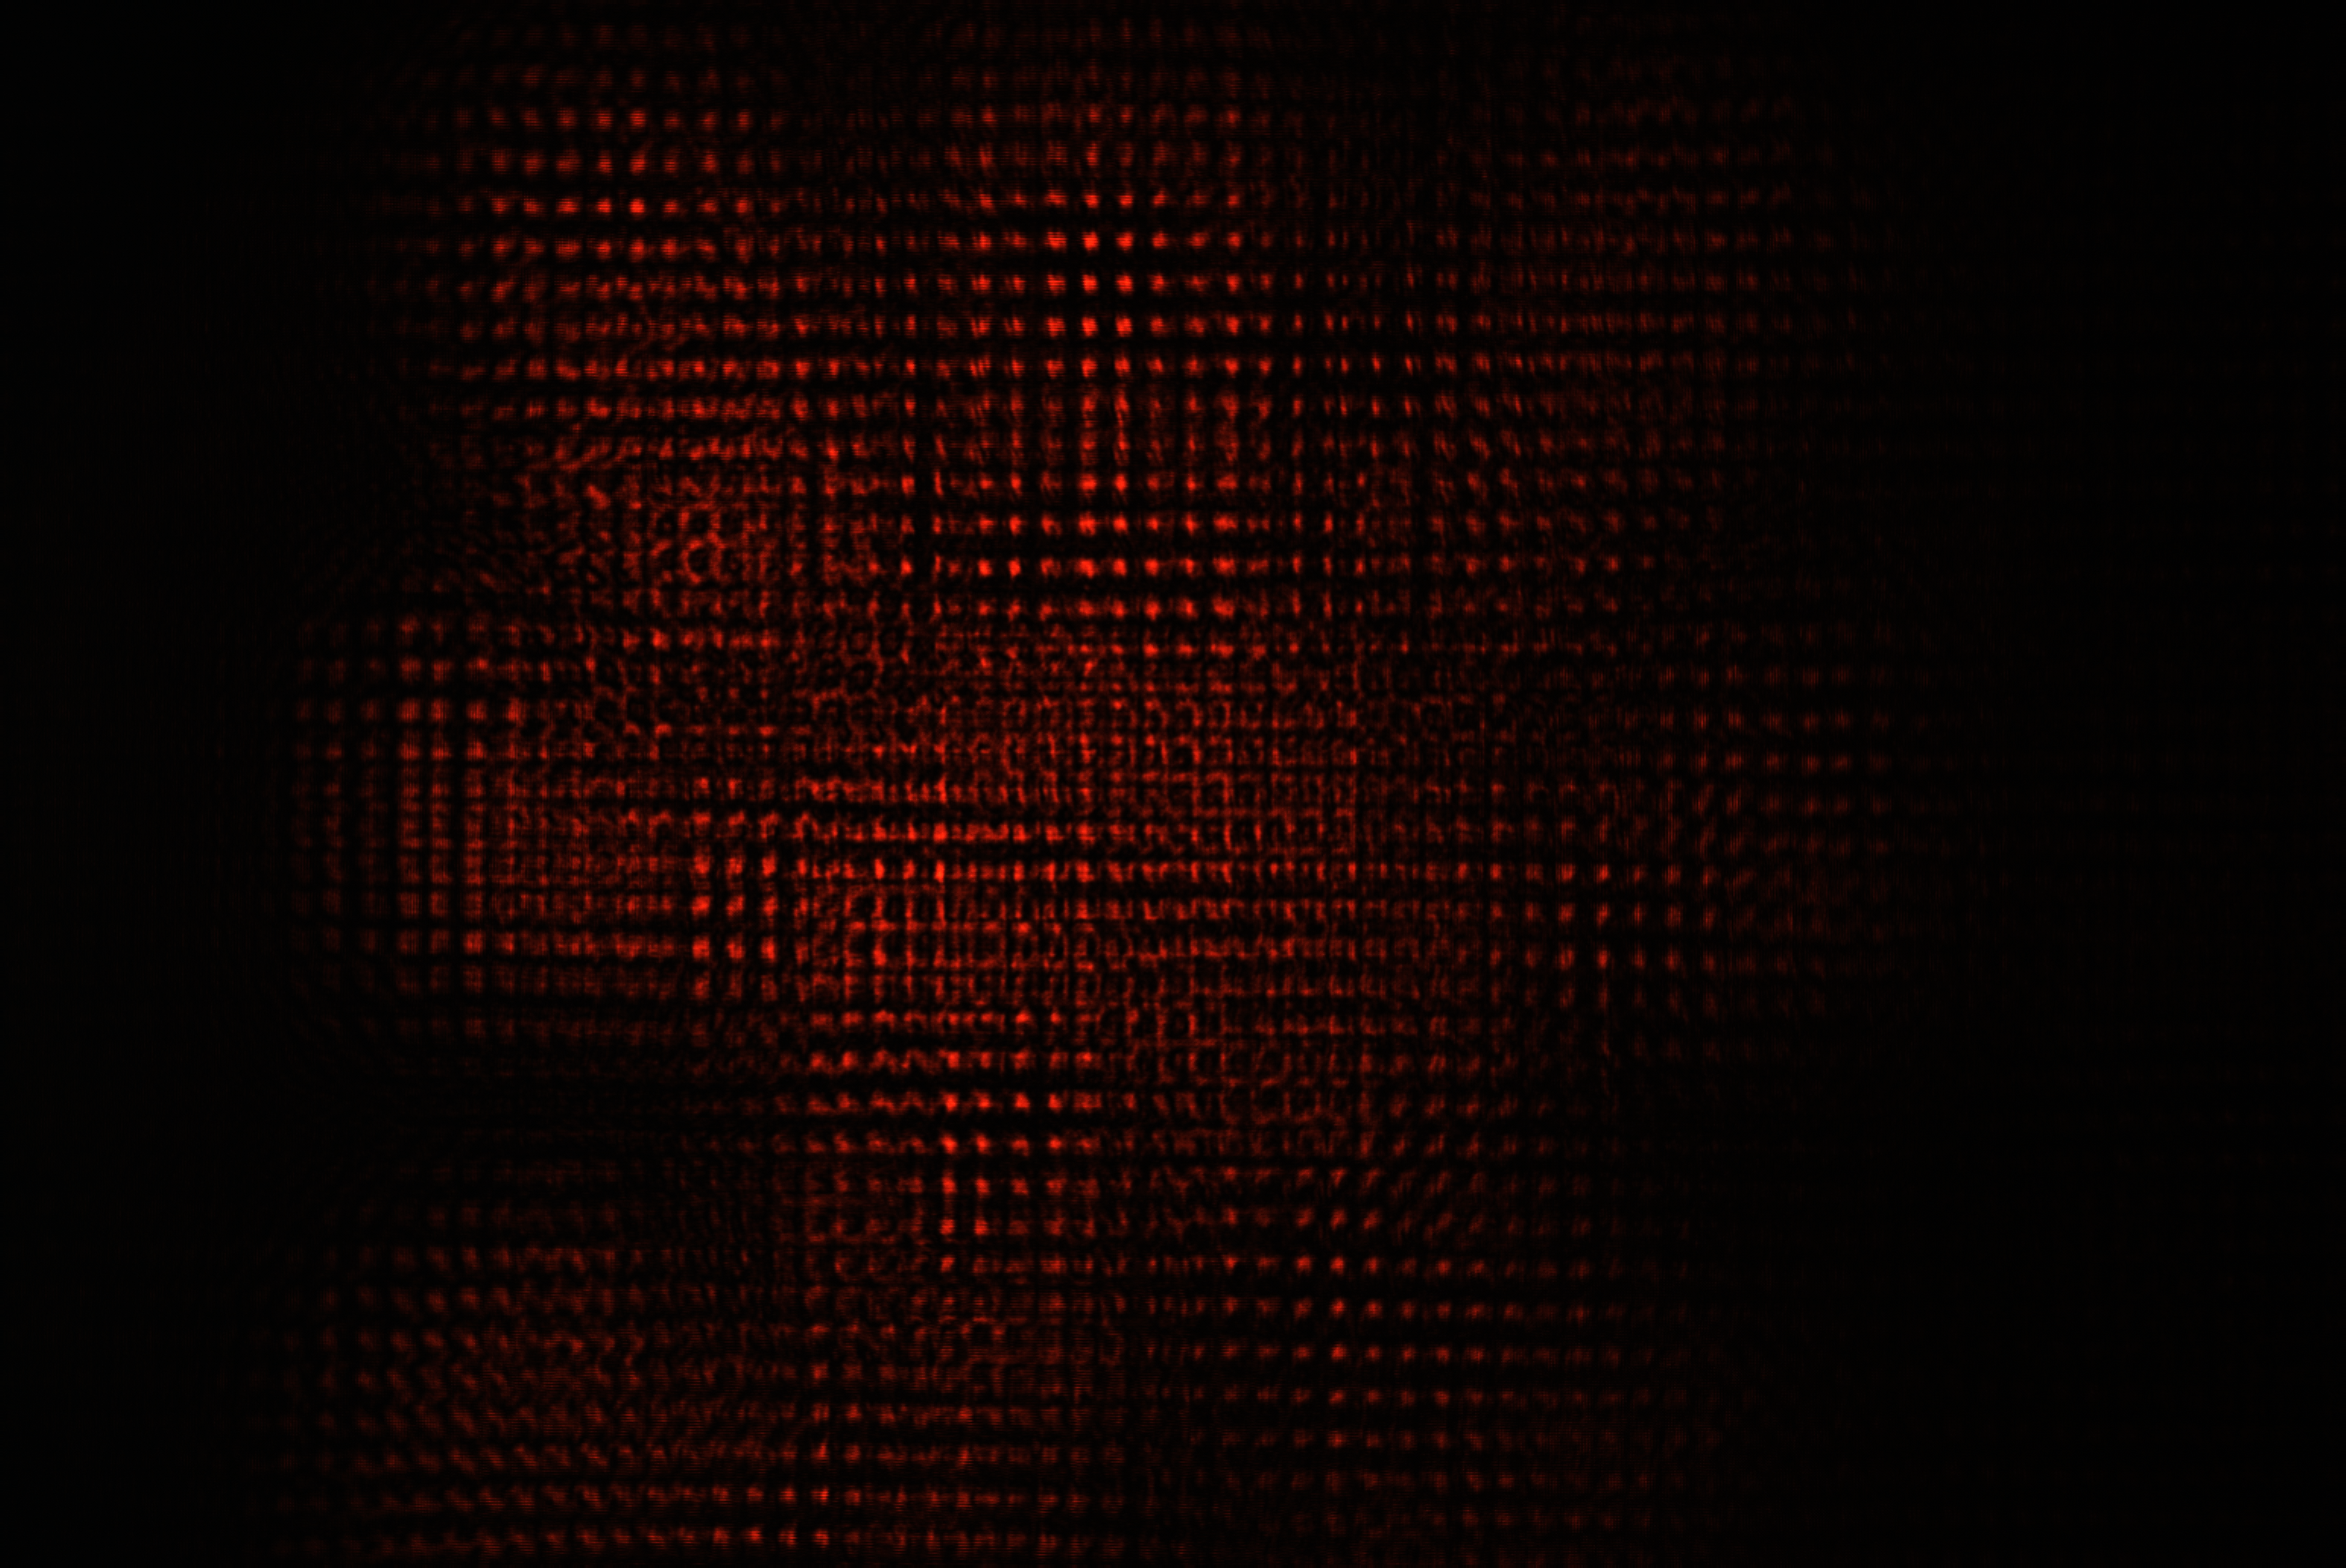
\includegraphics[width=0.3\textwidth]{C7.2/3/guang.png}
	}%

	\subfloat[高通滤波]{
		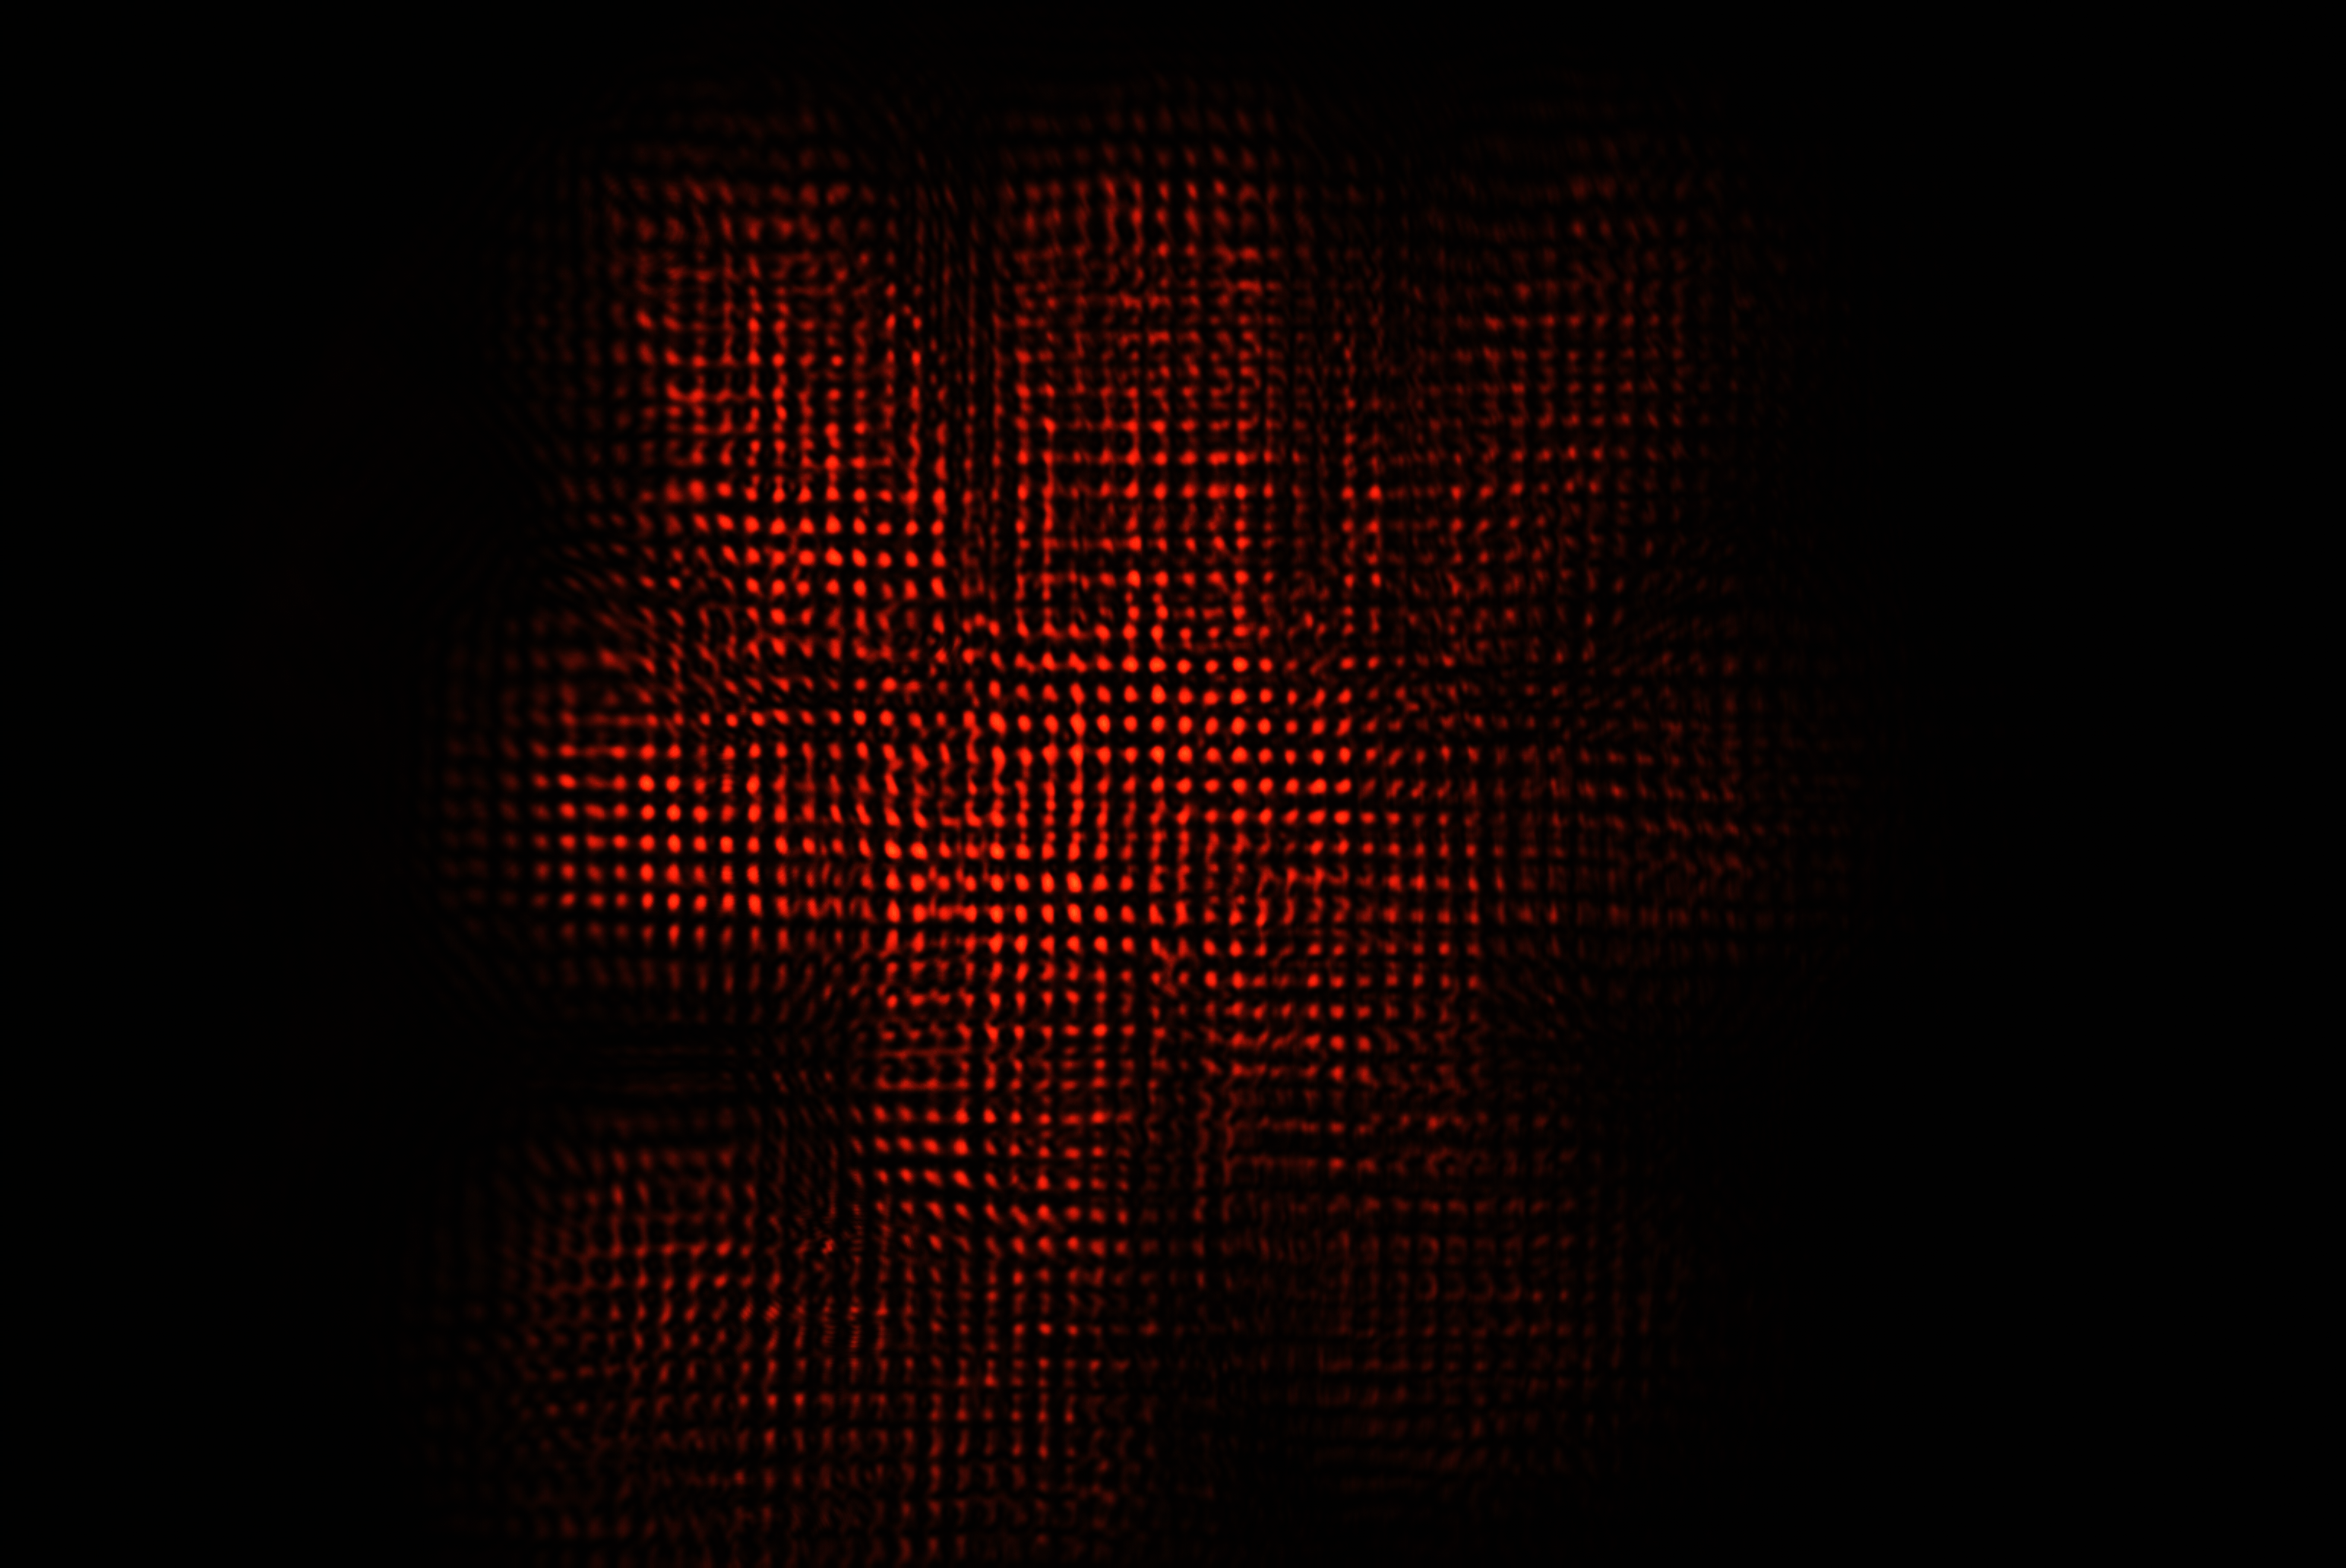
\includegraphics[width=0.3\textwidth]{C7.2/3/high.png}
	}%
	\subfloat[低通滤波]{
	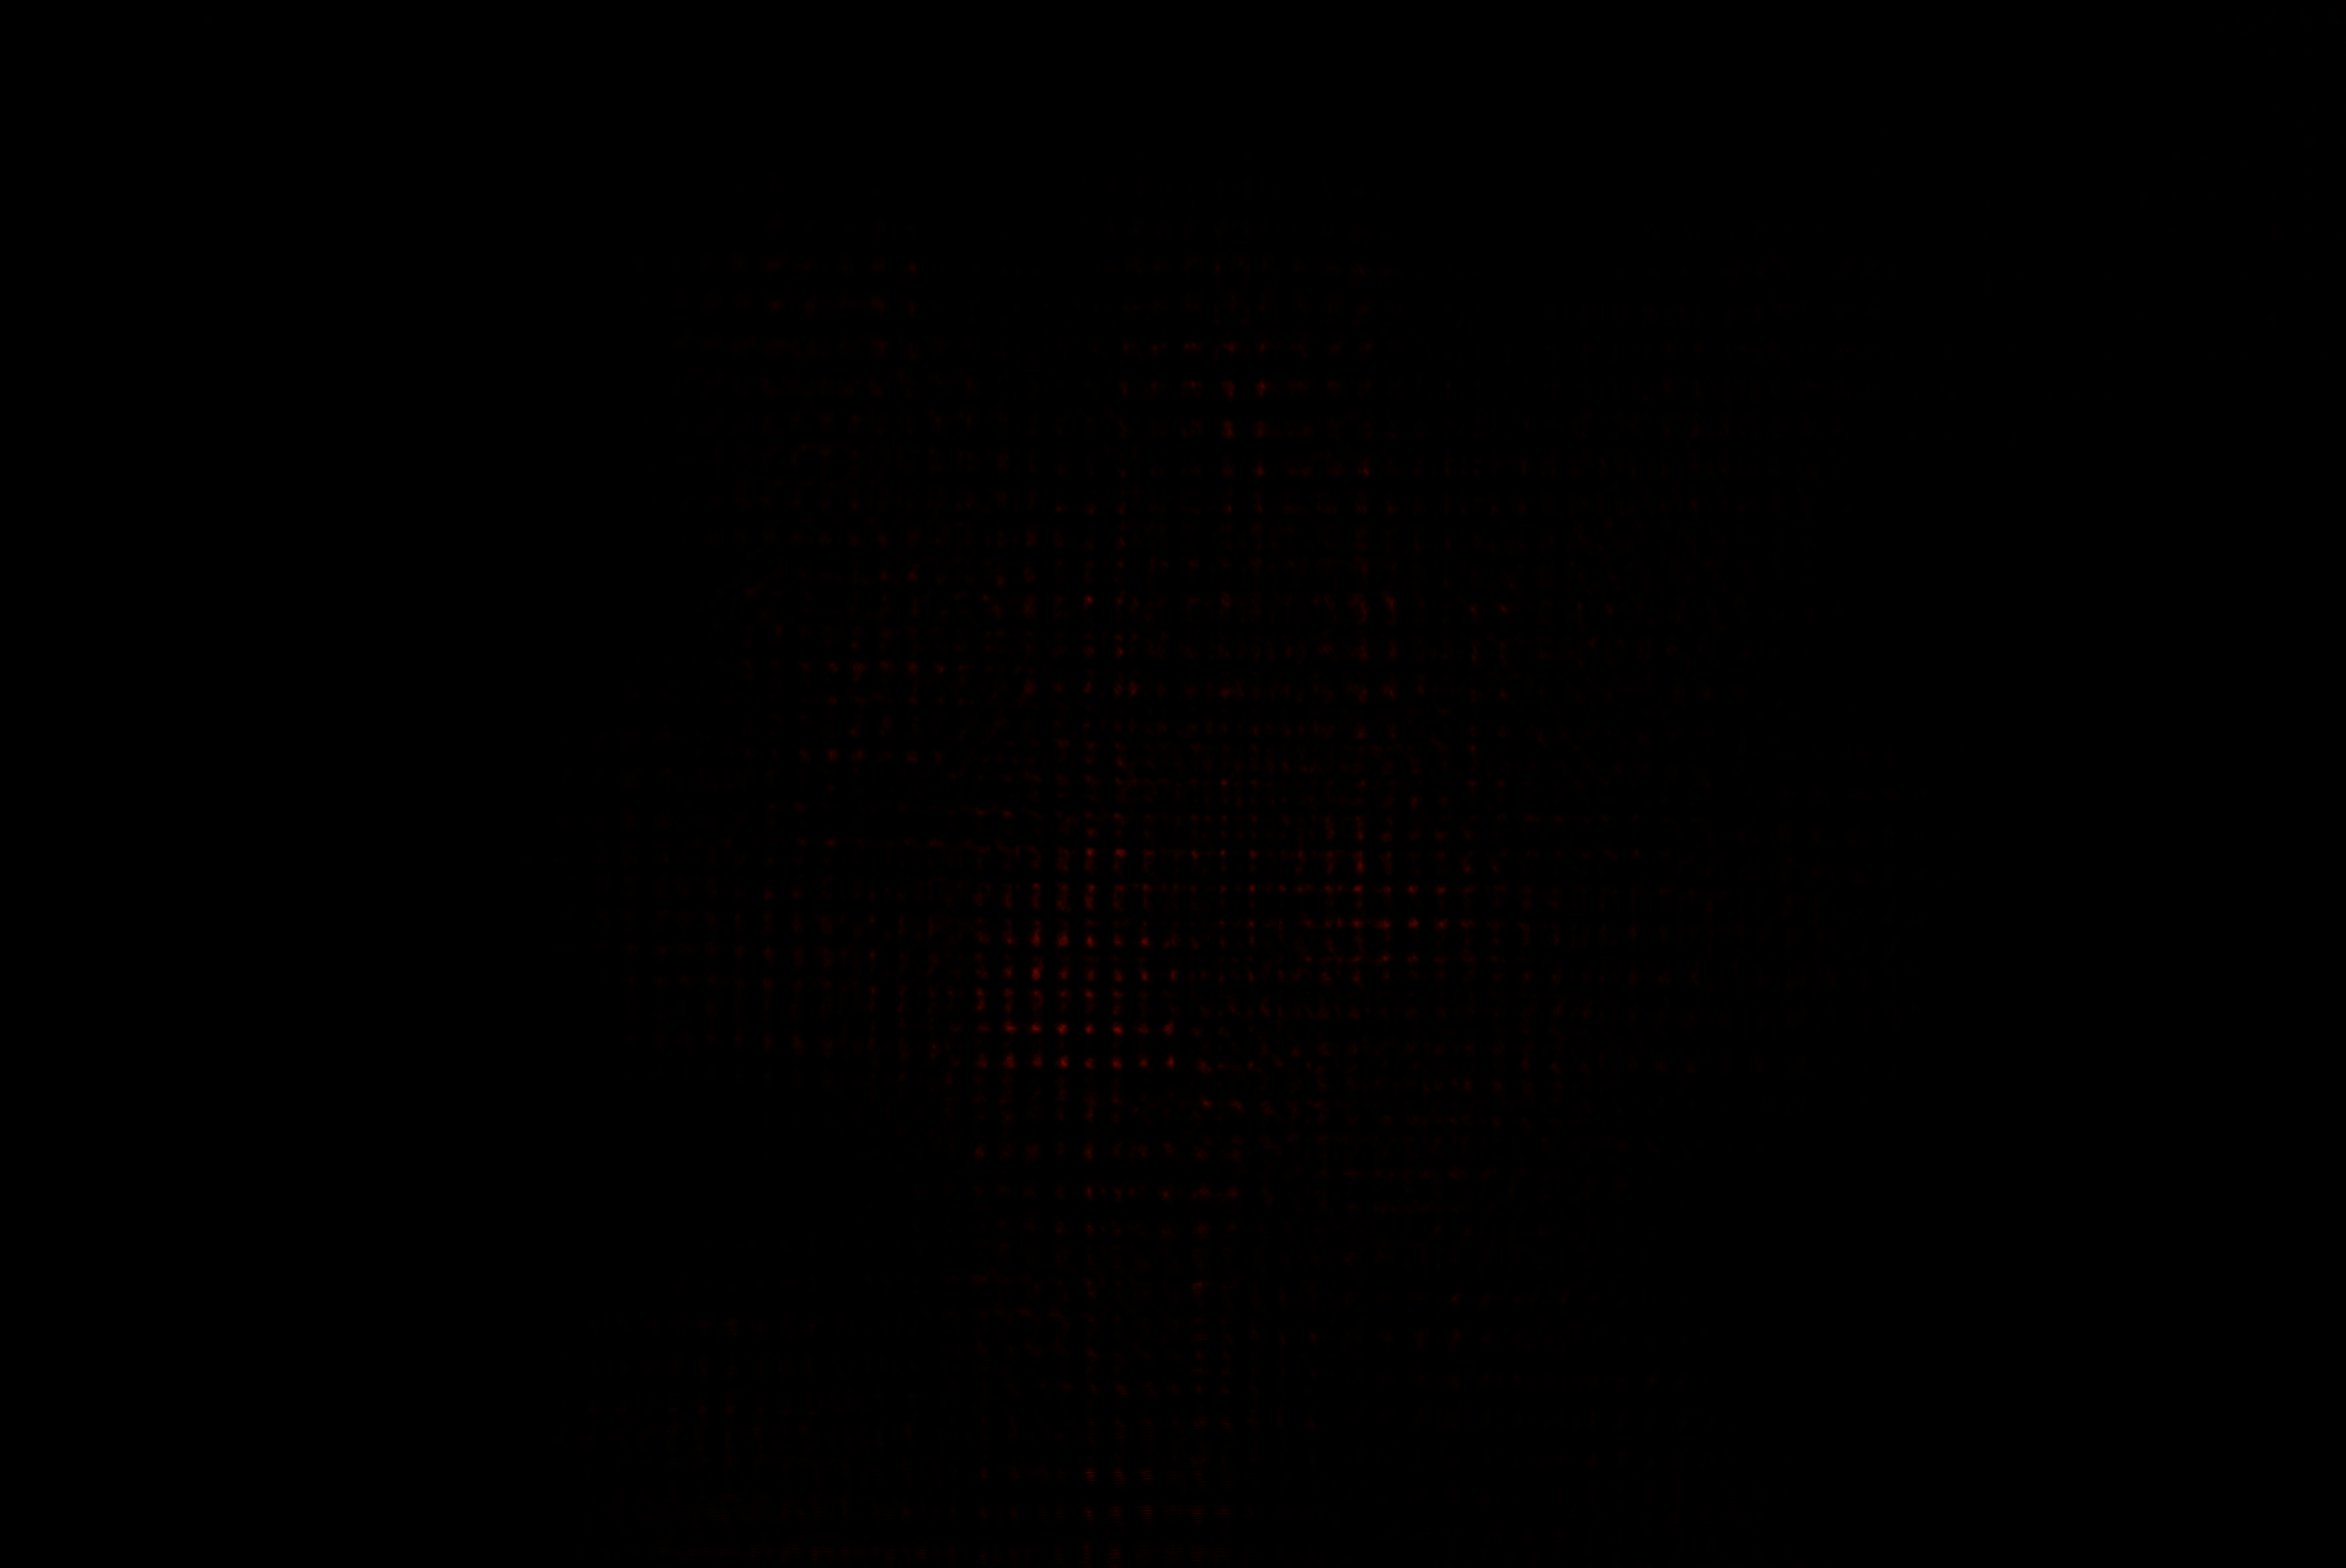
\includegraphics[width=0.3\textwidth]{C7.2/3/low.png}
	}%
	\caption{频率滤波成像}
	\label{fig:hl}
\end{figure}

对比通过低通滤波的像和原像,最明显
的区别是“光”字内部的网格被过滤了。这
是因为照片中的网纹,类似于光栅图案,其
在傅氏面上的频谱样式是分离的谱点,除了
离光轴很近的低频信息,其高频信息对成像
也很重要;而“光”字的笔画粗,具有的是
低频信息为主,所以通过低频滤波器之后,
只有笔画的频谱信息和网格的低频信息被
保留,网格的高频信息被过滤掉,而保留下
来的网格的低频信息是一个基本均匀的光
照,所以最终的图像是消去了网纹的光字。
而通过高通滤波器的像与原像相比,区
别在于前者更容易观察细节,锐化度更高。
这是因为高频代表的细节被保留,低频对应
的像被削弱,相同的低频成分被滤去,
所以提高了对比度。

\subsubsection{方向滤波}
在空间光调制器上加载二维正交光栅,可在傅氏面上观察到衍射光的二维点阵,即
正交光栅的傅里叶空间频谱,而在像平面 P 上可看到正交光栅的像,如图\ref{fig:dir_raw}.

\begin{figure}[H]
	\centering
	\subfloat[128T$\times $96T 二维光栅]{
	\includegraphics[width=0.3\textwidth]{C7.2/4/128T乘96T二维光栅.png}
	}%
	\subfloat[正交光栅的傅里叶空间频谱]{
	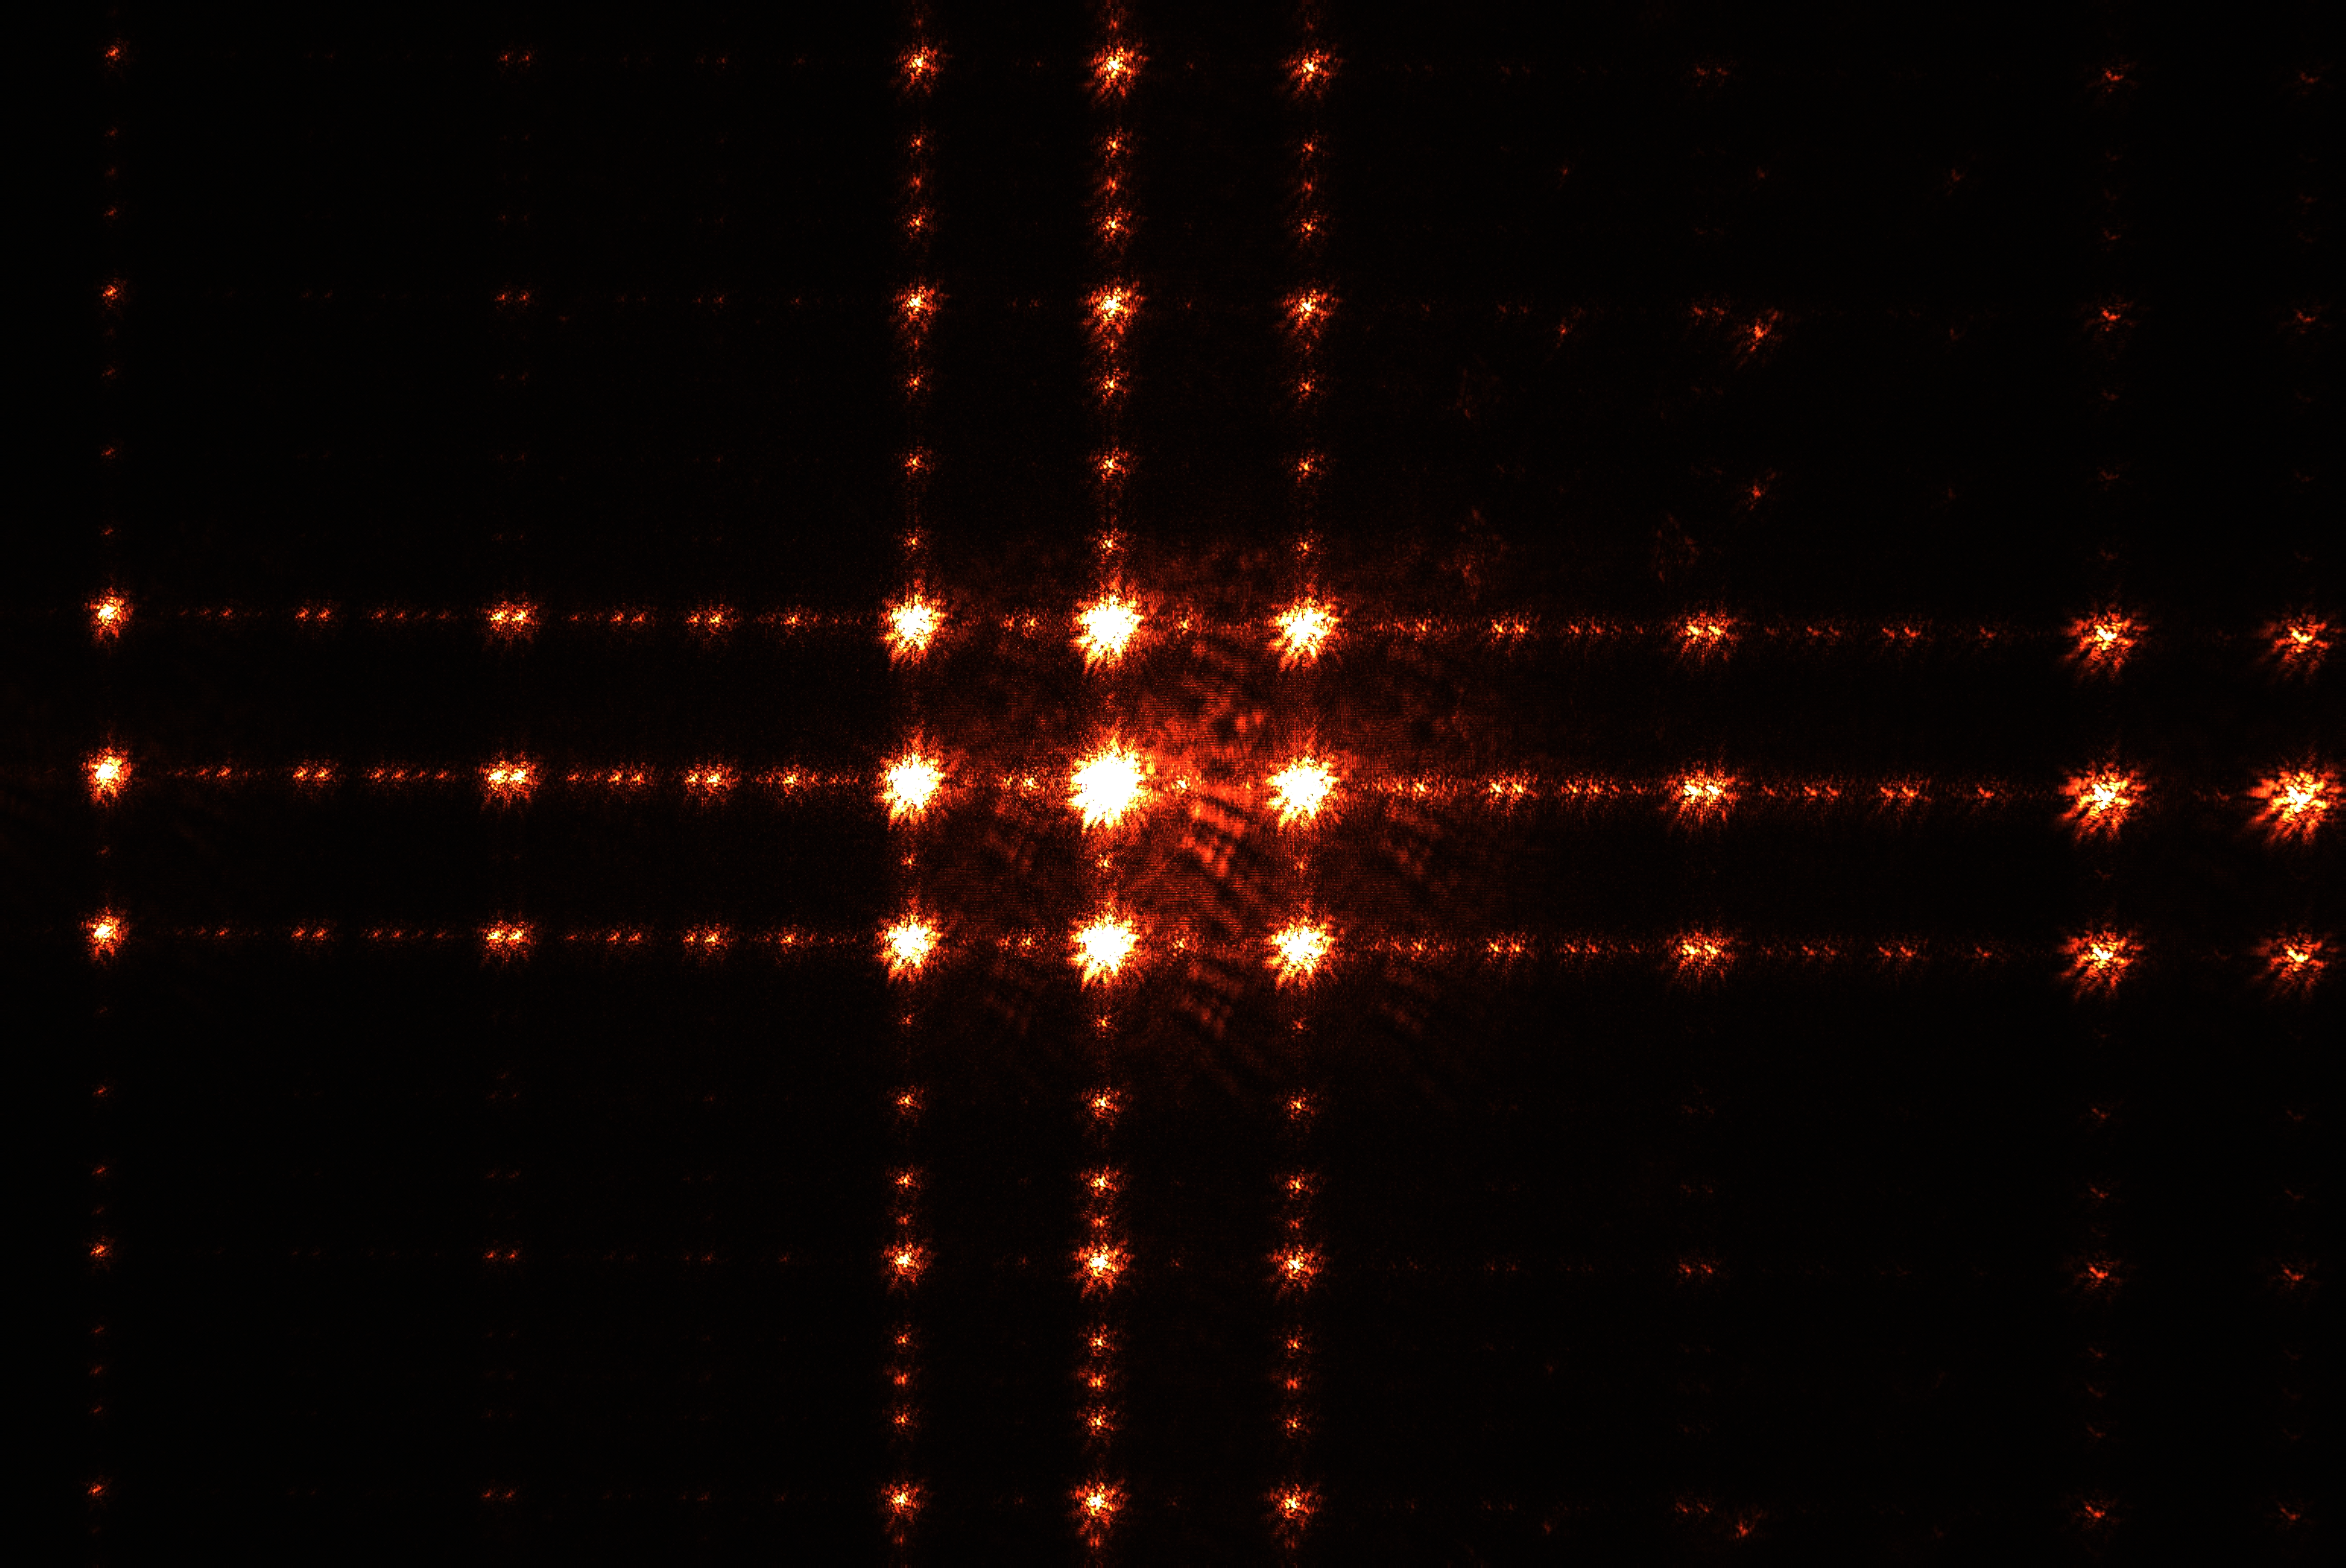
\includegraphics[width=0.3\textwidth]{C7.2/4/128x96_p2.png}
	}%
	\caption{}
	\label{fig:dir_raw}
\end{figure}

将可调狭缝放在傅氏面上,狭缝处于竖直方向。调节狭缝的大小,
使只有中间一列衍射光斑通过狭缝。将狭缝绕光轴旋转,分别
置于水平、沿45°、垂直和沿135°,成像如图\ref{fig:dir}.
\begin{figure}[H]
	\centering
	\subfloat[狭缝水平]{
	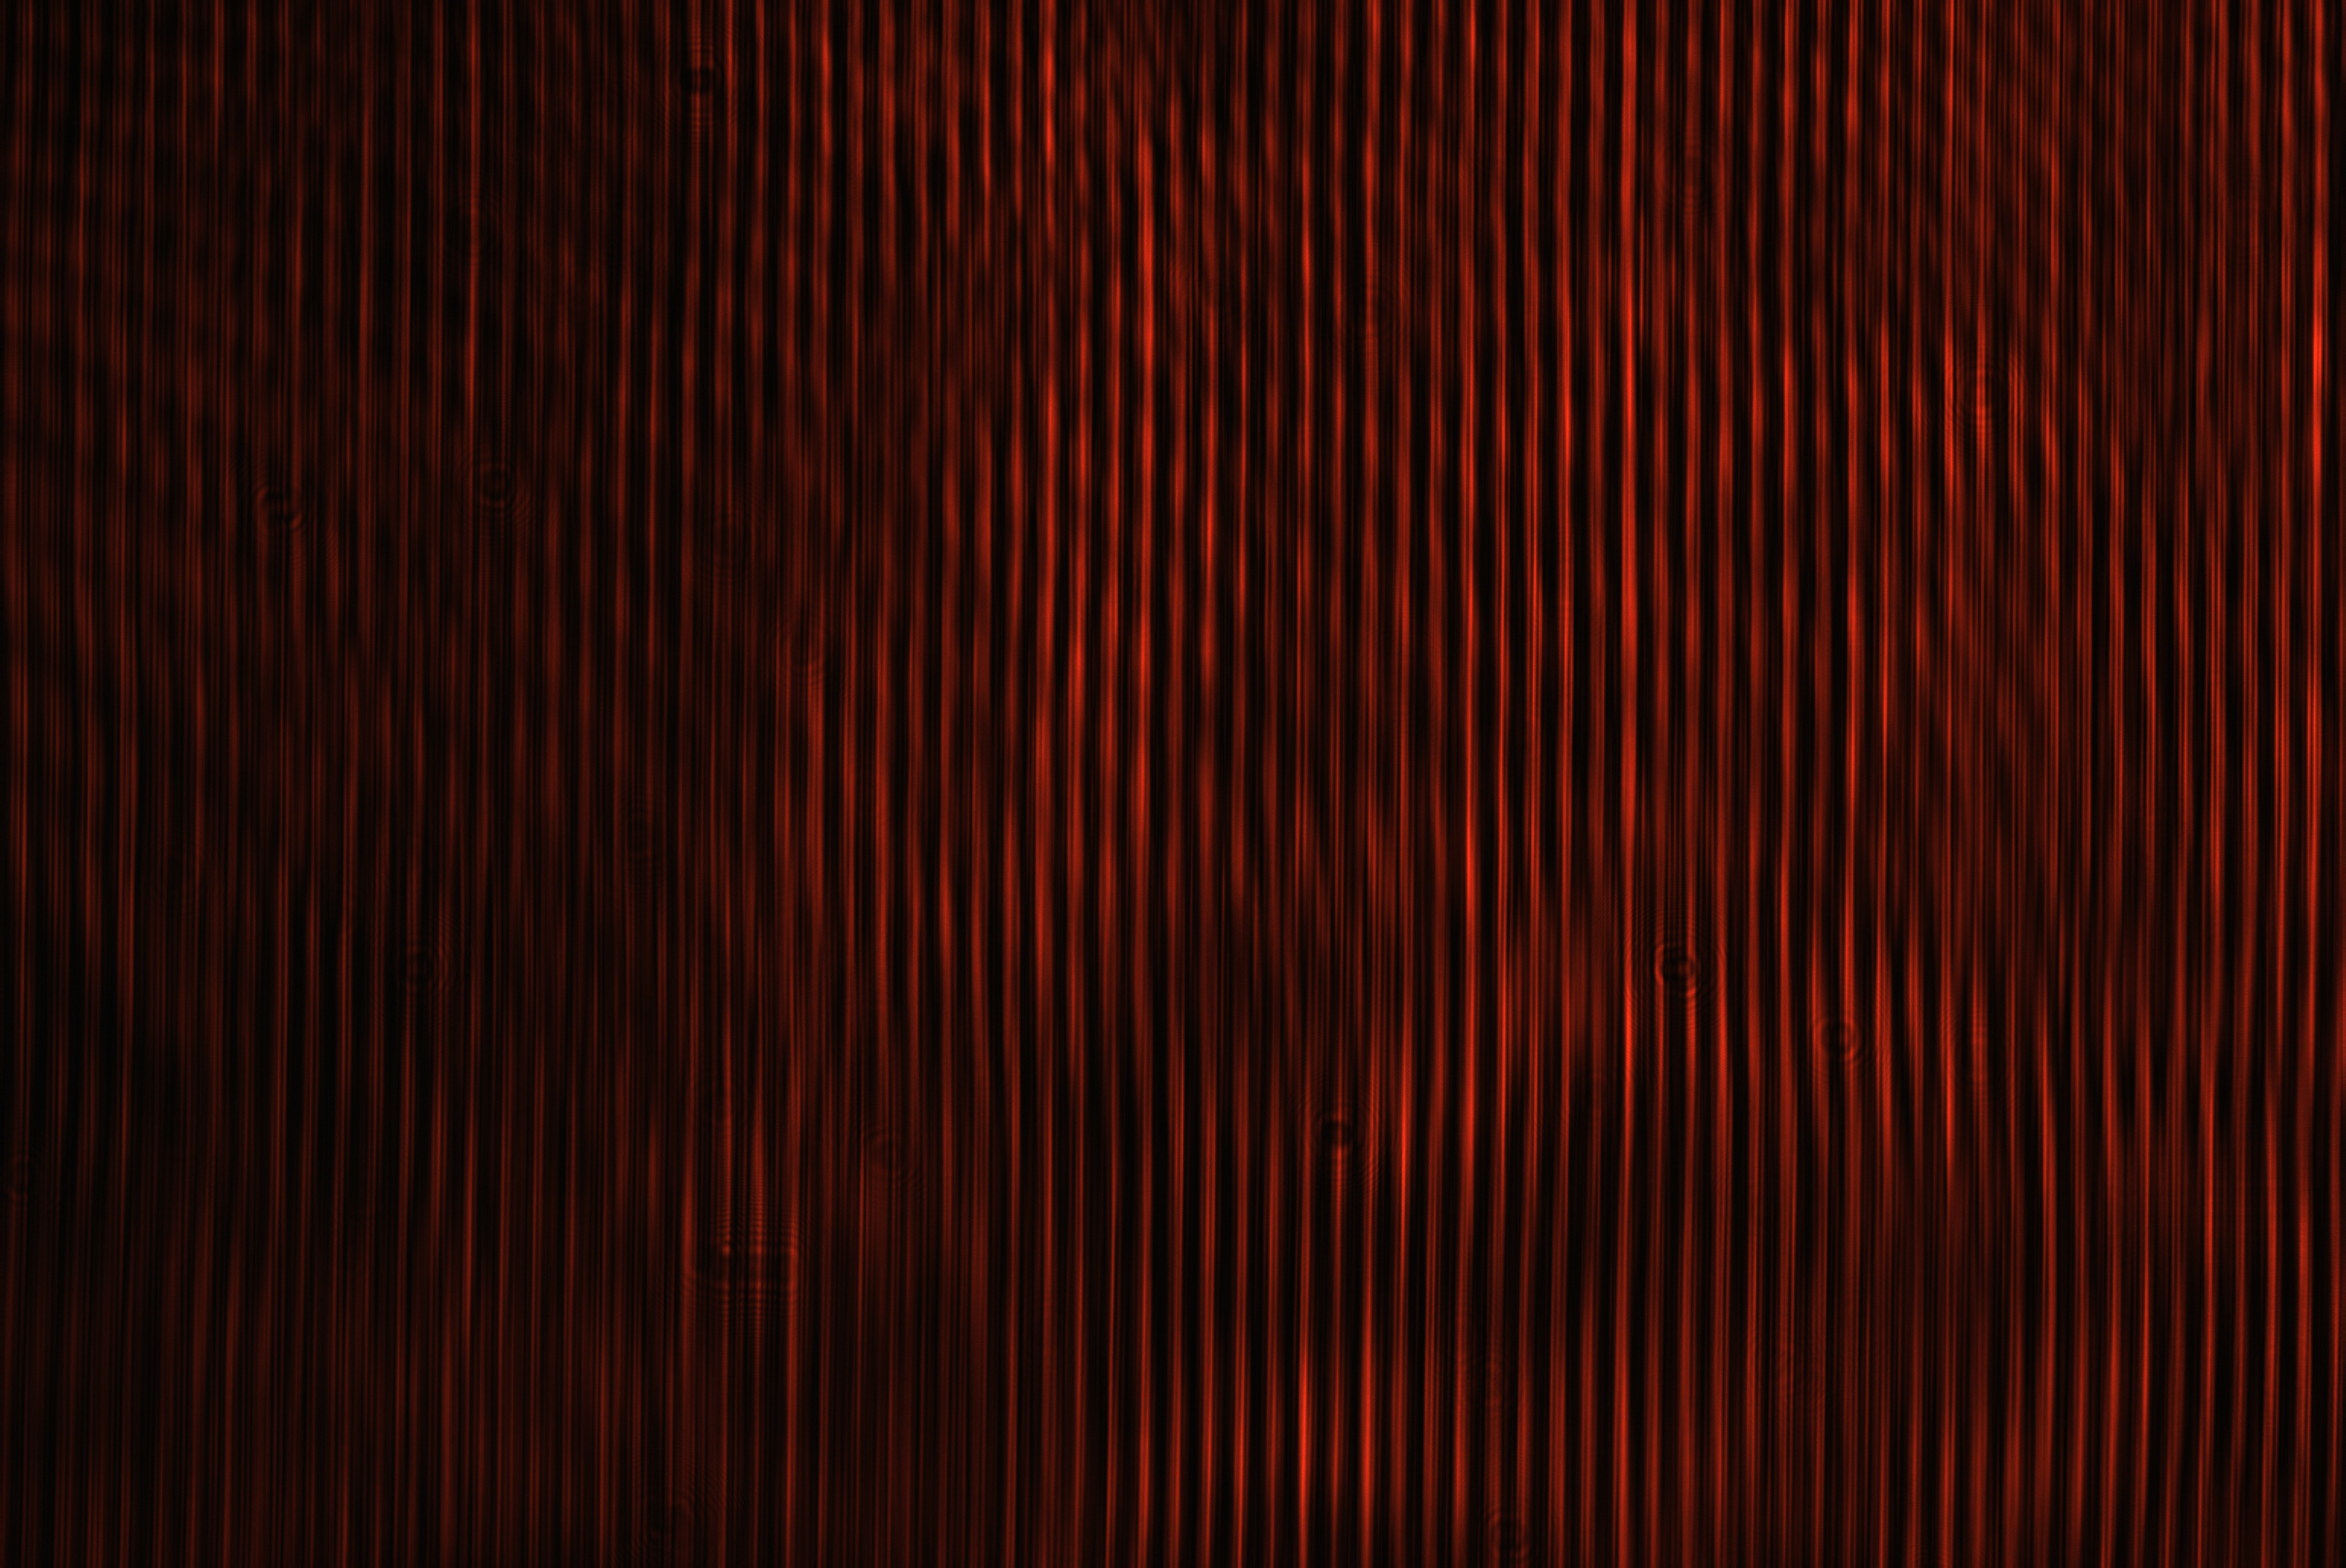
\includegraphics[width=0.3\textwidth]{C7.2/4/180.png}
	}%
	\subfloat[狭缝与水平夹$45^{\circ}$角]{
	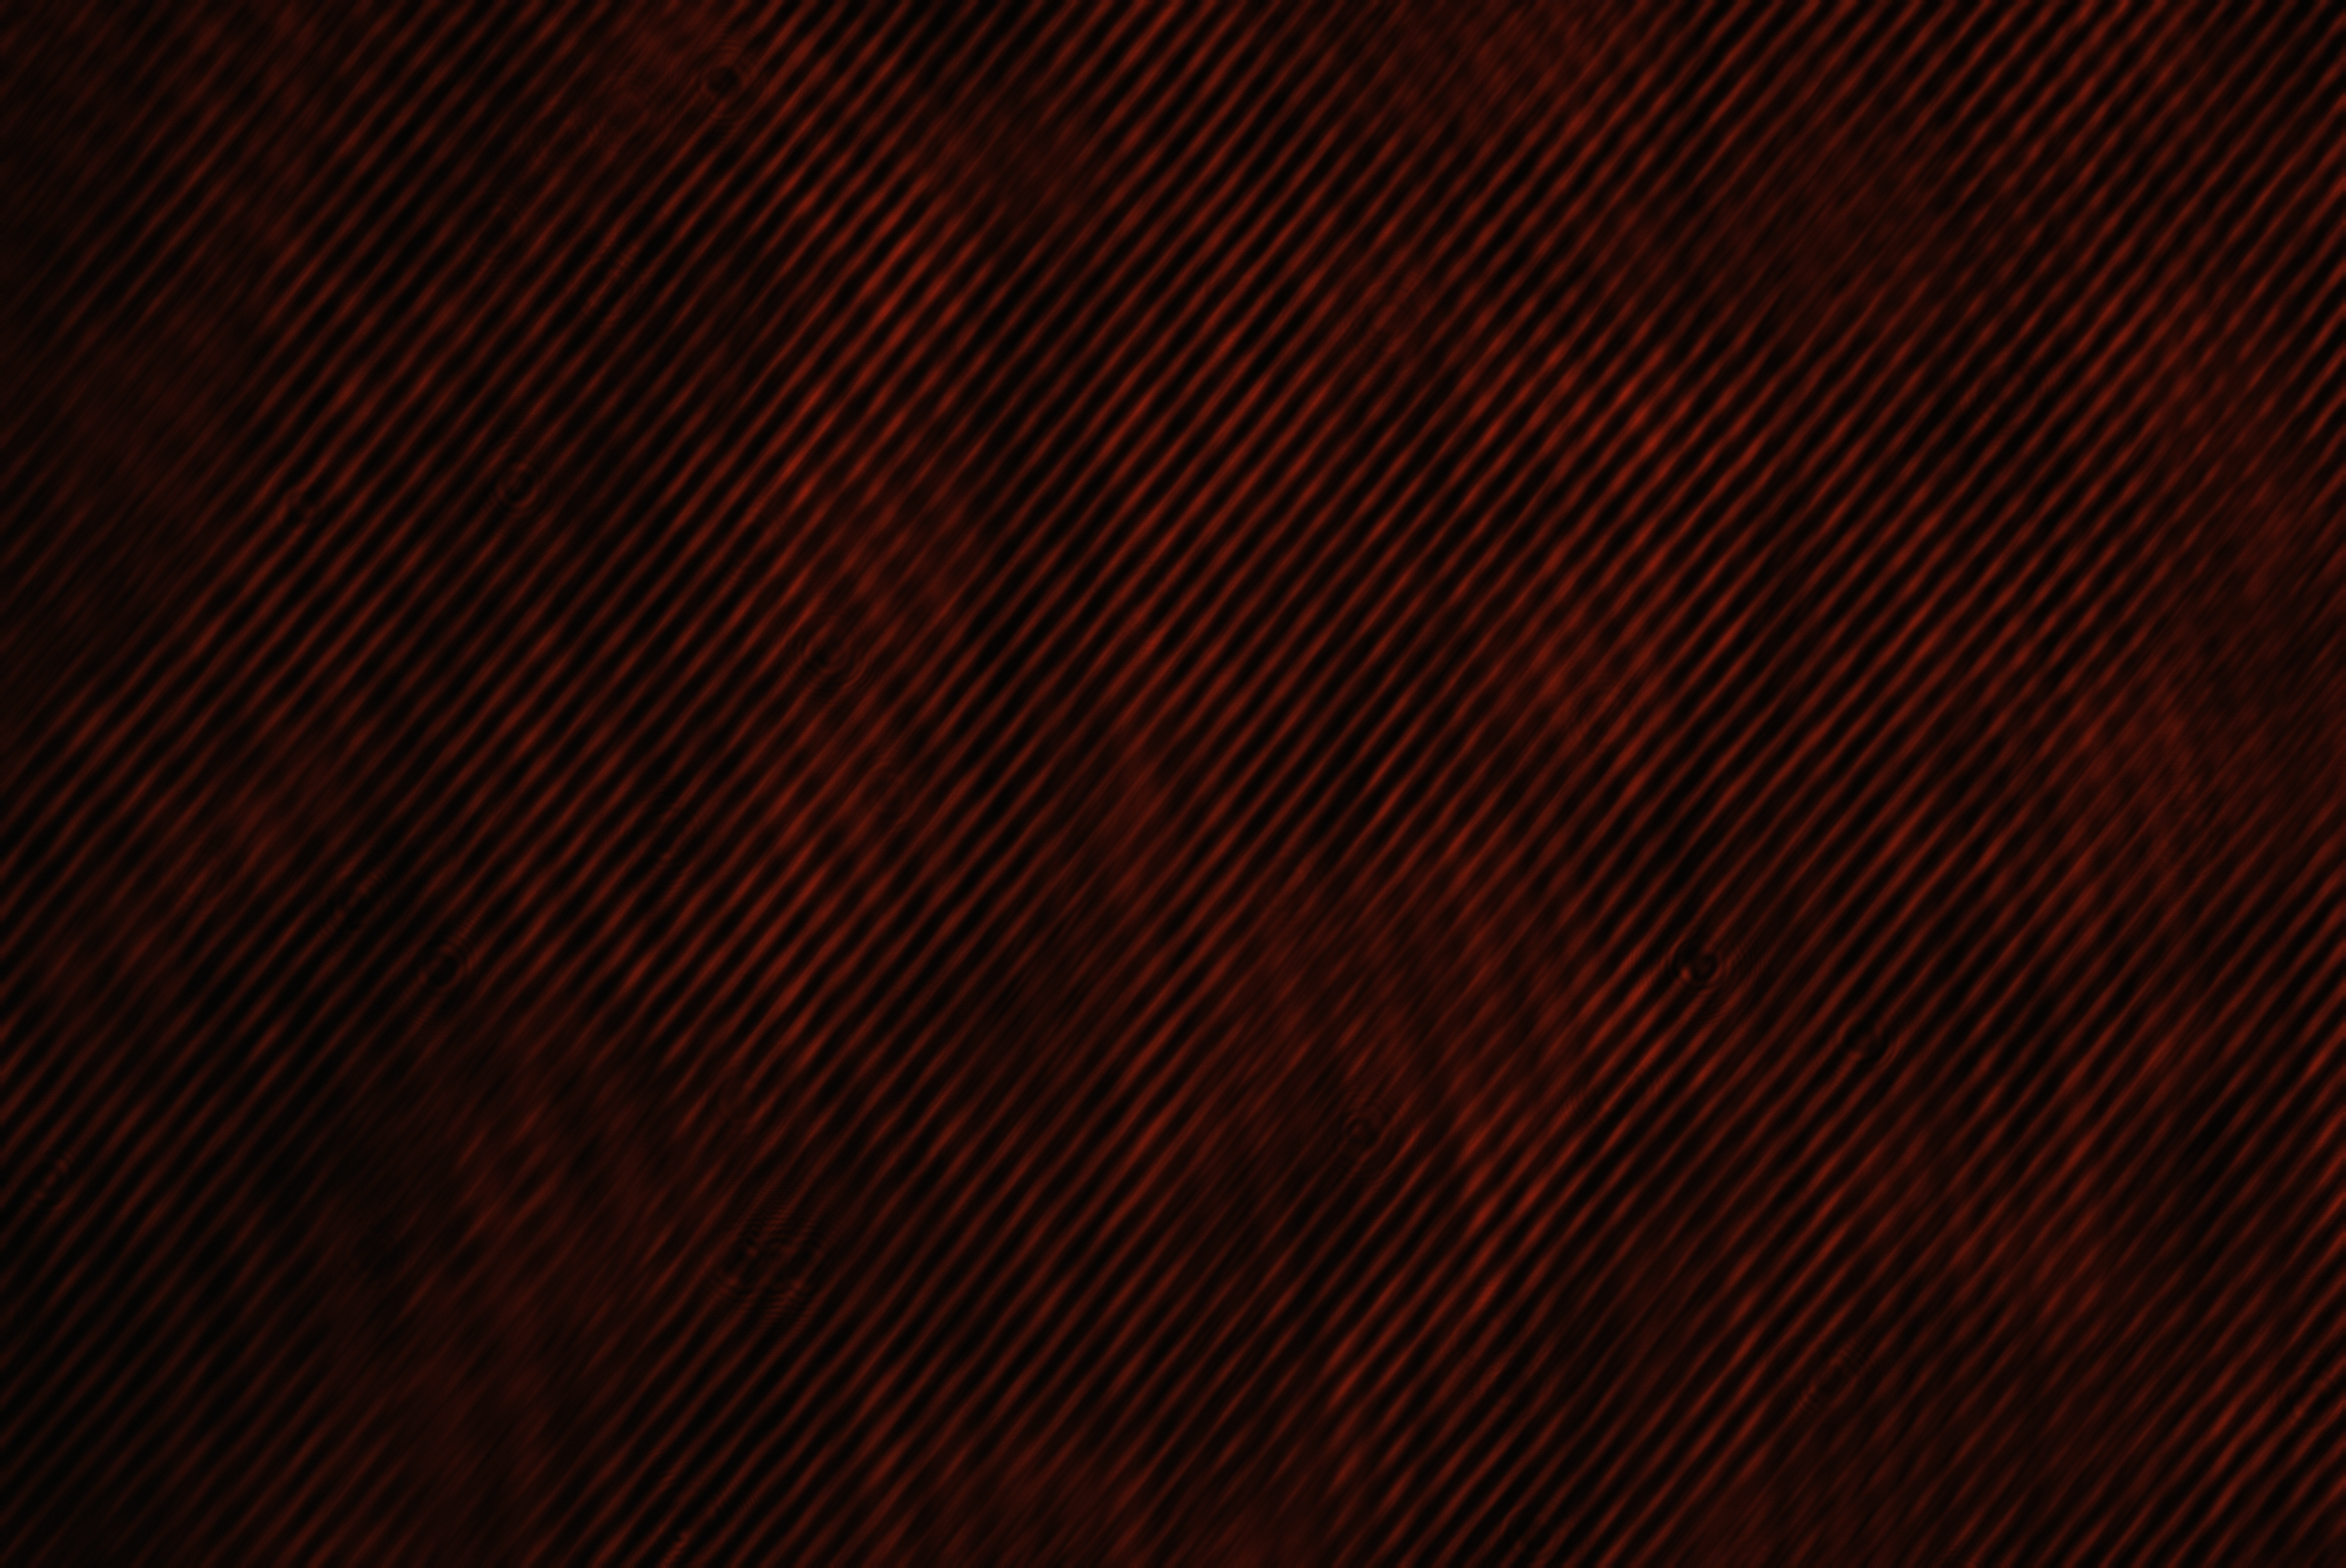
\includegraphics[width=0.3\textwidth]{C7.2/4/45.png}
	}%

	\subfloat[狭缝垂直]{
		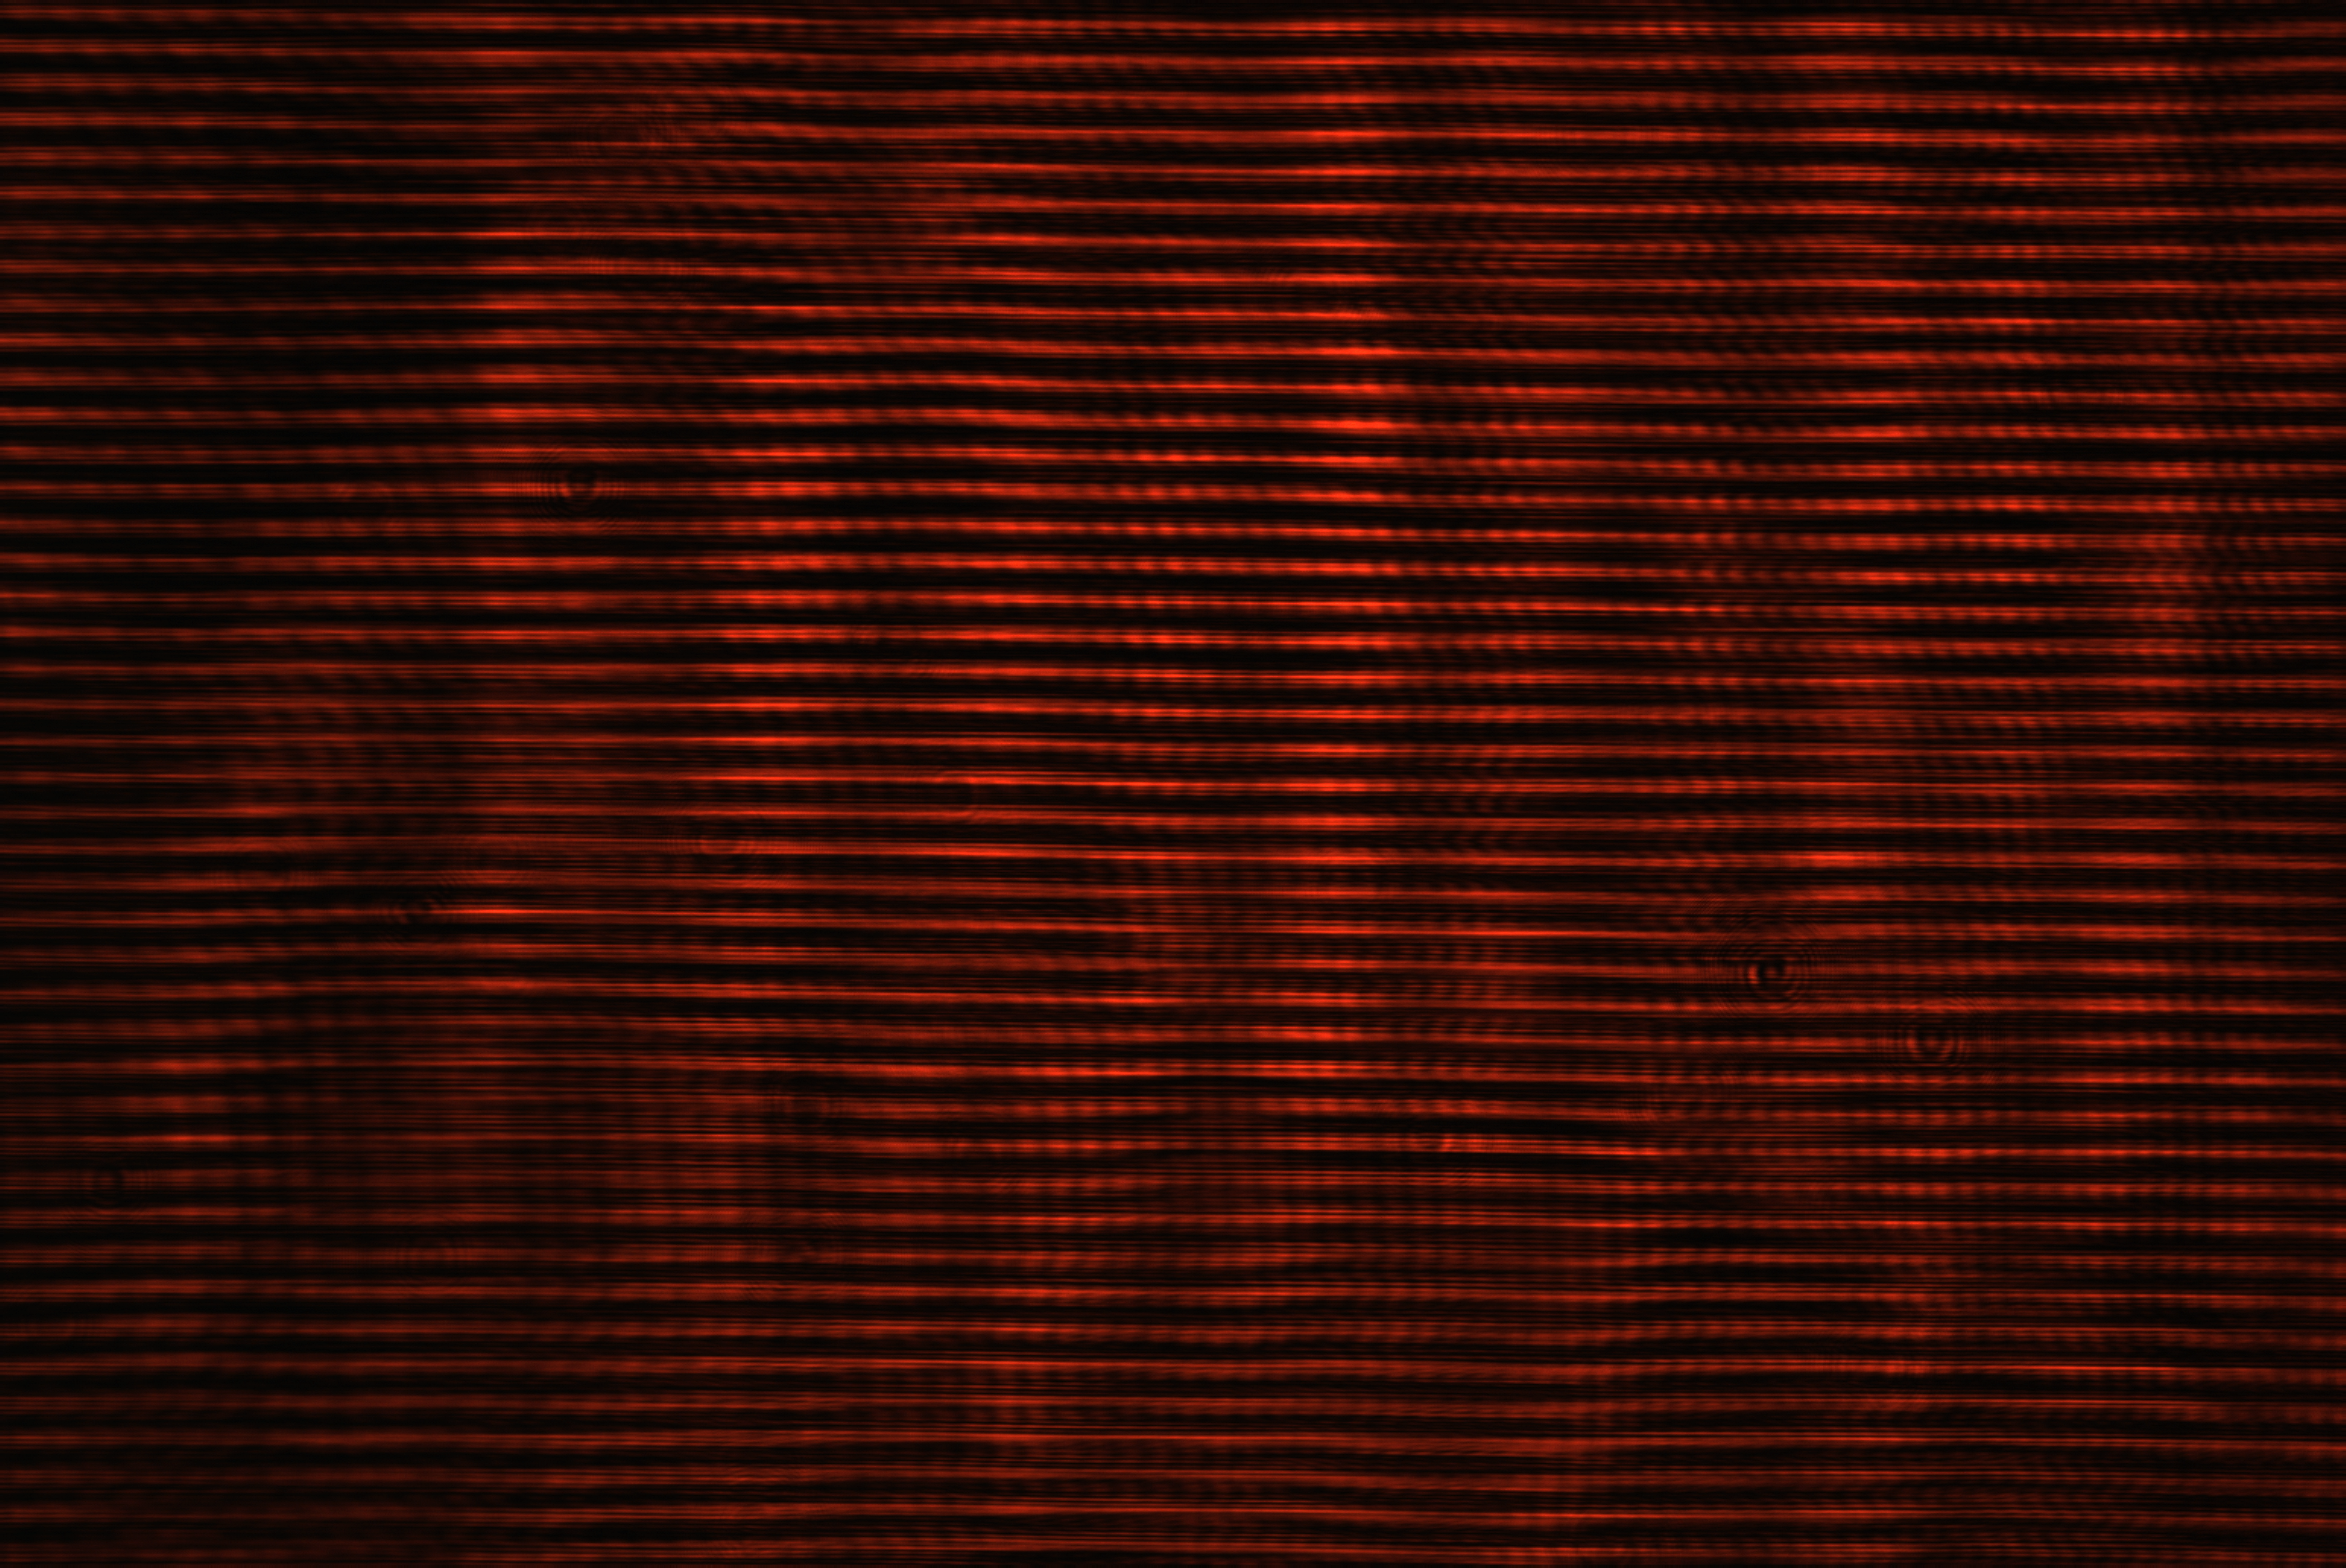
\includegraphics[width=0.3\textwidth]{C7.2/4/90.png}
	}%
	\subfloat[狭缝与水平夹$135^{\circ}$角]{
	
\includegraphics[width=0.3\textwidth]{C7.2/4/135.png}
	}%
	\caption{方向滤波成像}
	\label{fig:dir}
\end{figure}

分析实验结果可知,水平放置的狭缝得
到竖直条纹;竖直放置的狭缝得到水平条纹;
$45^{\circ}$放置的得到 $135^{\circ}$条纹;$135^{\circ}$放置的得
到$45^{\circ}$条纹。这是因为二维正交光栅的频谱
是一个二维的点阵,即包含了水平 x、竖直
y 方向上的频谱信息,而狭缝的放置方式不
同,导致部分信息丢失,只保留特定方向上
的频率信息,所以最终成像也只有该方向上
的振幅得以还原。

计算不同角度狭缝成像的条纹间距:
\begin{table}[H]
	\centering
	  \begin{tabular}{ccccc}
	  \toprule
	  狭缝倾斜角度&$0^{\circ}$ & $45^{\circ}$ &$90^{\circ}$ & $135^{\circ}$   \\
	  \midrule
	  十条条纹间距/pi & 446  & 325 &489& 338 \\
	  \bottomrule
	  \end{tabular}
	\caption{不同角度狭缝成像的条纹间距}
	\label{tab:distance}
\end{table}

\begin{equation*}
	\frac{426+479}{345+348}\approx 1.41\approx \sqrt{2}
\end{equation*}

由夫琅和费衍射可知:
\begin{equation*}
	dsin\theta=k\lambda
\end{equation*}

其中,由于像面较远,故可以认为条纹间距正比$sin\theta$;二维点阵的对角线上的两光点间距为边两光点的$\sqrt{2}$倍,即
$d_s=\sqrt{2} d$
故当激光波长不变时,$sin\theta$变为$\frac{\sqrt{2}}{2}$倍。故水平、竖直方向的条纹是45˚、135˚方向上的条纹间距的$\sqrt{2}$倍。
  
\subsection{基于空间光调制器的全息实验}
\subsubsection{计算全息成像}
\begin{figure}[H]
	\centering
	\subfloat[原图]{
	\includegraphics[width=0.25\textwidth]{C7.3/1/SYSUlogo.png}
	}
	\subfloat[计算全息图]{
	\includegraphics[width=0.3\textwidth]{C7.3/1/HoloFFT_SYSUlogo_Amplitude.png}
	}

	\subfloat[效果图]{
		\includegraphics[width=0.3\textwidth]{C7.3/1/ReconstrFFT_SYSUlogo_Amplitude.png}
	}
	\subfloat[计算全息成像]{
		\includegraphics[width=0.3\textwidth]{C7.3/1/1.2.png}
	}
	\caption{计算全息成像}
	\label{fig:holo1}
\end{figure}

由图\ref{fig:holo1}显示的全息图原图发现图像中央的亮斑为衍射产生亮斑。
仔细观察图像,发现所呈图像产生了一定的畸变,且图像精细度较低。


\subsubsection{数字全息成像}
\begin{figure}[H]
	\centering
	\subfloat[参考光间干涉图像]{
	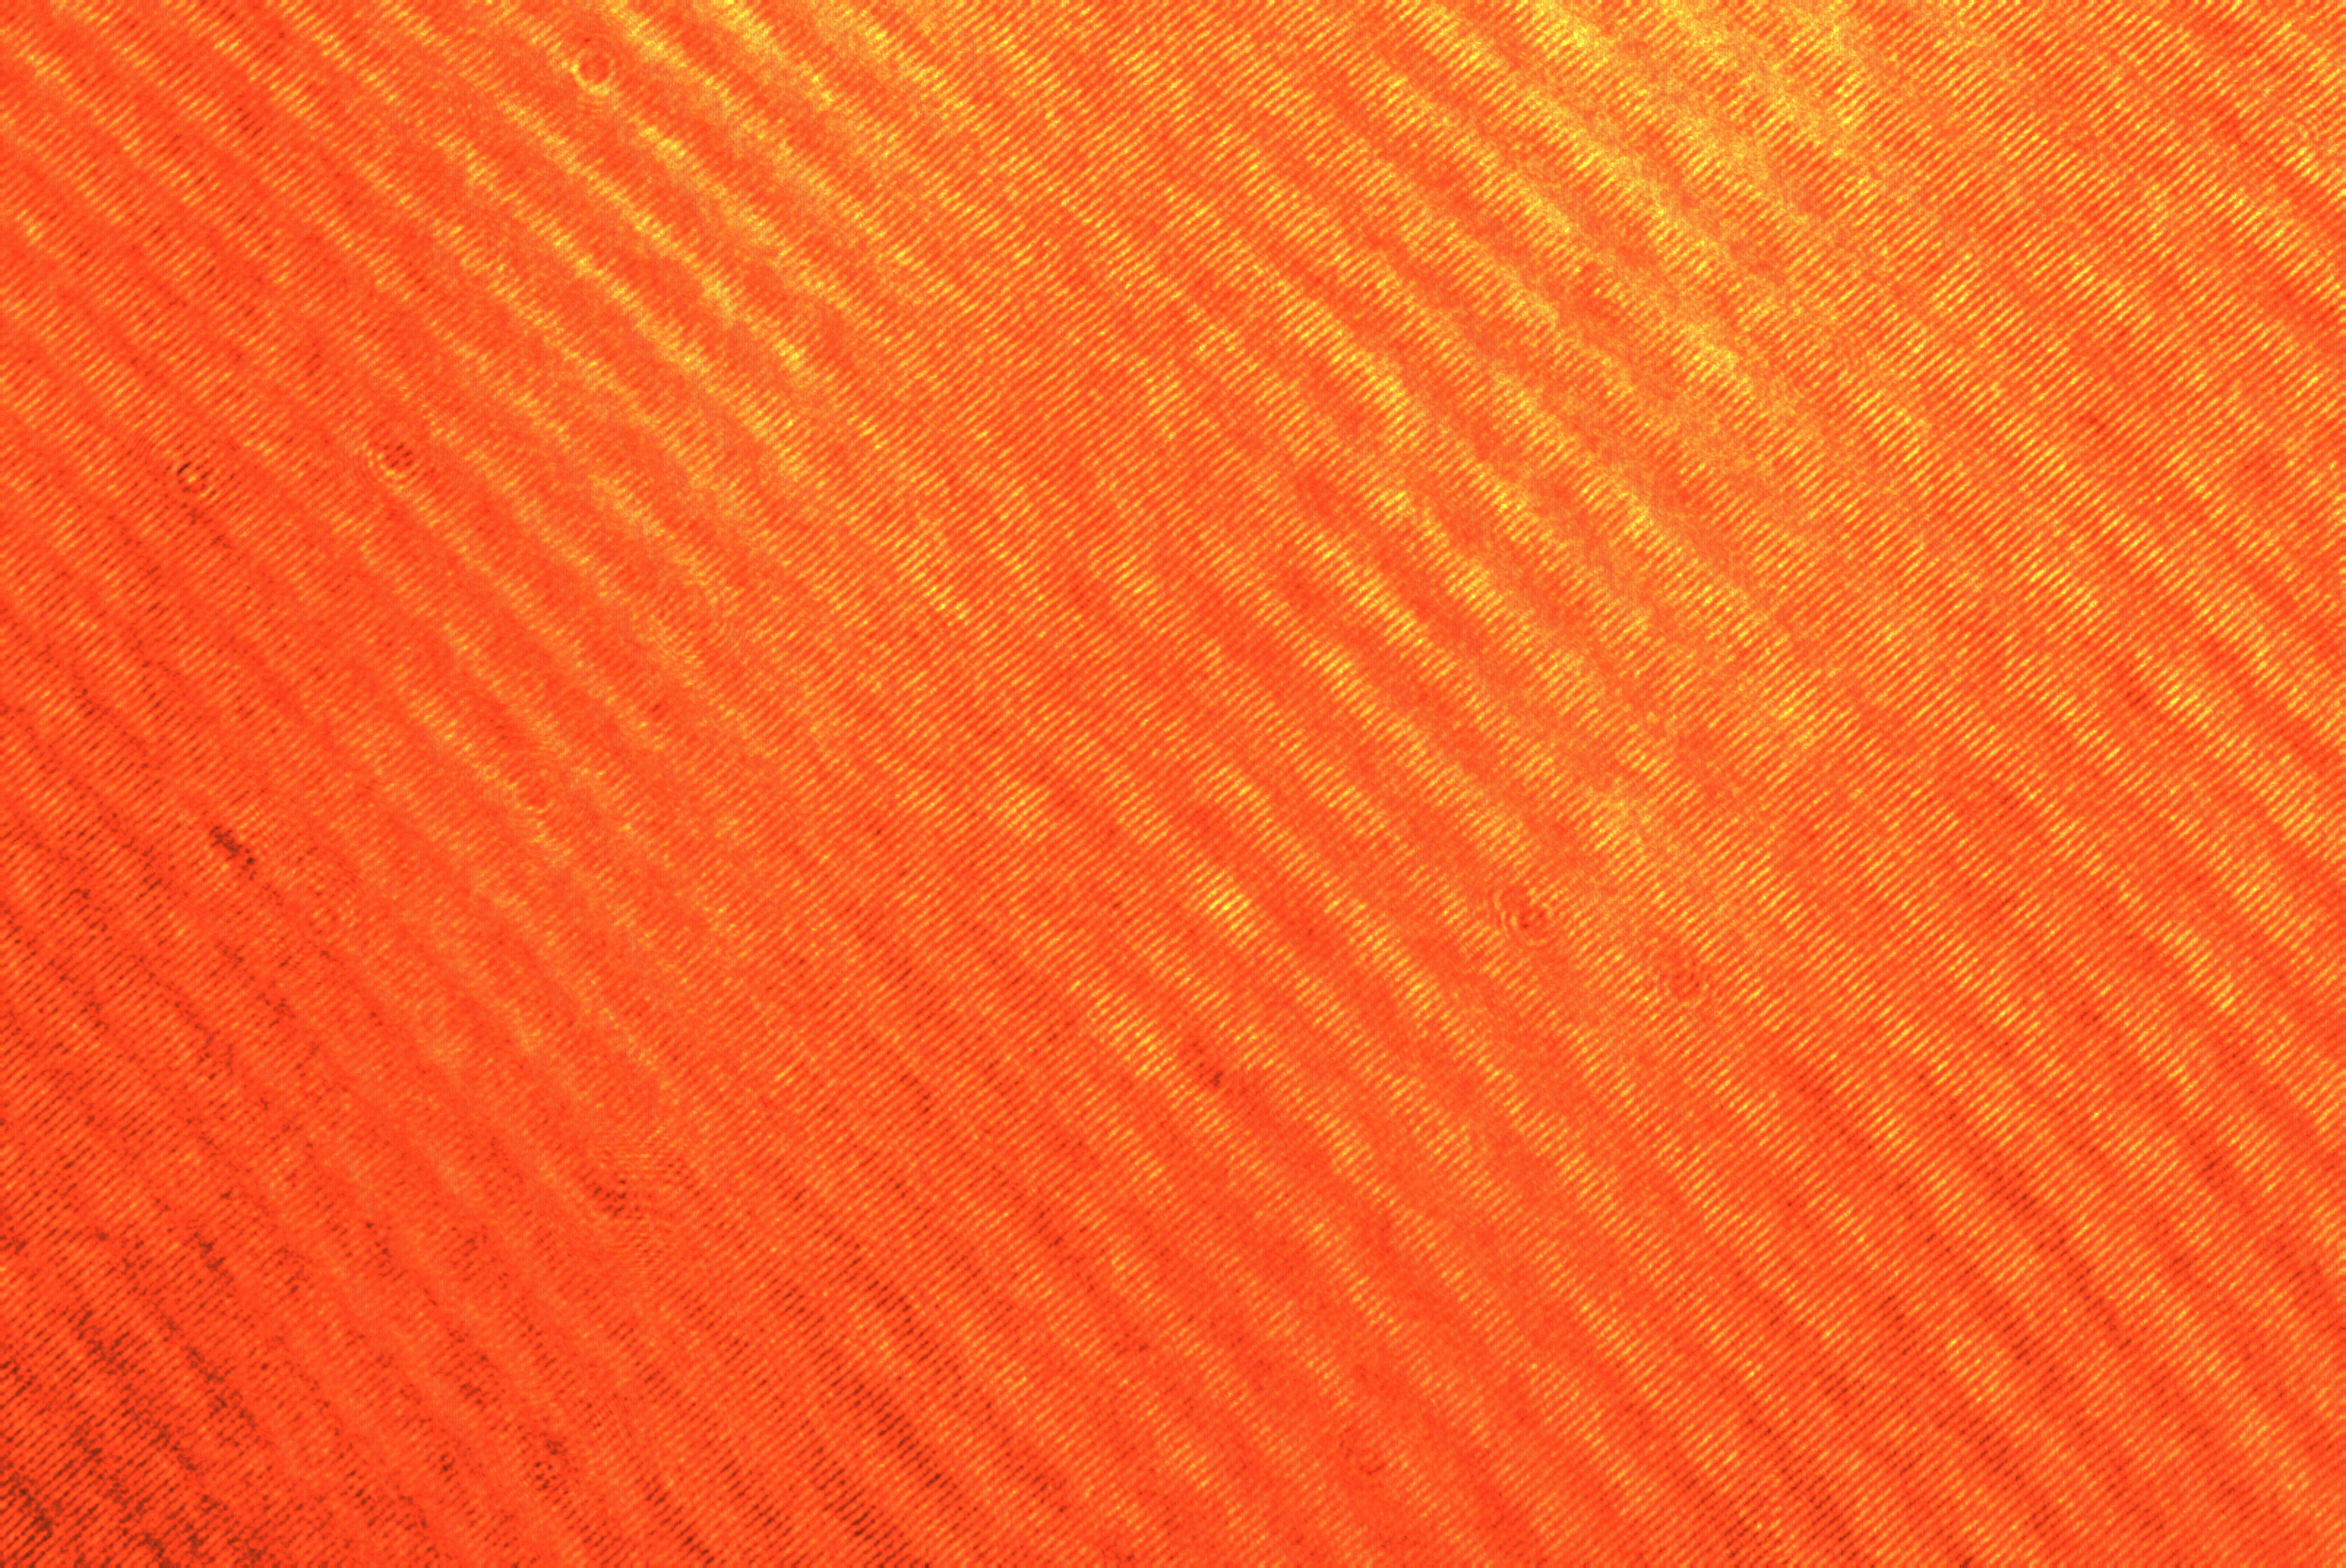
\includegraphics[width=0.3\textwidth]{C7.3/2/ref.png}
	}
	\subfloat[计算再现像]{
	\includegraphics[width=0.25\textwidth]{C7.3/2/Reconstruction_ref_Fresnel.png}
	}

	\subfloat[参考光与物光干涉图像]{
		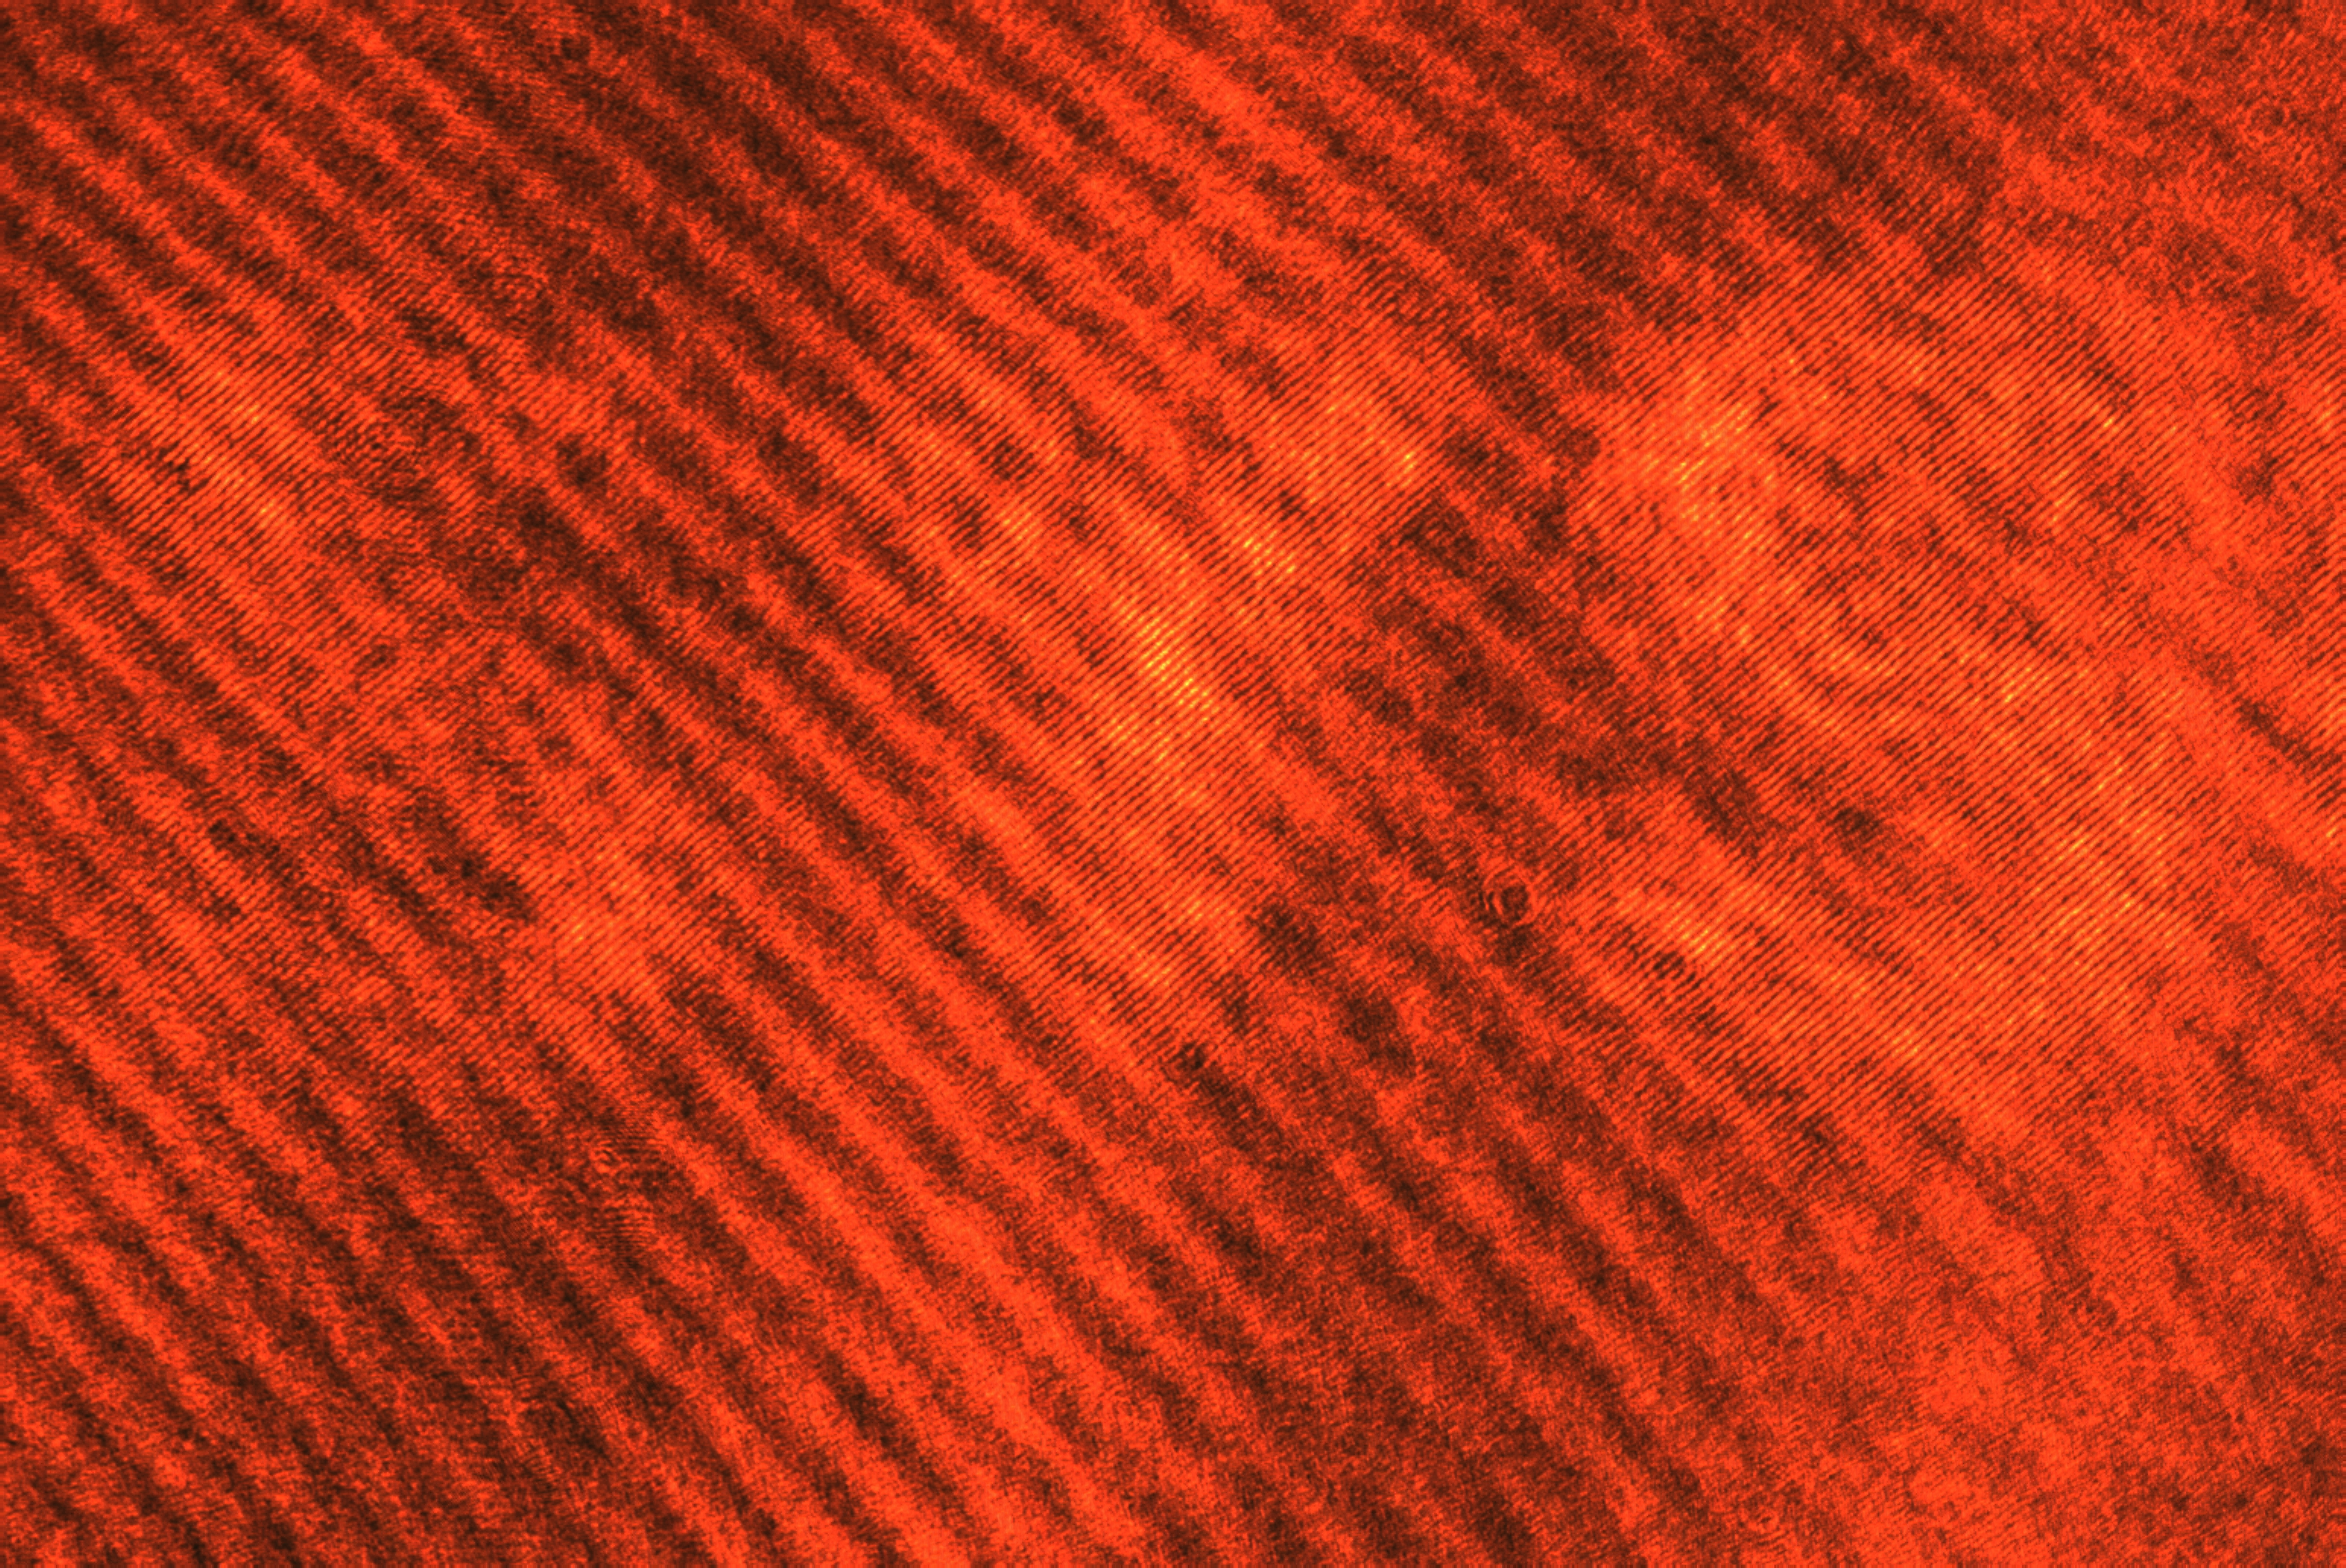
\includegraphics[width=0.3\textwidth]{C7.3/2/2.1.png}
	}
	\subfloat[计算再现像]{
		\includegraphics[width=0.25\textwidth]{C7.3/2/Reconstruction_2.1_Fresnel.png}
	}
	\caption{数字全息成像}
	\label{fig:holo2}
\end{figure}

由实验中的再现像可以看出,再现像存在明显的SYS字母,其周边存在较淡的SYS,为此像的衍射像。

\section{讨~~~论}
本次实验通过使用空间光调制器(SLM),测量其振幅调制特性,测量基于SLM产生的光学畸变。
利用多种光学仪器完成空间滤波、高通滤波、低通滤波、方向滤波以及完成数字全息与计算全息的实验。

测量空间光调制器的振幅调制曲线时灯光和计算机屏幕的亮度在灰度值较小时(0--100)对光功率计的读数有影响,造成实验误差,可以用幕布或纸板遮挡住计算机屏幕和灯光,或者调低计算机屏幕的亮度。
同时造成误差的有光功率计读数不稳定,一直处于波动状态,读数困难。在实验过程中,采取灰度的进步步长为10,若想使实验曲线更加精确,缩小步长或进行参数化扫描。

测量透镜畸变时调节光路十分重要,光路可能不完全等高同轴,导致图像很不对称,对实验结果造成一定影响。
实验中需因不同实验参数而调整光学元件间不同的距离,调整光学元件时距离上可能出现误差,导致缩小或放大的倍数不准,无法得到实际的畸变率。
在利用画图软件读取像素差时,一方面可能因为肉眼读数造成偏差,精度大致$\pm 5$左右,另一方面由于图像没有绝对的水平和竖直,使得读到的差值是其边在竖直(水平)方向的投影,造成一定误差。

滤波实验中在调节光学元件的距离时,由于手动测量的误差,导致实际距离与理论距离产生差异,导致CCD不严格位于傅立叶面上,导致误差的产生。

计算衍射场时,为使衍射场更加接近均匀振幅场,通常在计算时对记录物体随机添加相位使其高低频成分能均能充分扩散,导致重建结果中产生散斑噪声。
由于空间光调制器调制动态范围和精度有限,全息图的实际显示能力无法达到理论计算的效果。
在实际全息图的记录中,由于噪声、照明光场的不均匀性、物光衍射光场的调制和CCD动态范围的影响,难以记录到理想的数字全息图。除了存在理想全息图再现时的光场外,还可能存在若干低频和高频次频。在实际记录时,这些次谱混杂在物光信息中,难以滤除。


\section{结~~~论}
空间光调制器的振幅调制曲线整体呈 S 型,证明在偏振片正交的情况下,SLM 的透射率随写入信号的变化存
在阈值电压和饱和电压。当写入信号电压低于阈值电压,空间光调制器处于关态(暗态);当写入信号电压高于
饱和电压,透射光达到最大透过率,空间光调制器处于开态(亮态)。

使用CCD 拍摄不同焦距的透镜,不同缩小倍数棋盘格畸变的情况,棋盘格成像均发生枕形畸变。发现成像中距离中心位置越
近的点畸变越小,距离中心位置越远的点畸变越大。同一焦距同一放大倍数所
对应的相同距离不同方向的四个点的畸变值有差异,水平方向与竖直方向的畸变值不同,这说明对于每个透镜
组成的光学系统而言,并不是完全球对称,实验光路存在一定偏差。

对比通过低通滤波的像和原像,最明显的区别是“光”字内部的网格被过滤了,
保留下来的网格的低频信息是一个基本均匀的光照,所以最终
的图像是消去了网纹的光字。而通过高通滤波器的像与原像相比,区别在于前者更容易观察细节,锐化度更高。
这是因为高频代表的细节被保留,低频对应的像被削弱,相同的低频成分被滤去,所以提高了对比度。

二维正交光栅的频谱是一个二维的点阵,即包含了水平 x、竖直 y
方向上的频谱信息。因为方向滤波狭缝的放置方式不同,导致部分信息丢失,只保留特定方向上的频率信息,所以最终成像
也只有该方向上的振幅得以还原。

全息图原图的图像中央的亮斑为衍射产生亮斑。仔细观察图像,发现所呈图像产生了一定的畸变,且图像精细度较低。
由实验中的再现像可以看出,再现像存在明显的 SYS 字母,其周边存在较淡的SYS,为此像的衍射像。


\newpage
\printbibliography[title=参考文献] 
\clearpage

	 
\section*{\LARGE 附录A}
\section*{【思考题】}
\subsection*{1. 本实验所用的空间光调制器是哪种类型的空间光调制器?}
透射式电寻址空间光调制器。
\subsection*{2. 为什么同一缩小、放大倍数的棋盘格,缩小的棋盘格的畸变要比放大的棋盘格的畸变大?}
因为畸变的大小与该点与光轴距离
大小成正比。放大像时,视野内任一一点距
离光轴的距离都小于缩小像时视野内同一
点的距离,故而视野内同一点,在放大像中
的畸变会小于在缩小像里的畸变。
\subsection*{3. 运用阿贝成像原理,说明实物一维光栅与空间光调制器输入的一维光栅的频谱差异原因,
综合解释“验证阿贝成像原理(一)”和“验证阿贝成像原理(二)”所看到的现象。}
由于SLM 中不透明电极会阻挡一部分读出光,故SLM 液晶面板就像一个网格,
会将加载的一幅连续的图案进行分割,即空间数字化。
除了加载的图案会发生衍射外,网格结构也会使读出光发生衍射。
一维光栅网格化后的图案可以看作是一个正交的二维光栅,因此用SLM 作为光阑进行衍射实验时,
其空间频谱相对于实物光栅,在竖直方向上会有频谱信息存在,表现为二维的频谱图案。验证阿贝成像原理(一)
和验证阿贝成像原理(二)在实验现象上的不同,一是表现在频谱样式的差别;
二是表现在CCD抓取的图片上,实物的像只有竖条纹,而SLM作为光阑的像除了竖条纹,
还有细微的横条纹可见,并且由于实际操作中SLM前后的两个偏振器并不是完全正交的,
导致图片的对比度没有实物光栅高;三是在狭缝很小但不为0时,实物光栅的像是非常模糊、暗的不规则光斑,
这是零频亮部分通过的结果,而SLM作为光栅的像会出现密集的横条纹,如前所述,这是网格化后的二维正交光栅图案横向结构的像。
其差异的本质在于,SLM作为光栅实际上是在普通一维光栅的透过处变成了二维正交光栅结构。
\subsection*{4. 如何从阿贝成像原理来理解显微镜(或望远镜)的分辨本领?为什么说一定孔径的显微镜只
能具有有限的分辨本领,不能用增大放大倍数的办法来无限制提高其分辨样品细节的能力?}
由阿贝成像原理可知,如果所有空间频率的光信息都能在像面汇聚,那么所成像与物是完全一样的。
然而实际上由于成像透镜孔径有限,总有一部分衍射角较大的高频信息不能进入透镜而丢失,
这就导致成像不能和实物完全一样,在细节上一定会有损失。而显微镜(望远镜)作为一个物镜成像系统,
无论其放大率有多高,由于物体进入透镜总会损失一部分代表细节的高频信息,所以其分辨率一定会受到限制。
以一维光栅作为物为例,如果光栅间距小至使$\pm 1$级光波都无法通过透镜,
那么在频谱面上只有0级谱点,经过二次成像后就只是光照均匀的光斑而没有光栅的图案,
无论怎样放大,都不能分辨出光栅的图案。

\subsection*{5. 分析影响计算全息成像效果的因素。}
计算方式、编码方式、再现方式、绘制和缩小方式。
\subsection*{6. 尝试编写计算全息及数字全息的代码。}
代码见附录C
\begin{figure}[H]
	\centering
	\subfloat[振幅型傅里叶全息图]{
	\includegraphics[width=0.4\textwidth]{fig/code1.png}
	}
	\subfloat[全息图再现像]{
		\includegraphics[width=0.4\textwidth]{fig/output.png}
	}
	\caption{}
\end{figure}

\newpage
\section*{\LARGE 附录B}
\section*{【表格】}

\begin{table*}[htbp]
	\centering
	\resizebox{\linewidth}{!}{
	  \begin{tabular}{llrrrrrrrrrrrrr}
	  Lab   & Checker & \multicolumn{1}{l}{f} & \multicolumn{1}{l}{beta} & \multicolumn{1}{l}{s1} & \multicolumn{1}{l}{s2} & \multicolumn{1}{l}{X$\_$g} & \multicolumn{1}{l}{Y$\_$g} & \multicolumn{1}{l}{XY$\_$g} & \multicolumn{1}{l}{Center$\_$x$\_$p} & \multicolumn{1}{l}{Center$\_$y$\_$p} & \multicolumn{1}{l}{X$\_$x$\_$p} & \multicolumn{1}{l}{Y$\_$y$\_$p} & \multicolumn{1}{l}{XY$\_$x$\_$p} & \multicolumn{1}{l}{XY$\_$y$\_$p} \\
	  150$\_$4 & A     & 150   & 0.25  & 750   & 187.5 & 2     & 2     & 1.5   & 984   & 706   & 1505  & 179   & 1374  & 324 \\
	  70$\_$4 & A     & 70    & 0.25  & 350   & 87.5  & 2     & 2     & 1.5   & 1089  & 752   & 1662  & 177   & 1520  & 321 \\
	  50$\_$4 & A     & 50    & 0.25  & 250   & 62.5  & 2     & 2     & 1.5   & 1085  & 767   & 1682  & 208   & 1532  & 337 \\
	  70$\_$2 & A     & 70    & 0.5   & 210   & 105   & 1     & 1     & 1     & 1054  & 830   & 1556  & 320   & 1562  & 304 \\
	  70$\_$6 & A     & 70    & 0.166 & 490   & 81.64 & 2     & 2     & 1.5   & 1061  & 690   & 1466  & 315   & 1367  & 391 \\
	  48x64$\_$2X & B     & 70    & 2     & 210   & 105   & 2     & 2     & 1.5   & 977   & 734   & 1541  & 171   & 1393  & 314 \\
	  48x64$\_$4X & B     & 70    & 4     & 350   & 87.5  & 1     & 1     & 1     & 1071  & 683   & 1459  & 301   & 1459  & 301 \\
	  \end{tabular}}
	\caption{Input}
	\label{tab:s1}
  \end{table*}


\begin{table*}[htbp]
	\centering
	  \begin{tabular}{lr}
	  Par   & \multicolumn{1}{l}{Val} \\
	  Checker$\_$x$\_$p & 1024 \\
	  Checker$\_$y$\_$p & 768 \\
	  Checker$\_$A$\_$x$\_$g & 8 \\
	  Checker$\_$A$\_$y$\_$g & 6 \\
	  Checker$\_$B$\_$x$\_$g & 64 \\
	  Checker$\_$B$\_$y$\_$g & 48 \\
	  SLM$\_$d & 26 \\
	  CCD$\_$d & 3.2 \\
	  \end{tabular}
	\caption{Parameter}
	\label{tab:s2}
  \end{table*}

\begin{table*}[htbp]
	\centering
	\resizebox{\linewidth}{!}{
	  \begin{tabular}{rrrrrrrrrrrr}
	  \multicolumn{1}{l}{X$\_$h1} & \multicolumn{1}{l}{Y$\_$h1} & \multicolumn{1}{l}{XY$\_$h1x} & \multicolumn{1}{l}{XY$\_$h1y} & \multicolumn{1}{l}{X$\_$h2} & \multicolumn{1}{l}{Y$\_$h2} & \multicolumn{1}{l}{XY$\_$h2x} & \multicolumn{1}{l}{XY$\_$h2y} & \multicolumn{1}{l}{X$\_$dh} & \multicolumn{1}{l}{Y$\_$dh} & \multicolumn{1}{l}{XY$\_$dhx} & \multicolumn{1}{l}{XY$\_$dhy} \\
	  1664  & 1664  & 1248  & 1248  & 1667.2 & 1686.4 & 1248  & 1222.4 & 3.2   & 22.4  & 0     & -25.6 \\
	  1664  & 1664  & 1248  & 1248  & 1833.6 & 1840  & 1379.2 & 1379.2 & 169.6 & 176   & 131.2 & 131.2 \\
	  1664  & 1664  & 1248  & 1248  & 1910.4 & 1788.8 & 1430.4 & 1376  & 246.4 & 124.8 & 182.4 & 128 \\
	  1664  & 1664  & 1664  & 1664  & 1606.4 & 1632  & 1625.6 & 1683.2 & -57.6 & -32   & -38.4 & 19.2 \\
	  1104.896 & 1104.896 & 828.672 & 828.672 & 1296  & 1200  & 979.2 & 956.8 & 191.104 & 95.104 & 150.528 & 128.128 \\
	  1664  & 1664  & 1248  & 1248  & 1804.8 & 1801.6 & 1331.2 & 1344  & 140.8 & 137.6 & 83.2  & 96 \\
	  1664  & 1664  & 1664  & 1664  & 1241.6 & 1222.4 & 1241.6 & 1222.4 & -422.4 & -441.6 & -422.4 & -441.6 \\
	  \end{tabular}}
	\caption{Output}
	\label{tab:s3}
  \end{table*}
  
  

\newpage
\section*{\LARGE 附录C}
\section*{【代码】}
源代码位于:\url{https://github.com/MoRunbing/Physics_Experiment_Report/blob/main/C7}

作图
\begin{lstlisting}	
library(ggplot2)

power<-c(0.063,0.075,0.078,0.080,0.095,
		0.112,0.137,0.151,0.235,0.444,
		0.568,0.736,1.43,2.18,3.59,
		4.75,6.92,10.02,13.51,16.74,
		19.58,20.81,21.64,21.75,21.83,21.91)
data<-data.frame(gray=seq(0,250,by=10),power)

plot<-ggplot()+
  geom_line(data = data,aes(x = gray,y = power, colour="red"),size=1)+
  scale_y_continuous(breaks=seq(0, 23, 1)) +
  scale_x_continuous(breaks=seq(0, 260, 20))+
  labs(title="", x="灰度", y="光功率/um")+
  theme_classic()+ theme(legend.position = 'none')+
  theme(plot.title = element_text(hjust = 0.5))
ggsave("plot.png",plot)
\end{lstlisting}

% 识图
% \begin{lstlisting}
% 	import cv2
% 	import os

% 	file_pathname="D:\LaTeX\physics experiment\C7\C7.1"
% def read_path(file_pathname):
%     for filename in os.listdir(file_pathname):
%         print(filename)
%         image = cv2.imread(file_pathname+'/'+filename)

%         gray = cv2.cvtColor(image,cv2.COLOR_BGR2GRAY)
%         # cv2.imshow('1',gray)
%         bilateral = cv2.bilateralFilter(gray,15,75,75)
%         thresh = cv2.GaussianBlur(bilateral,(3,3),0)

%         for i in range(5):
%             thresh = cv2.GaussianBlur(thresh,(3,3),0)
%             dilated = cv2.dilate(thresh, (1, 1), iterations=1)

%         ret, thresh = cv2.threshold(dilated, 50, 255, cv2.THRESH_BINARY) 
%         thresh = cv2.GaussianBlur(thresh,(3,3),0)
%         canny = cv2.Canny(thresh, 10, 200, 3)

%         cnts = cv2.findContours(canny, cv2.RETR_EXTERNAL, cv2.CHAIN_APPROX_SIMPLE)
%         cnts = cnts[0] if len(cnts) == 2 else cnts[1]

%         minimum_area = 10000

%         for c in cnts:
%             area = cv2.contourArea(c)
%             if area > minimum_area:
%                 draw = cv2.drawContours(image, [c], -1, (0,255,0), 2)
%                 print(area)
                
%         cv2.imwrite("D:\LaTeX\physics experiment\C7\Fig"+"/"+filename[:-4:1]+" ref"+".png",draw) 
% read_path("D:\LaTeX\physics experiment\C7\C7.1")
% \end{lstlisting}

数据处理
\begin{lstlisting}
import numpy as np 
import pandas as pd
import matplotlib.pyplot as plt
import seaborn as sns
import sympy as sp

df_par = pd.read_csv('Input/Par.csv')
par = dict(zip(df_par["Par"], df_par["Val"]))
par["A_hx_pergrid"] = par["Checker_x_p"]*par["SLM_d"]/par["Checker_A_x_g"] # x-orientation Side length per grid of Checker A
par["A_hy_pergrid"] = par["Checker_y_p"]*par["SLM_d"]/par["Checker_A_y_g"] # y-orientation Side length per grid of Checker A

par["B_hx_pergrid"] = par["Checker_x_p"]*par["SLM_d"]/par["Checker_B_x_g"] # x-orientation Side length per grid of Checker B
par["B_hy_pergrid"] = par["Checker_y_p"]*par["SLM_d"]/par["Checker_B_y_g"] # y-orientation Side length per grid of Checker B
par

df2 = pd.read_csv('Input/Distortion.csv')

# ideal image height 
df2["X_h1"] = df2.apply(lambda x: x.X_g*par["A_hx_pergrid"]*x.beta if x.Checker == "A" else x.X_g*par["B_hx_pergrid"]*x.beta, axis=1) # X-orientation ideal image height 
df2["Y_h1"] = df2.apply(lambda x: x.Y_g*par["A_hy_pergrid"]*x.beta if x.Checker == "A" else x.Y_g*par["B_hy_pergrid"]*x.beta, axis=1) # Y-orientation ideal image height

df2["XY_h1x"] = df2.apply(lambda x: x.XY_g*par["A_hx_pergrid"]*x.beta if x.Checker == "A" else x.XY_g*par["B_hx_pergrid"]*x.beta, axis=1) # X-orientation ideal image height 
df2["XY_h1y"] = df2.apply(lambda x: x.XY_g*par["A_hy_pergrid"]*x.beta if x.Checker == "A" else x.XY_g*par["B_hy_pergrid"]*x.beta, axis=1) # Y-orientation ideal image height

# actual image height
df2["X_h2"] = (df2["X_x_p"]-df2["Center_x_p"])*par["CCD_d"] # X-orientation actual image height 
df2["Y_h2"] = -(df2["Y_y_p"]-df2["Center_y_p"])*par["CCD_d"] # Y-orientation actual image height

df2["XY_h2x"] = (df2["XY_x_p"]-df2["Center_x_p"])*par["CCD_d"] # XY-orientation actual image height (x comp.)
df2["XY_h2y"] = -(df2["XY_y_p"]-df2["Center_y_p"])*par["CCD_d"] # XY-orientation actual image height (y comp.)

# Diff
df2["X_dh"] = df2["X_h2"].abs() - df2["X_h1"].abs() # X-orientation Diff 
df2["Y_dh"] = df2["Y_h2"].abs() - df2["Y_h1"].abs() # Y-orientation Diff

df2["XY_dhx"] = df2["XY_h2x"].abs() - df2["XY_h1x"].abs() # XY-orientation Diff (x comp.)
df2["XY_dhy"] = df2["XY_h2y"].abs() - df2["XY_h1y"].abs() # XY-orientation Diff (y comp.)

# Distortion q
df2["X_q"] = (df2["X_dh"]/df2["X_h1"]).map(lambda x:format(x, '.2%')) # X-orientation Distortion q
df2["Y_q"] = (df2["Y_dh"]/df2["Y_h1"]).map(lambda x:format(x, '.2%')) # Y-orientation Distortion q

df2["XY_qx"] = (df2["XY_dhx"]/df2["XY_h1x"]).map(lambda x:format(x, '.2%')) # XY-orientation Distortion q (x comp.)
df2["XY_qy"] = (df2["XY_dhy"]/df2["XY_h1y"]).map(lambda x:format(x, '.2%')) # XY-orientation Distortion q (y comp.)
df2[["Lab", "X_dh", "Y_dh", "XY_dhx", "XY_dhy", "X_q", "Y_q", "XY_qx", "XY_qy"]]

df2.to_csv('Output/Distortion.csv', index=False)
\end{lstlisting}

全息图

\url{https://github.com/OptoManishK/Digital_Holography}

\end{document}
